\documentclass[12pt,a4paper,notitlepage,english]{article}
\usepackage[utf8]{inputenc}
\usepackage[title,titletoc,toc]{appendix}
\usepackage{amsmath}
\usepackage{amsfonts}
\usepackage{longtable}
\usepackage{amssymb}
\usepackage{pdflscape}
\usepackage{hyperref}
\usepackage{graphicx}
\usepackage[a4paper, left=.6in,right=.6in,top=.8in,bottom=.8in,]{geometry}
\usepackage{tabularx,ragged2e,booktabs,caption}
\usepackage{setspace}
\usepackage[dvipsnames]{xcolor}
\usepackage[colorinlistoftodos,textsize=tiny]{todonotes}
\setstretch{1.5}
\usepackage{tabularx, booktabs}
\usepackage{dcolumn} 
  \newcolumntype{d}[1]{D{.}{.}{#1}}    
\newcolumntype{Y}{>{\centering\arraybackslash}X}
\usepackage[T1]{fontenc}
\usepackage{babel}
\usepackage{epigraph}
\usepackage{url}
\usepackage[round,sort]{natbib}
\newcommand{\source}[1]{\caption*{\footnotesize Source: {#1}} }
\usepackage{float}
\usepackage[section]{placeins}
\usepackage{ctable}
\newcolumntype{?}{!{\vrule width 2pt}}
 \newcolumntype{d}[1]{D{.}{.}{#1}} 
\DeclareUnicodeCharacter{202F}{ }
\usepackage{comment}
\usepackage{tikz}
 

\author{
  Guillaume Daudin\thanks{Université Paris-Dauphine, PSL Research University, CNRS, 8007, IRD, 260, LEDa, DIAL, 75016, Paris, France. Sciences Po, OFCE, 75007, Paris. Corresponding author. E-mail: guillaume.daudin@dauphine.psl.eu}
  \and
  Elisa Maria Tirindelli\thanks{Trinity College Dublin, email: tirindee@tcd.ie}
}
\title{Not “easy to win”: \\ The British war on French trade, 1716-1822\thanks{The authors want to thanks Henning Hillmann and Philip Hoffman for sharing data with them. They also thanks Cyril Canet, Roger Knight, David Plouviez, Peter Solar and particpants at the IHS (London), Trinity College (Dublin) seminar in London, and at the AFSE, EHES, EHS, Réseau de Recherche pour l’innovation ad Toflit conferences}}
\date{}


\begin{document}

\maketitle


\begin{abstract}
International trade is one of the main issues at stake in the rivalry between powers. The
British war on French trade from the War of Austrian Succession to the fall of Napoleon gives
us a lesson on how to win it when outright destruction is not an option. We suggest a measure
of the achievements of a war on French trade. We present the policies implemented by Britain
to wage it: establishment of naval supremacy, overseas territorial capture, predation on French
ships and extension of this predation to neutral carriers. We show that long term success implied
a durable change in the structure of French trade. Finally, we compute that, compared to loses
inflicted on the French economy, waging this war on trade was a costly endeavor.
\end{abstract}


\section{Introduction} \label{introduction}

\epigraph{Savez-vous Messieurs ce qu’est une bataille navale ? On se rencontre, on se salue, on se canonne et la mer n’en reste pas moins salée.}{Maurepas, Navy Minister of Louis  \textsc{xv}, 1718-1748}

\maketitle

%Citer ?  Small and medium powers in global history: trade, conflicts and neutrality from the 18th to the 20th Centuries : edited by Jari Eloranta, Eric Golson, Peter Hedberg and Maria Cristina Moriera, London and New York, Routledge, 2019, 240 pp., &#8364;133.10 (hardback), ISBN 978-1-138-74454-7
%
\todo[inline, color = YellowOrange]{1) The link between war and trade is an important question, as long-term crippling of enemy's international trade is a strategic war aim. \\
2) There is some debate on whether war is a good way to reduce the long-term international trade of a country. There is little study on the mechanism through which wars affect trade effectively \\
3) By studying one of the most important war on trade ever conducted, this paper shows that reducing trade is difficult, requires the use of multiple war measures and works through imposing structural changes on the enemy's trade structure, not simply by reducing its trade.}
\todo[inline, color =YellowOrange ]{And so, outline... 1. What policies were implemented? 2. Impacting trade through war is difficult (loss function and cost/benefit analysis) 3. It works through imposing long-term structural change. 4. What policies are good for that? }
\todo[inline, color = YellowOrange]{That looks similar to what you are suggesting?}
\todo[inline, color = YellowOrange]{As a reminder, in my latest presentation: \\
1) Renewed interest in trade wars ( «Trade wars are good, and easy to win » Trump 2018)– The eighteenth century knows something about trade wars (under a different form) Did Britain succeed? At what cost? How?	This is a single event, so do not expect causality to be clearly proven	– But these data have never been put together before, and they provide insight	\\
2) Why do we care? – Important to understand the effect of wars in general – Important to understand the globalization/deglobalization cycle from 1490s to 1820s – Important to understand (and contrast) the geopolitical history of the 18th and 19th century	 – Trade wars coming a gain at the forefront \\
3) Our hypothesis: – It was a difficult and costly endeavour – It succeeded because the French cooperated through the Continental system (including the fight against neutral shipping)	– The key factor was not to reduce the level of trade, but to force its structural change}


Eighteenth-century Britons were, according to their books, much more preoccupied with war with France than with the Industrial Revolution (figure \ref{Ngram}).
How was mercantilist warfare \citep{Conti2017} effective in its own terms, by crippling trade of defeated powers? Our paper explores the Anglo-French experience during the eighteenth century and contributes to disentangle the effects of all the  
strategies implemented to curtail enemy's trade.
\cite{Jefferson1823} famously noticed that European nations \textit{were nations of eternal war}. Indeed, from 1700 to 1825, two years out of three experienced conflict between major European powers \citep{Roser2016}. Rivalry between Great-Britain and France was central, so much as the period between 1688 to 1815 was called the « Second Hundred Years War ». War has many causes. Yet, especially after the death of Louis XIV, it cannot be denied that mercantile rivalry was an important motivation of French wars \citep{Wallerstein1980,Tracy1991,Brewer2002,Davis2006,Crouzet2008}. Each nation was jealous of the other's commercial success. The British believed war was a good way to curtail French trade. The French partly agreed but were more wary of wars because they did not have much naval success.
Here is the long list of wars between France and Britain after the death of Louis XIV: War of the Polish Succession (1733-1738) (little naval hostilities), War of the Austrian Succession (1740–1748, where naval hostilities started in 1744), Seven Years' War (1756–1763), War of American independence (1775–1783, where French involvement started in 1778), French Revolutionary Wars (1792–1802) and Napoleonic Wars (1803–1815).
These wars were very costly to United Kingdom \citep{Baugh1965,Neal1977,Brewer2002}
Yet, not all of these conflicts achieved their goal effectively.
Looking at figure \ref{FrBritTrade}, it is clear that French trade, despite a visible decrease in wartime, was recovering quite fast, at least until the end of the eighteenth century.
The only big exception was the period following the Continental Blockade, when the increase in trade started in the beginning of the century was brought to an end, while British trade maintained its steady growth.
Less visibly so, but as a result of some more in-depth analysis, Seven Years War also shows a similar pattern; it caused a bigger and longer-lasting effect then other similar wars.

What were the common elements between these two wars, that made them so much more disruptive for trade? In what did they differ from the conflicts throughout the rest of the century? With this paper, we aim to uncover the strategies and the characteristics that made mercantilist war effective.
This is important to understand the effect of wars in general, the geopolitical history of the eighteenth and nineteenth century and the globalization/deglobalization cycle from the 1490s to the 1840s.
\todo[inline, color = YellowOrange]{to be re-written at some point}
\todo[inline, color=RoyalBlue]{Contrast the interest of the British merchants and the interest of the state as large}
\todo[inline, color=RoyalBlue]{Discuss political cost of Neutral policy (Spain 1760, US 1812, League of armed Neutralty)}
\todo[inline, color=RoyalBlue]{Discuss the fact that mercantile interests were not important enough to push to peace)}
\todo[inline, color=RoyalBlue]{Quote https://www.usni.org/magazines/proceedings/2020/april/unleash-privateers (but see https://astralcodexten.substack.com/p/highlights-from-the-comments-on-march)}

\section{Literature} \label{literature}
This paper bridges two different literature - the economic literature concerned with the relationship between war and trade and the historical literature, which focuses on trade wars. \\
As for the former, much has been written on both possible implications; the impact of trade on wars and that of wars on trade. Nonetheless, conclusions vary substantially. The so called ``liberal'' strand of the literature concerned with the impact of trade on war posits that it promotes peace since it is a better method of expansion than wars \citep{Doyle1997,Oneal1997,Polachek1980}. On the other hand, the ``realist'' standpoint claims that there is no impact of trade on wars and, if any, that is a positive one. Countries in facts will be pushed to move war to maintain trade supremacy \citep{Ripsman1996,Levy1990,Buzan1984}.\footnote{\cite{Mcmillan1997} provides an extensive review of these two competing strands.} 
The existence per-se of the two different literatures reveals an obvious endogeneity problem, that might bias the estimate. An alternative approach by \cite{Martin2008} attempts to tackle this simultaneity bias using a game theory model. They show how the likelihood of war for countries involved in multilateral trade agreements is higher than for those in bilateral ones. They explain it as a consequence of a reduced bilateral dependence and opportunity costs. Using a similar method, \cite{polachek2010opportunity} reaffirms the centrality of opportunity cost in discouraging war and the inverse relation between war and trade. Further in this direction, with mixed results but a similar approach, \cite{keshk2004trade}, \cite{hegre2010trade}, \cite{goenner2011simultaneity} and \cite{leonard2020containing} model trade and conflict simultaneously. \cite{keshk2004trade} find no impact of trade on war once pre-existing political relations are accounted for, \cite{hegre2010trade} and \cite{goenner2011simultaneity} posit that trade does promote peace, while \cite{leonard2020containing} on the other hand claims that the post-World War II international trade boom demonstrates that trade increases conflict. In a subsequent paper \cite{martin2008civil} find that trade openness increases the risk of low intensity conflicts but decreases the risk of high-intensity conflicts. \cite{feldman2020naval} find that 

\todo[inline, color = YellowGreen]{for more recent literature review see \cite{peterson2020conflict}. Possibly very relevant for us: \cite{feldman2020naval}} 

The reverse implication - the effect of war on trade - has not been less studied.  
In this respect, however, there is a general agreement on the sign of the effect - the impact is mostly found to be negative - and the debate focuses more on its size and persistence.  
\cite{Levy2004} find a mild and temporary impact on the trade with adversary country, using a panel of dyads between 1870 and 1992.
\cite{blomberg2006much} shows large and positive impact of peace on trade for all kinds of conflicts. 
\cite{Anderton2001} distinguish between conflicts with major and minor power and observe significant pre and post war effects only in the former case. Along similar lines, \cite{Rahman2010} shows that conflicts with a major naval power are particularly disruptive. 
\cite{Glick2010} venture to quantify the effects of the two World Wars not just in terms forgone trade but also lost human capital. Their conclusion is that the negative effects extend to neutral countries and can persist up to ten years.  
\todo[inline, color = YellowGreen]{More recent literature: \cite{chang2020insecure}}

\todo[inline, color = YellowOrange]{Some literature of trade wars, not just wars}

The close examination of the mercantilist rivalry between Britain and France clarifies the channels through which a naval power can do long-term damage one's trade.

The aim of this paper is [to write up]
Roadmap [to write up]

%We believe that the effect of wars in twentieth century is different from that of other wars throughout history, and related data offer only a partial point of view.
%Thus, we are convinced that analysing data older than twentieth century is crucial to understand the general mechanisms relating trade and conflicts.
%We construct a loss measure for trade throughout the century and we find that indeed the main losses took place during Seven Years War and Revolutionary \& Napoleonic Wars.
%We explore several possible causes and we find that the common factor in case of major disruption was the policy adopted towards neutral countries.
%This leads us to think that wars were not a big source of disruption for trade, as long as neutral countries were allowed to trade relatively freely and take over the trade from belligerent countries.
%It was only during the Seven Years Wars and the Napoleonic \& Revolutionary Wars, when commerce with neutral countries was also restricted, that French trade experienced a massive decline \citep{Findlay2009}.
%This decline was long-term and put an end to the competition for trade supremacy in Europe, which was ultimately won by the United Kingdom, by the end of the century.
%This avails the hypothesis of the role of neutral countries in modern trade and its importance for its success.

\section{Measuring the achievements of trade wars}
In this section we start by providing a brief summary of the historical setting we are analysing. We give an overview of the standard practices in trade wars at the time, which we analyse more detail in section \ref{sec:wartime_strategies}. We then define a measure, which we call loss function, to illustrate the disruption in French trade due to wars. We reckon this is an approximate measure (see section \ref{sec:cost_benefit}) however it provides a first idea of which wars were more disruptive and the length of their effects. 

\subsection{Historical background}
\label{sec:historical_background}
The eighteen century was a period of ``eternal wars''. Two out of three years experienced a conflict and the main protagonist were always the French and the British. 
A priori, the Anglo-French Wars were destructive for trade. 
Both sides used ``direct'' and ``indirect'' means to capture or destroy their enemy's merchant shipping. In fact, along with deploying the navy for this purpose, they were also issuing letters of marks to allow predation by private actors called privateers. 
These actors could either be private men-of-war, whose main aim was the capture of ships, or merchant vessels, that would have been happy to capture enemy ships if the occasion were to arise.
The role of privateers depended on the attractiveness of alternative profit-making activities \citep[p. 673]{Villiers2002,Hillmann2011} - i.e. on the degree to which regular trade was endangered  - but their impact on the French merchant fleet was especially strong during the War of American Independence (see table 1 "Impact of British privateering on French trade" in \cite{Hillmann2011},
\todo[inline, color = YellowGreen]{What was table 1 here? -- clearer ?GD}
Figure \ref{Prizes} and Figure \ref{Prize goods imports}).
Together with the threat to cargo, captivity for sailors also represented a problem. Even though they were liberated at peace time (and sometime earlier through exchange of prisoners), mortality in British prisons was such that their capture represented a long-term loss for the French navy and merchant fleet \citep{LeGoff1998}.
Clearly merchants were reticent to trade in these settings and a first solution was to rely on insurance. Forgone profits however could not be insured \cite[p. 160]{Ducoin1993}, \cite{Villiers2002}, \cite[p. 690-720]{Butel1973} and sometimes insurance rates were increasing so much that shipping was discouraged altogether. 
As a consequence, the standard response was ultimately, in the eighteenth century like in the twentieth century, to organize convoys protected by military warships \cite[p. 393, 407, 448, 641]{Villiers2002}. Despite the misgivings of merchants that saw their commercial liberty curtailed, convoys were a good solution, as long as the French navy was powerful enough to defend the merchants vessels. This, however, was no longer the case during the Seven Year War or the Revolution and Napoleonic Wars, as the British became better at organizing the blockade of French ports (more details on the British blockade is reported in appendix \ref{app:appendix_blockade}).
Another solution was to rely on neutral shipping. Neutral carriers were somewhat protected from British predation on the sea and, when possible, French merchants hid their cargo ownership behind a neutral partner or moved to neutral countries and operated from there altogether \citep{Marzagalli2016}. This happened to the extent that historians have even reflected that war periods might have been necessary to the functioning of the \textit{Exclusif Colonial}, i.e. the theoretical monopoly of French merchants on French colonial trade \citep{Lespagnol1997, Morineau1997, Marzagalli2016}.\footnote{
The argument rests on the large peace time trade imbalances between France and its Northern European clients for colonial goods that could have been balanced by large service income of Northern European merchants during war time as they, as neutrals, provided shipping and various trade services to the French empire. The quality of the available balance of payment data is not good enough to test that hypothesis. Along these lines, \cite{Juhasz2018} finds that regions of the French Empire which were protected from trade with the British during the Continental Blockade increased capacity in mechanized cotton spinning to a larger extent than regions which remained more exposed to trade.}
Again, this was a viable solution only as long as the British and the French accepted the possibility of the other benefiting from trade with neutral partners. This was no longer the case during the Seven Years War and the Continental Blockade, when more and more severe measure towards neutral countries were introduced. 

\subsection{Loss function}
\label{sec:loss}
In the preceding section we explained the main tools used to hinder the enemy's trade in war time. We provide here our approximate measure of loss for French trade. Our data come from the \textit{Bureau de la Balance du Commerce} (see appendix \ref{sec:dataset} for more detail on the data). We construct it as the percent loss, compared to past peace time trend, as shown in equation \ref{eqn:loss}.
\begin{equation}
\label{eqn:loss}
\text{Loss} = \frac{\text{Expected value based on past peace trend - Observed value}}{\text{Expected value based on past peace trend}}
\end{equation}
Figure \ref{fig:mean_annual_loss} shows the annual loss function and the mean loss function by peace or war period for France. 
The green line shows observed trade versus trade predicted based on all preceding peace periods, whereas the yellow line shows the comparison with the prediction based one preceding peace period only.\footnote{We exclude 1792 from the computation of peace time trends when we take into account only the preceding peace period. Its value, in a era of inflation, is doubtful and there are very limited peace years with data available from 1784 to 1792: only 4 (including 1792). Including it increases the past peace time trend for the pre-1815 period from 1.4 p.c. to 2.9 p.c. Including it does not change much when computing the peace trend based on all past peace periods: it stays at 2.65 p.c.)}
This graph suggests that the most successful wars from the point of view of Britain, trying to disrupt French trade, were the Revolutionary \& Napoleonic War and the Seven Years War.
The loss function is substantially higher during these conflicts (more than 40\% and 60\% respectively for loss and memory-less loss respectively) than during the Austrian Succession War and the American Revolutionary War (respectively 20\% and 30\%).
Furthermore, for the Revolutionary \& Napoleonic War and the Seven Years War, the loss stays positive also after the end of the conflicts, meaning the effects were long lasting, whereas it becomes negative after the Austrian Succession War and the American Revolutionary War. This implies that the disruption of French trade lasted through peacetime for these two wars. The right-hand panel in this figure reaffirms the point. We observe, in fact, that post-Seven Years War loss (during peace) is roughly comparable to the war-time loss during the American Revolutionary War altogether.
We also compute the loss function for Great Britain available in figure \ref{fig:GBmean_annual_loss} in the appendix. We observe here that losses are much less significant than for France for the overall period. In particular, the loss function is negative - which suggests an increased trade with respect to peace time - between 1756 and 1778 and after 1781 - at least while using all past period to predict the trend. \\
Altogether the loss function for the two countries suggests that Britain was not systemically successful in curtailing French trade, however British trade was never as affected by wars in general.  

\section{War-time strategies to fight enemy's trade}
\label{sec:wartime_strategies}
As explained in section \ref{sec:loss} we construct a loss function to observe the trend of French losses throughout the period in analysis. In this section we establish a link between the loss function and the most common strategies used to curtail trade. We aim to identify here the channels used by the British and disentangle their mechanisms. We also provide a measure to quantify their success and ease the comparison with the loss function. We examine in detail the following four possible channels: 1) ship building and alliance making, 2) capture of colonies 3) predation on shipping 4) predation on neutral.  

\subsection{Ship building and alliance making}
British naval supremacy over France meant that the British could blockade French ports and capture French ships.
To have a sense of the superiority of the British navy over its enemies, we compare the number of warships available to Great Britain and its allies with that available to France and its allies, as provided in \cite{Modelski1988}. 
A complete discussion of what we classify as ally or enemy during each war is provided in appendix \ref{app:historical_summary}. 
Figure \ref{naval_supremacy_ratios} reports the ratio of the number of warships of France and Great Britain, France and its allies and Britain and its allies, France its allies and neutral countries and Britain and its allies.
We see here that the most favourable war for France, its allies and neutral countries was the Seven Years War, when the number of neutral warships or ships on the French side was more than twice as much that of Britain and its allies. This number is, to some extent, artificially inflated by the fact that Russia and Sweden were allied to France in this war, despite the fact that there was no real common naval action with France and not a lot of French ships in the Baltic and the Black Sea for them to protect. Nonetheless, the ratio, is still the highest throughout the period in analysis, suggesting a nearly one to one relation between the two navy in terms of size. 
During the American Revolutionary War and the Napoleonic Wars the ratio is lower, even though there are some spikes, which bring it again close to one, depending on the shifting alliances (eg both Spain and Russia were neutral in 1795, the Ottoman Empire became neutral in 1802, etc.). 
The least favourable of all wars was the Austrian Succession War, as the Dutch and the Russians were then allied to Britain.  \\
We argue that there is no clear relationship with the loss function and the supremacy of the British navy. In fact, in periods when the French navy was at its peak, the loss function is still high. 

\subsection{Capture of colonies}
West Indian French colonies were a major source of production of sugar and coffee, which were widely imported and then re-exported by France to other European countries. The loss of these colonies was bound to be disruptive for French trade, as it reduced both imports and re-exports. 
We aim to quantify here the importance of this source of trade, by observing the evolution of its colonial empire.    
We focus on colonies which were the major producer of sugar and coffee. We consider Guadeloupe (taken by the British in 1760, given back in late 1763; taken again in 1811, given back in 1816), Martinique (never lost), Saint-Domingue (revolt in 1793, partly integrated back to the French trade network in 1796, independent for good after 1804), Maurice (lost for good in 1811), Réunion and the Indian trade posts (lost in 1811, back in 1815), French Guyana (lost in 1810, back in 1817) and Tobago (lost in 1793). 
We construct a colonial loss measure weighting each colony by its share in French colonial imports in 1788 (\cite{Daudin2020} data - Saint Domingue weights 75 percent, Martinique 11 percent, Guadeloupe 6 percent, India 3 percent and all the other are smaller), which is equal 1 in 1788 - when French empire was at its maximum - and gets reduced by an amount proportional to the share of trade whenever a colony is lost. \\
Assigning colonial supremacy over Saint Domingue requires additional explanations. Saint Domingue in fact was the major source for colonial goods for France and experienced a complex transition to independence. 
The revolt of the slaves in Haiti was a long and bloody episode and sugar production was lost well before independence was ultimately acquired.
We have coded it as ``lost'' between 1793 and 1795, when the revolt started, and production was mostly destroyed or fields burnt.
In 1796, order was partly restored and a portion of the plantation was being cultivated normally - so we consider it again as a colony - but ultimately in 1805 Haiti became independent and the production was lost completely.
Guadeloupe was also important for its sugar production and was lost to the British between 1759 to 1763 and between 1810 and 1816.
Martinique was controlled almost continuously by the British, from 1794-1815, to be traded back to France, after the Napoleonic Wars.
In 1814, the \textit{Restauration} attempted to re-create the late eighteenth century colonial system.
This included the re-establishment of the \textit{Exclusif} and reconquest of Saint-Domingue or the establishment of some substitute colony \citep{Todd2011}. In a secret clause of the 1814 peace treaty, Great-Britain pledged not to hinder the re-instauration of French sovereignty on Saint-Domingue \citep{Schefer1907}. Yet, France never managed to re-create its ``first'' empire, and the economic loss was not recouped.
Figure \ref{colony_loss} shows the evolution of the colony loss measure. The colonial loss of the Seven Years War were minimal (Canada was not an important trade partner for France) whereas a large part of the French Empire was gradually lost in the Revolutionary \& Napoleonic Wars. We argue that, despite loss of colonies was very heavy on French trade, and Saint Domingue in particular, this was not enough to make a successful trade war. In fact, the loss of colonies does not explain the peak in loss after the Seven Years War.  


\subsection{Predation on French shipping}\label{sec:DestructionofFrenchshipping}
Most of French international trade was conducted by sea (see Figure \ref{share_by_sea}). 
Great Britain had three ways of affecting sea trade: outright destruction of merchant vessels, ransoming, and prize taking.\\
The destruction of merchant vessels could be direct or indirect. Direct destruction was rare as it was not a gainful activity for the British Navy and privateers.
Yet, dangers linked to potential capture by the British led French merchant ships to take more navigational risks, such as sailing off-season to escape them. This was likely to lead to more shipwrecks due to weather or sailing through dangerous waters, which we define ``indirect'' way of destruction. We have little information on the size of this effects.
Ransoming implied coercing a merchant vessel into paying a ransom to the privateer of the Navy ship. However, it left the door open to abuse. This induced the British government to limit it more and more drastically from 1744, and forbade it altogether by the time of American Revolutionary war \cite[see][p. 734]{Hillmann2011}. 
Prize taking was much easier to monitor by the British state.
Once captured, the French vessel was brought back along with some members of its crew to a British port.
The captors had to demonstrate ``the prize was lawful and the rights of neutral and allied ships engaged in legal trade had not been harmed'' \cite[see][p. 734]{Hillmann2011} in front of the High Court of Admiralty (if the captor was a civilian ship; the procedure was different for captures by the Navy).
This procedure led to a paper trail that deemed or not the prizes as ``fair''.
Because direct destruction was rare and ransoming was limited, the overall value of prizes captured by the British navy and privateers provides a good measure of the the pressure war-time predation exerted on trade.
From \cite{Hillmann2011} we get an estimate of about 11.5\% of French merchant ships intercepted by British privateers, for a total of 4 percent of the value of French overseas trade during the War of Austrian Succession, the Seven Years War and the War of American Independence.
Thanks to additional data provided by Henning Hillmann,\footnote{This data come mainly from records at the PRO High Court of the Admiralty archives and underlying \cite{Hillmann2011}} we can compute approximately the number and the nationality of prizes captured by privateers up to 1809. For prizes captured by the British navy, we use data from \cite{Starkey1990} and \cite{Benjamin2009}. 
The former provides the number of prizes condemned as legal by the High Court of the Admiralty in London, both from privateers and the Royal Navy from 1702 to 1785, while the latter provides the annual number of prizes taken by the Royal Navy from 1793 to 1815 from the sample gathered, but not published, by \cite{Hill1998}.
\todo[inline, color = YellowGreen]{Until when are the data by \cite{Benjamin2009} available? -- 1815 added in the text GD}
Data from these sources are summarised in figure \ref{Prizes}.
The share of privateering activity was very significant until the War of American Independence but became marginal during the Revolutionary \& Napoleonic Wars. According to \cite{Hillmann2011}, this can be explained by the development of other war-time trade profit opportunities that made privateering a less interesting alternative for British merchants. The total number of prizes however, remained high until 1813, suggesting that the British navy compensated for the lack of privateers actions and kept the threat of predation high.
In 1813 the total number of prizes declines abruptly. This does not necessarily mean that probability of capture became smaller but could be due to a smaller number of French ships sailing altogether. 
\todo[inline, color = YellowGreen]{Axis labels are unclear. Number of prizes is for the histogram and the share is for the line? I think it's quite confusing, I would split it in two separate graphs - no objection, but I like it as it is. Maybe clarify the legend ? GD. Also because the share of non French prizes I think would better suit the next section - if you want. But these non-Frenche prizes might be actually French owned, or carriying French cargo, or supplying France. So I would keep it here -- GD}
Another measure of the pressure British exercised on French trade comes from English and British trade statistics on the value of prize goods imported in Great Britain up to 1800 (see figure \ref{Prize goods imports}). Unfortunately we could not gather data on the Blockade period, however the numbers are very telling, especially when we look at the value of prizes as shares of total trade. In fact, at its peak, the share of lost trade due to predation gets to 10\%. What's more, this happens during the War of American Independence, while during the Revolutionary War it gets as low as 3\%. This is relevant when compared to our loss function, which reveals rather an inverse trend. We conclude that neither an increase in number nor in value of prizes taken by the Roayal Navy or priveteers during this period can explain the variations in the loss function. 

\subsection{Predation on neutral shipping}
The role of neutrals during wars, and especially during trade wars, was very important. On the one hand they were the only ones who could provide goods that were not otherwise available due to the war \citep{Hedberg2015}. On the other hand, they were an expedient for merchants who hid their cargoes as neutral cargo and could continue to trade \cite[see][]{Carriere1973,Schnakenbourg2013,Schnakenbourg2015}. 
It was well understood that enemy cargo could be seized, however the crux of the matter was how to identify the enemy cargo.
During the War of Austrian Succession, shipping between a non-belligerent country and a non-blockaded port in France was allowed by the rule of war, provided that both the ship and the goods belonged to neutral merchants. Shipping to blockaded ports on the other hand could be seized \citep[p. 112]{Schnakenbourg2013}. The true nationality of the cargo, however, was difficult to ascertain, as neutral ships would not yield to inspection, especially when they were escorted by neutral warships.\footnote{they had claimed from the seventeenth century the ``right of convoys'', that is ``immunity from search for neutral merchant vessels sailing under the convoy of a warship of the neutral'' \citep{TheEditorsofEncyclopaediaBritannica2014}} This left the door open to trade under neutral flag, especially for French merchant. 
During the second half of the eighteenth century, Great Britain decided to close off these ways for enemy's trade to continue. 
In 1756, during Seven Years War, the British introduced the \textit{Doctrine of Continuous Voyage} along with the \textit{Rule of War of 1756}, that stated that the very beginning of the journey and the very end should be taken into account to determine the nationality of the cargo. They also claimed the right to seize neutral shipping to look for contraband and exercised it, as figure \ref{fig:prizes_nationality} shows. 
\todo[inline, color = YellowGreen]{A separate graph with share of non French prizes could be more relevant here -- no objections GD}
%This figure shows how Dutch and US cargo were sometimes also declared ``fair prize'' by the High Court of Admiralty. 
Moreover, they forbid neutrals, in time of war, to enjoy a trade from which they were barred in time of peace. 
As the French colonies were under the regime of the \textit{Exclusif} \citep{Tarrade1972}, and that all their trade had to be conducted by French ships, that basically barred neutrals from trading with the French colonies.
This had a considerable impact on French trade, which was heavily relying on Dutch ships to transport colonial goods.
It also created great discontent among neutral countries, which, during Seven Years War, experienced losses similar to those of France. Figures \ref{fig:loss_by_war_status_XI} and \ref{fig:loss_by_war_status_X_I} show the loss function, as explained in section \ref{sec:loss}, for countries grouped by war status \footnote{more on the grouping by war status to be found in appendix \ref{app:historical_summary}} and provide evidence of how neutral countries, during the Seven Years Wars and the subsequent years, had losses sometimes higher than foes (this is the case for imports). 
As a consequence, on the eve of the American Independence War, Russia, Denmark and Sweden funded the \textit{League of Armed Neutrality} to protect their interest against the threat of new losses.
The idea was that neutral ships travelling under the protection of neutral warships were not to be inspected as the absence of ``enemy cargo'' was guaranteed by the neutral sovereign \cite[p. 121-125]{Schnakenbourg2013}.
This experiment however did not have a long lasting success and it was finally put to an end in 1783 with the treaty of Paris\footnote{The number of vessels Russia, Denmark and Sweden owned combined were still less than the entire British navy, therefore this league was bound to be weak from the very beginning.} \citep{Griffiths1971}.
Nonetheless, France remained active at protecting the rights of neutral shipping, as it saw it as a means to continue its trade during war years \cite[p. 129]{Schnakenbourg2013}. This came to the extent that in 1784, France gave the West Indies island of St. Barthelemy to Sweden partly to encourage neutral trade during wars \cite[p. 326]{Schnakenbourg2013}.
However this attitude changed during the Revolutionary \& Napoleonic wars.

In 1793, with the outburst of the French Revolution and, subsequently, the Revolutionary Wars, most British goods were prohibited in France.
As a response, the British adopted a policy for blockading the coast of France.
France initialy gave access to its colonies to neutral shipping and encourages neutral trade.
Britan took action against neutral  and France found neutral shipping too compliant to British demands (e.g. the 1794 Jay treaty was an important point of conflict between France and the Unites States).
Tensions between France and the neutrals multiplied up to the acme of the Quasi-War between France and the United States from 1798 to 1800 (\cite{Marzagalli2015a}, pp. 106-118). 
\todo[inline, color = YellowGreen]{What was the turning point here, that made French also impeding neutral trade? any source?  Is the current text better ? GD}
From 1800, Bonaparte reconciled France and the neutrals and encouraged the formation of the \textit{Second League of Armed Neutrality}, between Denmark. Sweden, Russia and Prussia.
The league attempted to protect their rights of the neutral shipping mainly against Britain. 
No later than 1801, though, the British blockaded them (with the exception of Prussia) and bombed Copenhagen to end the League for good.

The situation detoriated again for the neutrals in the subsequent years.
In 1806 Napoleon enacted the Berlin decree, that provided the basic structure of the Continental System.
The provisions of the Berlin Decree included: (1) prohibition of all trade with the British; (2) all British subjects in French-occupied areas were prisoners of war and their property was ``fair prize''; (3) all trade in British goods was prohibited and all goods from England and her colonies were ``fair prize'' (and one-half their value was to be used to indemnify French merchants for losses to the British); and (4) no ships coming from the ports of Britain or its colonies would be permitted to use any port on the Continent \citep{Davis2006}.
Britain responded to this policy with a related Order in Council, which required that neutral vessels call at a British port before proceeding to the continent.
The Napoleonic Milan Decree (1807) declared that all neutral shipping using British ports or paying British tariffs were to be regarded as British and seized.
This clearly created an unsustainable situation where all countries were barred from trading with either French or Britain and a war started that engulfed the whole of Europe (see figure \ref{fig:number_of_protagonist}). The situation started to unravel only around 1810, when Russia pulled out of the Continental Blockade, pushing Napoleon to attempt an invasion, which ultimately led to his final defeat, and put an end to the Blockade System and to the threat for neutral trade. 

It has to be noted here that the United States had become a new powerful independent actor in international trade \citep{Cuenca-Esteban2014}. Considering the size and dynamism of their economy, they were not as easy to dismiss as small neutral trading nations when peace returned. Therefore, when the threat on trade by both France and Britain loomed, they attempted to fight back. They first enacted, in 1807, an Embargo Act directed against trade with both France and Britain, which was followed by the Non-Intercourse Act of 1809, and finally, after failure of both provisions, by a war against Britain (1812-1814). 
Despite their size and newly gained role, however, they had no better luck than France in the war, which was ultimately won by the British.
Nonetheless, losses were subtantial on both sides.\footnote{less than 10 Million US\$ in 1820 vs. 40 Million US\$ in 1807, \citep[tables A-4 and B-2]{North1960}}


We want to relate these events with the loss function. We acknowledge there is no one-to-one relation with the policy adopted towards neutral trade however we claim that the higher losses were experienced when neutral trade was mostly reduced. The mechanism we want to justify is the following. French merchants continued trading under neutral flag, even in war time, which explains the limited loss in the first half of the century. When British understood the trick, they started seizing neutral ships and effectively curtailing trade in war time. They did so to the extent that, even when peace was restored, French trade could not go back to its initial level. In section \ref{sec:empirical_analysis} we explain and quantify how the structure of trade was changed permanently.  


%It is clearly dominated by Dutch losses during first year of the Fourth Anglo-Dutch war that started in 1781. However, it shows that neutral ships were sometimes declared fair prizes (e.g. Dutch ships 1779 and 1780 and US ships during the 1790s) and that the British threat on neutral shipping was real. The extent of predation on neutral shipping might be underestimated in this graph as some ships flying a neutral flag were declared ``French'' at the High Court of the Admiralty.

\section{Peace-time consequences} \label{sec:empirical_analysis}
\todo[inline, color = YellowGreen]{I moved the MANOVA section in the appendix... do we agree? -- yes GD}

In this section we exploit statistical tools to investigate whether the secret of an effective trade war was to force the enemy into restructuring its trade permanently. 
We consider the structure of trade in terms of goods, destination geography and origin geography. 
In terms of the former, we use an adapted version of the SITC classification, which is reported in table \ref{tab:class_sitc18} in the appendix.\footnote{More on how this SITC18 classification is defined is available \href{http://toflit18.medialab.sciences-po.fr/\#/home}{here}} As per what concerns destination geography, we have grouped trade flows into 9 different destinations, which are reported in table \ref{tab:class_pays7}, also in appendix. Finally, for the origin geography we consider all the XX ports the goods were shipped from, which we also report in appendix in table XX. 
\todo[inline, color =YellowGreen]{Is this true for ports? -- I am not sure what you mean. I am no fan of the expression "destination geography" and "origin geography" I would rather use "trade partners" and "French trade regions" ?}

We test this hypothesis using different linear regressions of a loss function on the share of trade of each of these categories, i.e. SITC, destination geography and origin geography.
We run individual regressions because of collinearity of the explanatory variables (which are share, therefore highly correlated) and the little number of observations, which compromises the individual estimation of each coefficient.
Tables \ref{Individual_regressions_sector_exports} and \ref{Individual_regressions_sector_imports} show that, even when controlling for a time trend and the contemporaneous effect of war, the changing level of total French trade losses is associated with changes in the industrial structure of trade: reduction in the export share of plantation foodstuffs, crude materials and increase in the export share of leather, wood and paper products, wool and silk threads and fabrics, and other industrial products).
Changes in the import structure are less clear, but again higher losses are associated with higher share of leather, wood and paper products and wool and silk threads and fabrics and other industrial products and lower imports of cotton threads and fabrics.
This does not establish causality.
Yet, the most plausible channel explaining these findings is that ``successful'' wars (from the British point of view) forced the structure of French trade to adapt.
These adaptations were difficult to reverse after the wars and French trade was durably locked into a less dynamic structure.

Tables \ref{Individual_regressions_partner_exports} and \ref{Individual_regressions_partner_imports} show similar changes in the partner share of French trade.
The share of exports to Germany, Switzerland, Spain and Portugal increased when French trade was the reduced, as the share of imports from Spain, Portugal and Italy. 
Again, this suggests that wars forced French trade to develop its links with close eastern and southern neighbours, further away from the British influence.

Tables \ref{Individual_regressions_region_exports} and \ref{Individual_regressions_region_imports} show similar changes in the regional share of French trade up to 1789.
Even if the pattern is clearer for imports than for exports, it seems that landlocked regions (Bourgogne, Châlons, Lyon and Saint-Quentin), secondary coastal regions (Amiens, Bayonne, Caen and Rennes), and Marseille have a larger share of trade when French trade is reduced.
While large Atlantic ports (Bordeaux and Nantes) have a smaller share of trade.

We also do a joint test of significance for all the variables. 

\todo[inline, color=YellowGreen]{What is the result of the joint significance test? -- I am not sure anymore what that refers to. Some old analysis ? Just drop it for the time being ? -- GD }

\section{Can we do a cost-benefit analysis?}
\label{sec:cost_benefit}
In a cost-benefit analysis of the efficiency of the British war on French trade, the reduction of French trade would be a good place to start. 
The cost for the French economy however cannot be identified to lost trade per-se.
It is rather the loss of economic activity entailed by the reduction in trade.
What were the decrease in wages and profits, both for French actors of trade and French producer?
This is a tricky question.
\cite{Daudin2005} (p. 408) evaluate the income of French actor at 38.5\% of the value of intercontinental trade (i.e. trade with Africa, America and Asia, minus Mediterranean trade) and 27.5-35\% of the total value of trade.
Intercontinental trade was more affected by the British war on French trade, so maybe we should favour the higher estimate (35\%).
Of course, at least part of the workers, entrepreneurs and capital could find alternative use and did not stand completely idle after the reduction of trade. 
\cite{Daudin2005}, p. 421, estimate the net loss was 40\% of the value of the production, or 14\% of the value of trade (i.e. 0.4x0.35 = 0.14). 
To put it in another way, a 100 livres tournois decline in the value of French trade forced workers, entrepreneurs, capitalists earning 35 livres tournois to find another employment for their labour and their capital. This other occupation only yielded an income of 21 livres tournois (35x(1-0.4) = 21).
Hence a decline of 100 livres tournois in French trade induced a loss of 14 livres tournois for French GDP (21-35 = -14). 

This number is highly uncertain. \cite{Daudin2005} argues we should take into account the dynamic effect of this income loss through lost savings and investments. 
This means that we can include in French losses also the expenditures on military Navy, - as one of its main goal was to protect trade\footnote{See appendix \ref{french_budget}} - and the destruction or capture of French ships. This is tentatively possible thanks to information on French prizes captured both by the British Navy and British privateers, discussed in section \ref{sec:DestructionofFrenchshipping}.

Finally, we are left to estimate the amount paid by the British to reduce French trade. Again, that is probably not possible to compute. A good place to start, though, is the budget of the British Navy. \cite{mitchell1988}, pp. 570-587, provides the net expenditures up to 1801 (1800 is incomplete) and the gross ones from 1802.
Figure \ref{Expenditures} presents these data. Except for the War of the American Independence, the French Navy budget was always smaller than the British one. The total value of prizes was rather small, except during the early Seven Years War.\footnote{Prizes are pretty important in the cost/benefit analysis during the Seven Years War, partly because of the success of the British predation of French trade before the official declaration of war, but they loose their importance in the latter part of the period.}
Figure \ref{Ratio_BR_Expenditures} compares the cumulative British expenditures and French losses. A value less than one means that the war on trade is costing more resources to the British than to the French (neglecting the value of French prizes). 
The result depends on the hypothesis one makes about the existence of alternative employment opportunities for French production factors pushed out of trade. The ``no alternative occupation'' hypothesis is the most favourable to the trade war policy, as it assumes that French labour and French capital invested in trade just become unemployed when trade is reduced: hence French income losses are 35\% of French trade losses. The ``alternative occupation''' hypothesis is probably more reasonable and assumes that French labour and capital find alternative, less remunerating, employment: hence French income losses are 14\% of French trade losses.


\section{Conclusion} \label{conclusion}
In this paper we have analysed the effects of different conflicts on French trade in the eighteenth century.
We have first created a loss measure by comparing the amount of trade that would have taken place in the absence of conflicts with the observed trade.
We have done so both by using all the preceding peace periods to compute expected trade and just the period immediately before the conflict.
From this computation we have observed mainly two things; first that the main losses were during the Seven Years War and the Revolutionary Wars-Continental Blockade, second that only as a consequence of these two conflicts there were long lasting effects.
This leads us to think that there must have been a common factor that made these two wars so disruptive.
We analyse several cases.
Naval supremacy is a possible explanation and for this reason we construct a measure to account for it.
We take the ratio first of France and Great Britain's number of warships, then that of France and Great Britain including their allies, and finally France with neutral countries and Great Britain including their allies.
Contrary to our expectations, we find rather a positive relation, meaning that an increase in the number of warship was linked to a bigger loss in trade.
This can possibly be explained by the fact that countries were investing in their navies in the attempt to protect their trade or to fight wars.
However, this does not seem to explain the loss in trade per-se. Another option was the loss of colonies.
Especially towards the end of the century, France lost some of its richest colonies, which had a consequence on their imports.
We have created a measure to account for the colonies loss, weighted for the share of trade those colonies accounted for.
We find in this case little more correlation with the loss function, however this does still not entirely explain the losses of the Seven Years War, nor the fluctuations in this measure seem to be related to the loss in the Blockade period.
Finally, we have investigated the policy towards neutral countries, which had been changing throughout the century.
We find that, whenever the policy with respect to trade with neutral countries were looser, war losses were limited and commerce could recover its pre-war level very quickly, even outperform it.
On the other hand, when the British started blockading neutral countries as well, French trade experienced a massive drop and a long convalescence. \\
We conclude that, even if all these factors probably were contributing to the loss in trade during conflicts, the turning point was strictly related to policy towards neutral countries.
British could efficiently curtail French trade only by blockading neutral countries.

\pagebreak

\renewcommand{\baselinestretch}{1.0}\normalsize

\bibliographystyle{apalike}
\bibliography{How_to_wage_a_trade_war}

\clearpage


\begin{appendix}

\todo[inline, color = YellowGreen]{All graphs should be self-contained } 

\newgeometry{left=0.5cm,right=0.5cm,top=.8in,bottom=.8in,}
%\addtocontents{toc}{\protect\contentsline{chapter}{\protect\numberline{}Appendix:}{}{}}

\begin{figure}[h!]
	\caption{What were eighteenth-century Britons preoccupied by?}
	\centering
	\includegraphics[scale=.4]{"Ngram".png}
	\source{https://books.google.com/ngrams}
	\label{Ngram}
\end{figure}



\begin{figure}[h!]
\caption{French, British trade and Anglo-French wars}\label{FrBritTrade}
\begin{minipage}{0.9\textwidth}
\centering
\includegraphics[scale=.6]{Total_silver_trade_FR_GB".pdf}
\source{French trade up to 1821: \cite{Daudin2020}. French trade 1822-1840: \cite{Federico2016} / \cite{Dedinger2017},
England/British trade up to 1800: \cite{Deane1969}. UK trade from 1801 to 1840: \cite{Federico2016} / \cite{Dedinger2017},
Livre tournois silver value: \cite{Dewailly1857} and \cite{Hoffman2000}; Pound sterling silver value: \cite{Clark2006} and \cite{Jastram1981}}
\end{minipage}
\end{figure}


\begin{table}[h!]
\centering
\caption{Summary of war status for trade partners, 1792-1815}\label{war_peace}
\begin{tabular}{?c|c|c|c?}
\specialrule{.15em}{.1em}{.1em}
\textbf{Country}    & \textbf{Foe}       & \textbf{Neutral}   & \textbf{Ally}   \\ \specialrule{.15em}{.1em}{.1em}
Allemagne  & 1792-1800 & 1801-1804 & 1805-1813   \\
           & 1814-1815 &           &             \\
Angleterre & 1793-1815 & 1792      &             \\
		   &           &           &               \\
Espagne    & 1793-1794 & 1792      & 1796-1807   \\
           & 1808-1815 & 1795      &  		  \\
Empereur   & 1792-1800 & 1801-1804 & 1810-1812    \\
           & 1805      & 1806-1808 &           \\
           & 1809      &           &           \\
           & 1813-1815 &           &          \\
États-Unis & 1798-1800      & 1792-1797 & \\
			&&1801-1815& \\ 
Hollande   & 1793-1794 & 1792           & 1795-1813 \\
           & 1814-1815 &           &           \\ 
Italie    & 1792-1796 &  & 1797-1813 \\
          & 1814-1815 &           &   \\ 
Levant    &  1798-1801         & 1792-1797 &  \\ 
			&&1802-1815&  \\
Nord      &  & 1792-1807 & 1808-1813  \\   
		 & & 1814-1815 & \\
Outre-mers &           &           & 1792-1815   \\ 
Portugal & 1793-1797& 1792 &       \\       
          &1799-1800  &1798 &   \\ 
          &1807-1815 &1801-1806 & \\
Suisse    &           & 1792-1797 & 1798-1813 \\
		  &             & 1814-1815 & \\


                    
\specialrule{.15em}{.1em}{.1em}  
\end{tabular}

\end{table} 

\begin{center}
\begin{figure}[h!]
\caption{Number of protagonists}
\label{fig:number_of_protagonist}
\centering
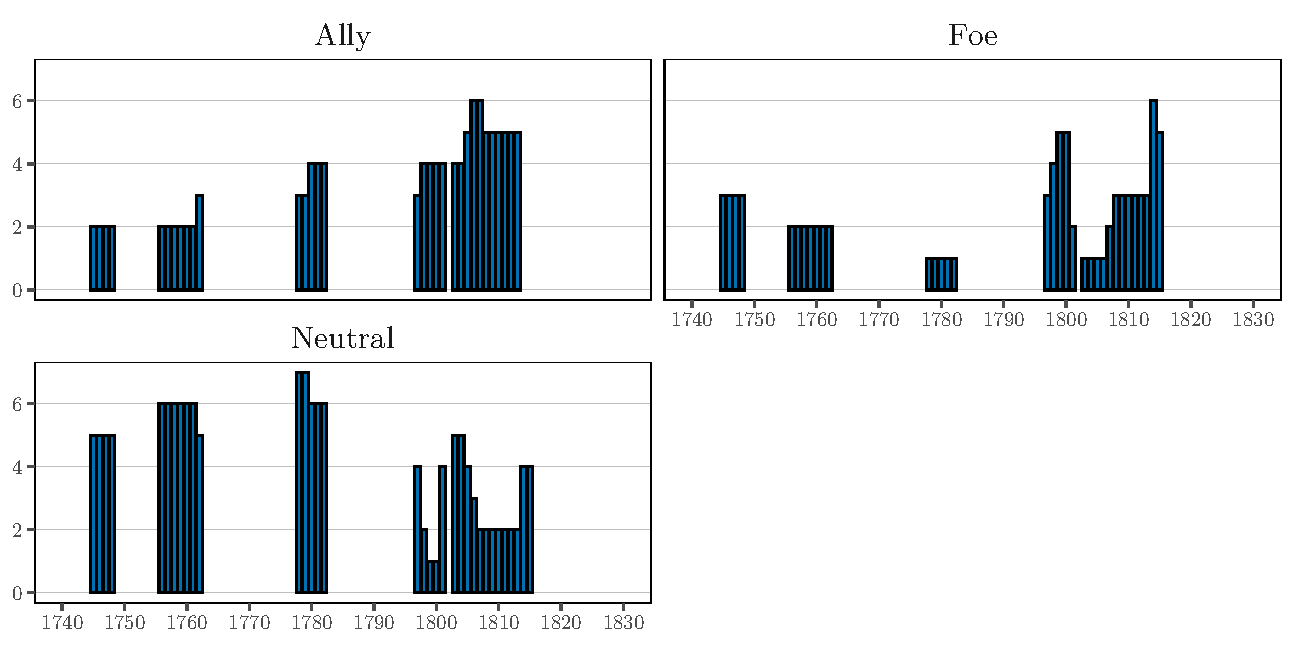
\includegraphics[scale=.8]{Number_of_protagonist.pdf}
\end{figure}
\end{center}

\begin{figure}[h!]
	\caption{Share of French trade conducted by sea}
	\centering
	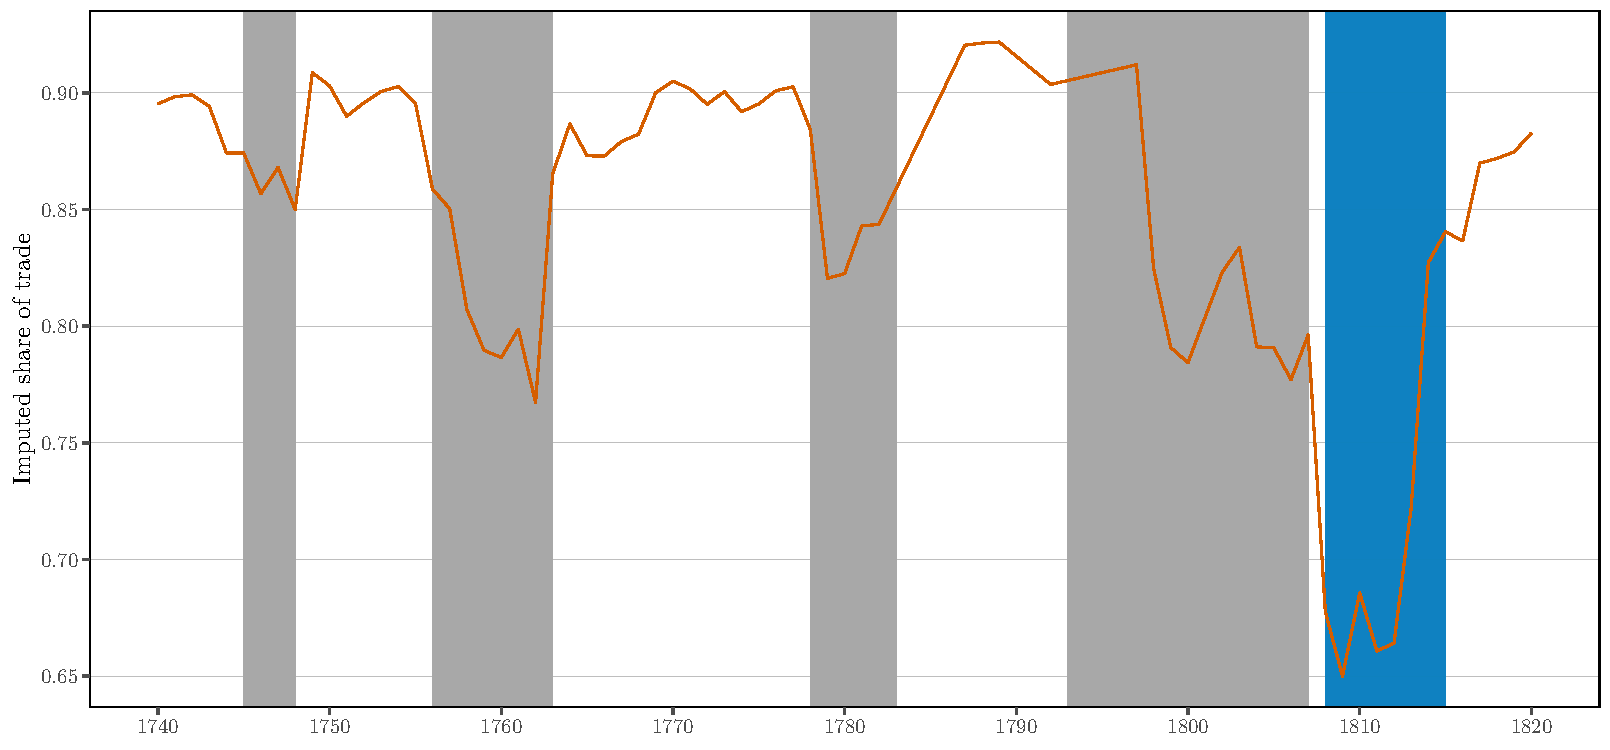
\includegraphics[scale=.7]{share_by_sea}
	\source{TOFLIT and 1792 data on the share of sea trade per country in AN F/12/1834 B}
	\label{share_by_sea}
\end{figure}


\begin{figure}[h!]
\caption{Annual and Mean Loss Function - France}
\label{fig:mean_annual_loss}
\centering
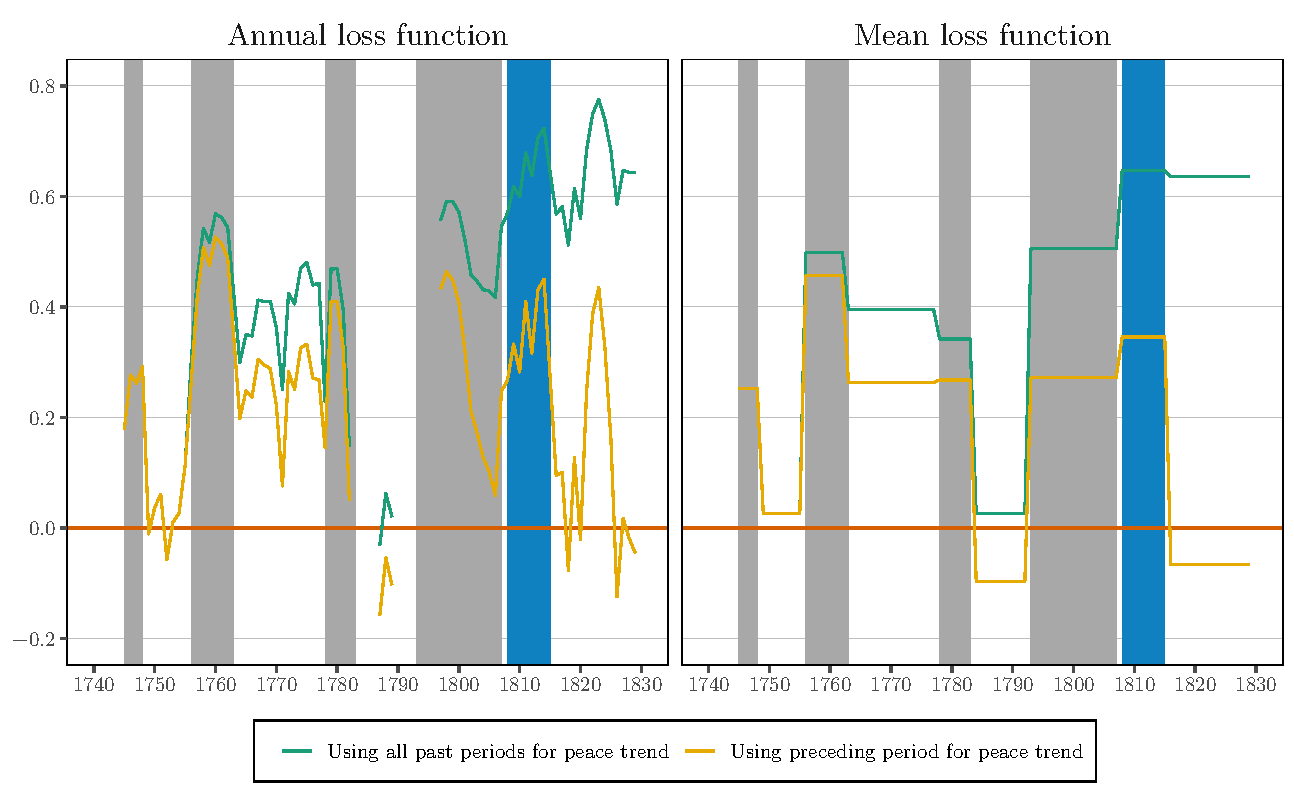
\includegraphics[scale=.7]{mean_annual_loss}
\end{figure}

\begin{figure}[h!]
\caption{Annual and Mean Loss Function - UK}
\label{fig:GBmean_annual_loss}
\centering
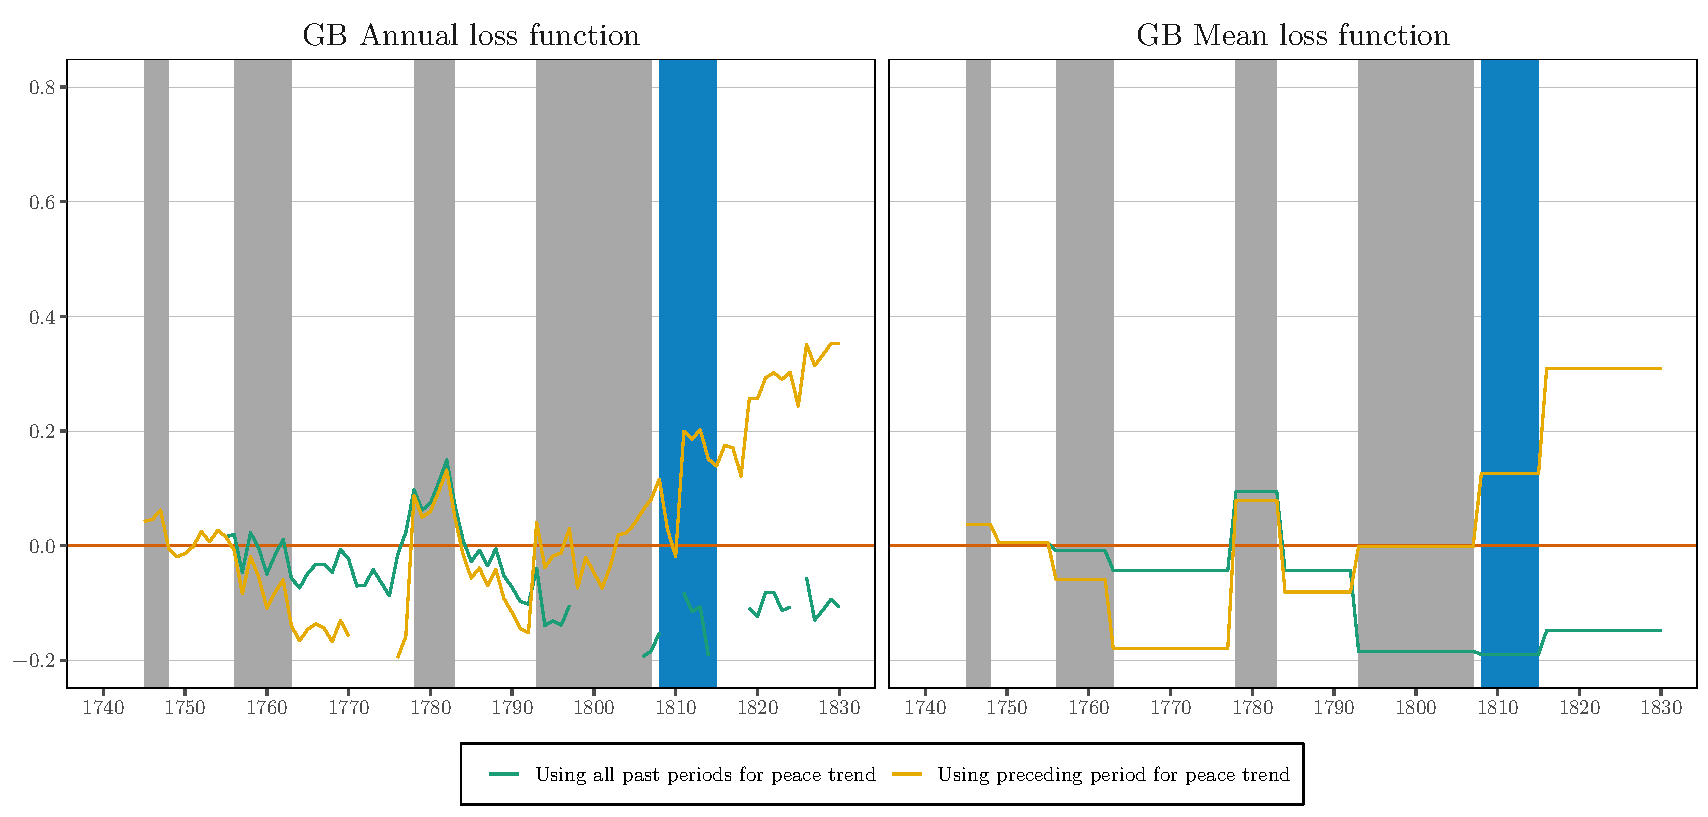
\includegraphics[scale=0.7]{GBmean_annual_loss}
\end{figure}

\begin{figure}[h!]
\caption{British Navy budget and French trade losses}
\label{Expenditures}
\centering
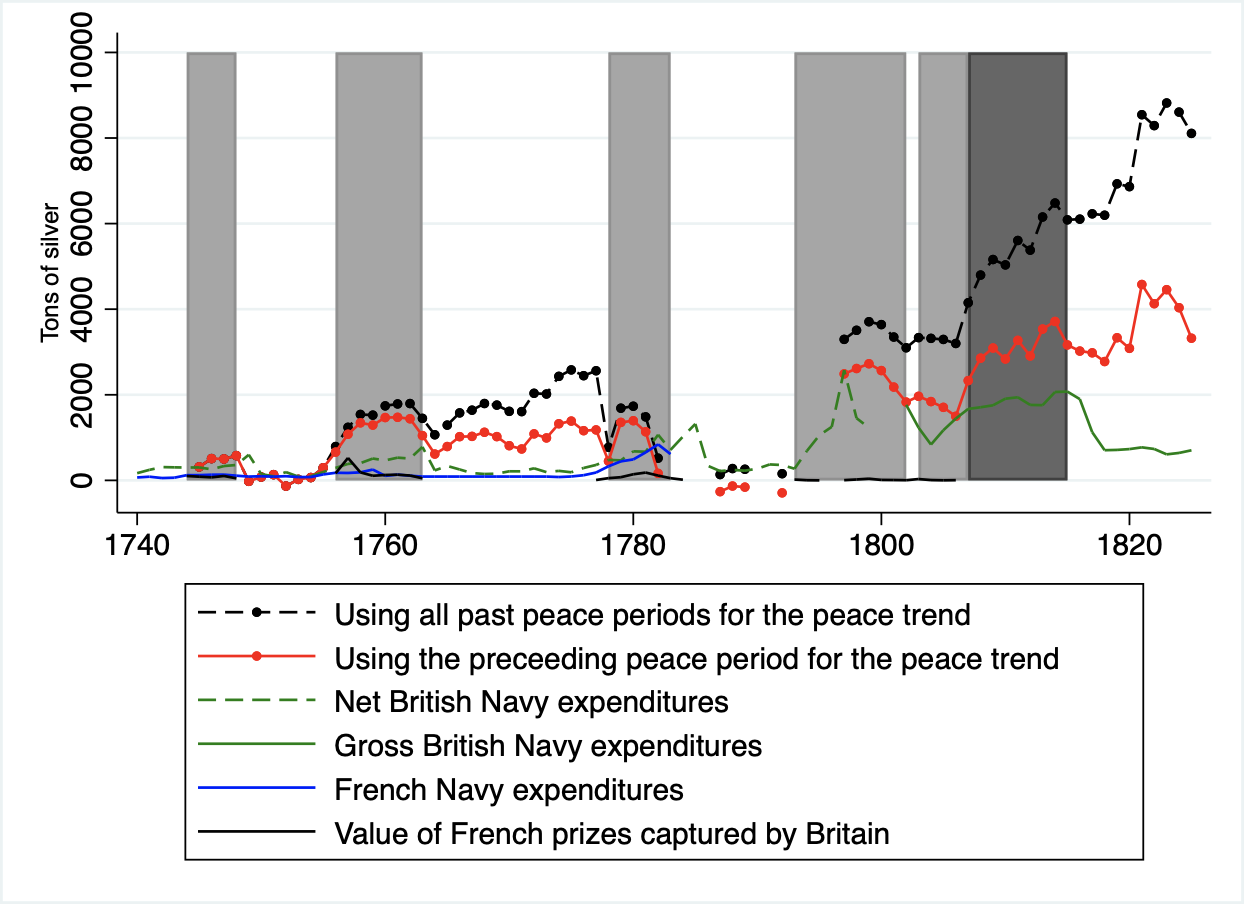
\includegraphics[scale=0.7]{Expenditures_Annual_Loss}
\source{See text and \cite[pp. 570-587]{mitchell1988}}
\end{figure}

\begin{figure}[h!]
\caption{Costs and benefits}
\label{Costs_and_benefits}
\centering
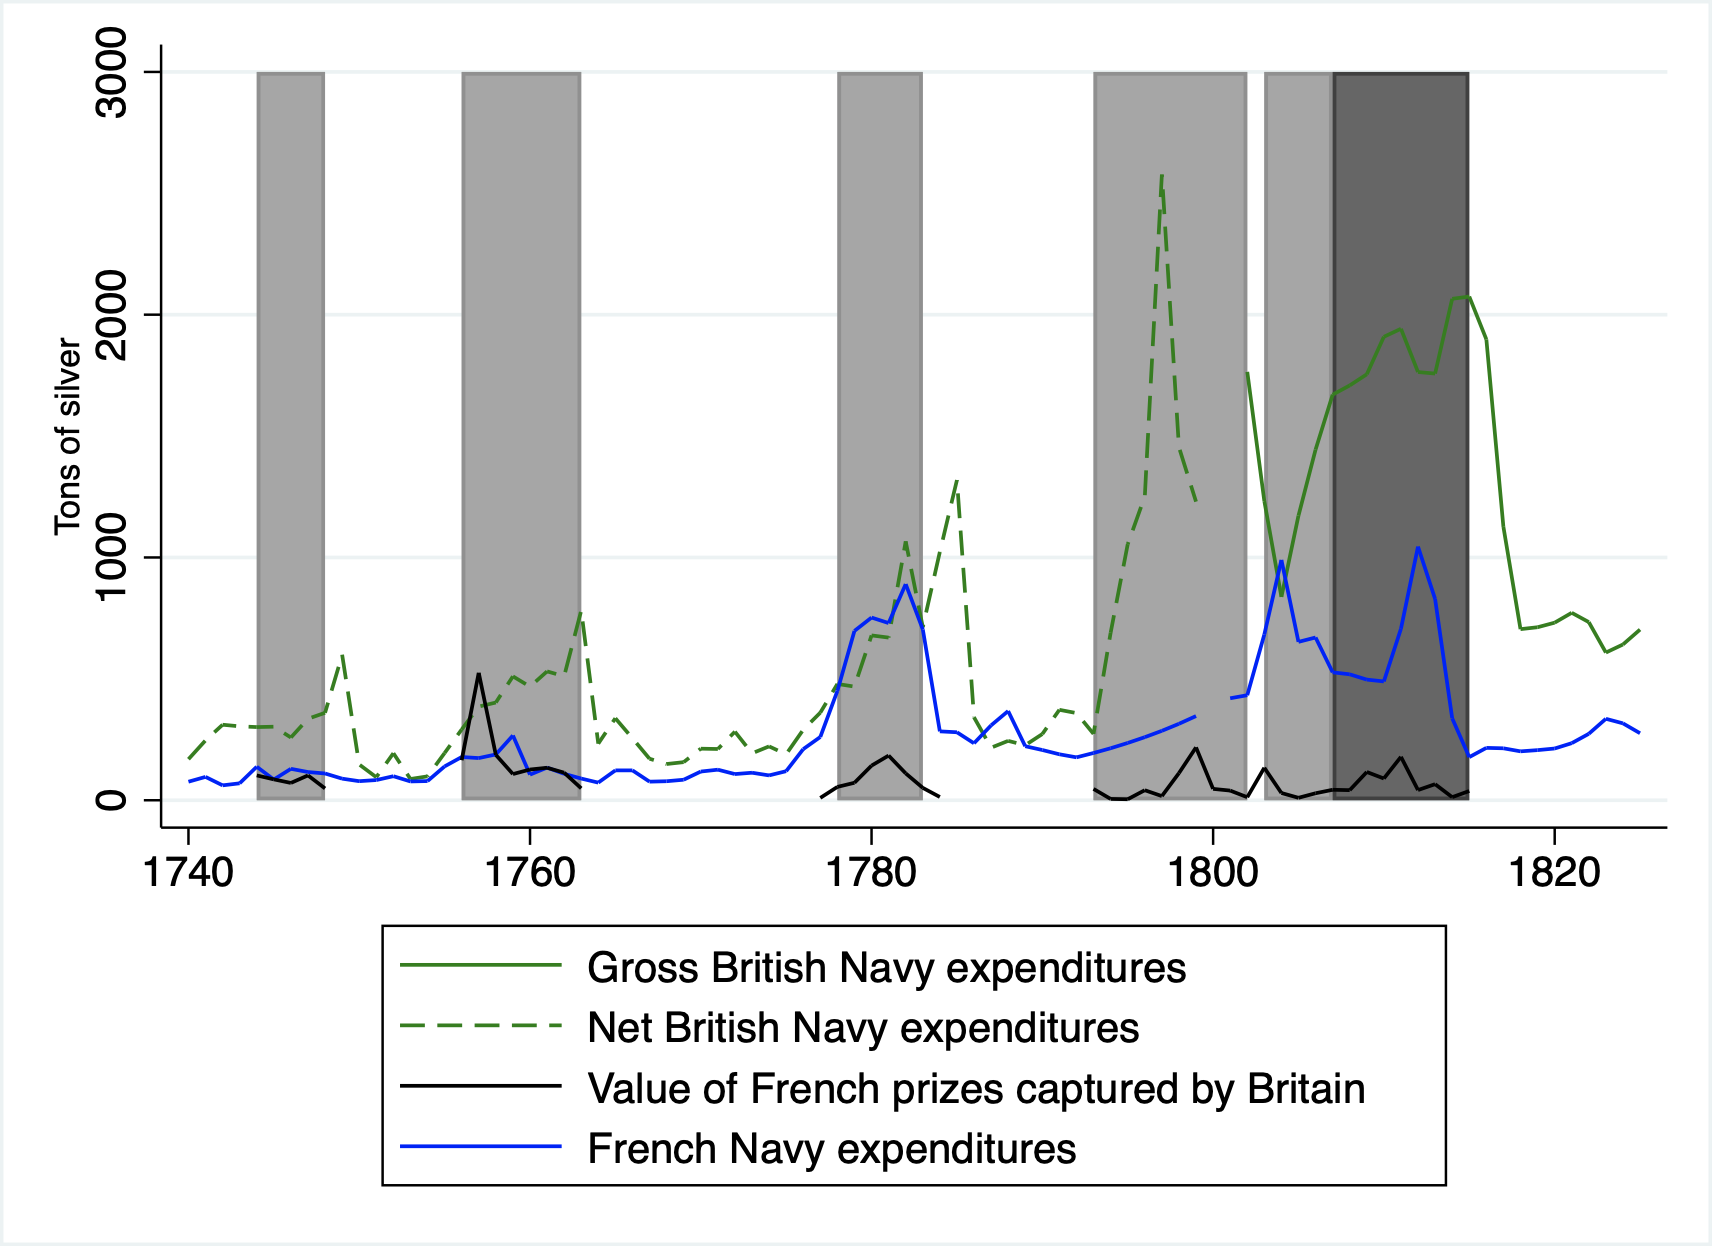
\includegraphics[scale=0.7]{Costs_and_benefits}
\end{figure}

\begin{figure}[h!]
\caption{Ratio between French trade losses and the British Navy budget, high and low hypothesis}
\label{Ratio_BR_Expenditures}
\begin{minipage}{0.9\textwidth}
\centering
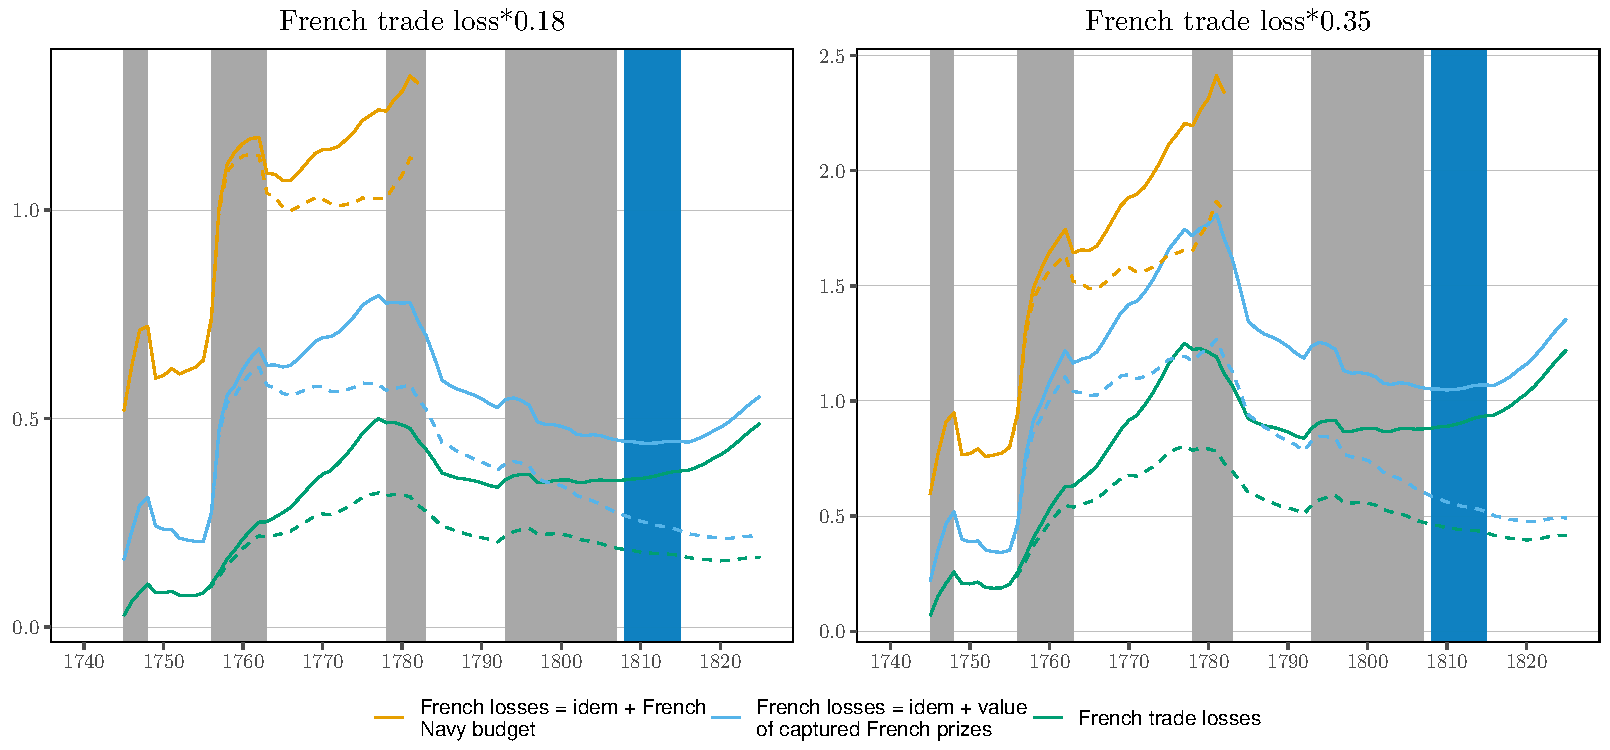
\includegraphics[scale=0.7]{ratio_BR_expenditures_ennual_loss}
\source{See text and \cite{mitchell1988}, pp. 570-587. For these graphs, French trade loss are assumed to be nil for 1783-1786, 1790-1791 and at the 1797 level for 1793-1796.}
\end{minipage}
\end{figure}

\begin{figure}[h!]
\caption{Ships captured by Great-Britain}
\label{Prizes}
\begin{minipage}{0.9\textwidth}
\centering
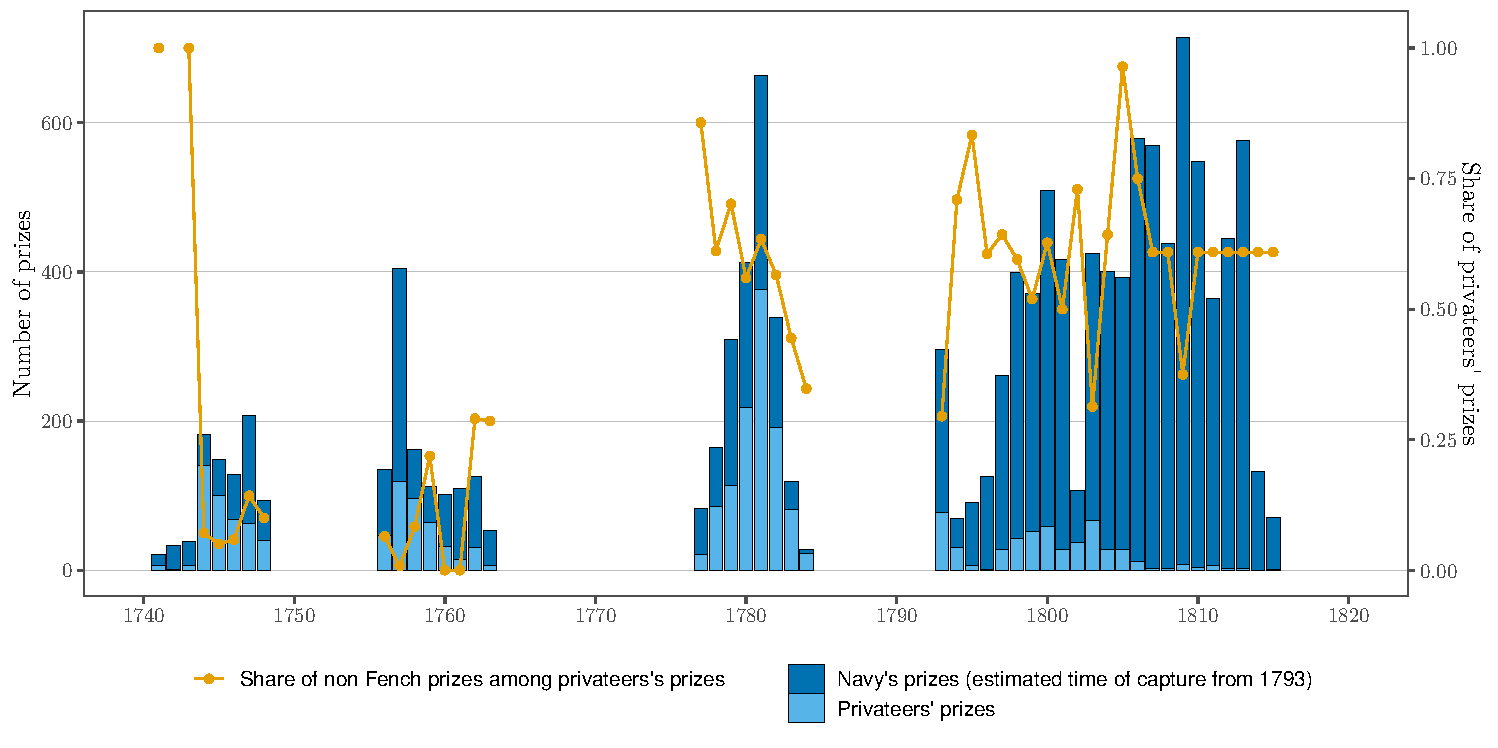
\includegraphics[scale=0.7]{Prizes}
\source{For privateers and before 1785 for the Royal Navy, \cite{Starkey1990,Hillmann2011}. For post-1793 Royal Navy prizes, we use the data on the value of Navy Prizes from \cite{Benjamin2009}, based on \cite{Hill1998}.}
\end{minipage}
\end{figure}

\begin{figure}[h!]
\caption{Prize goods imports in Great-Britain}
\label{Prize goods imports}
\centering
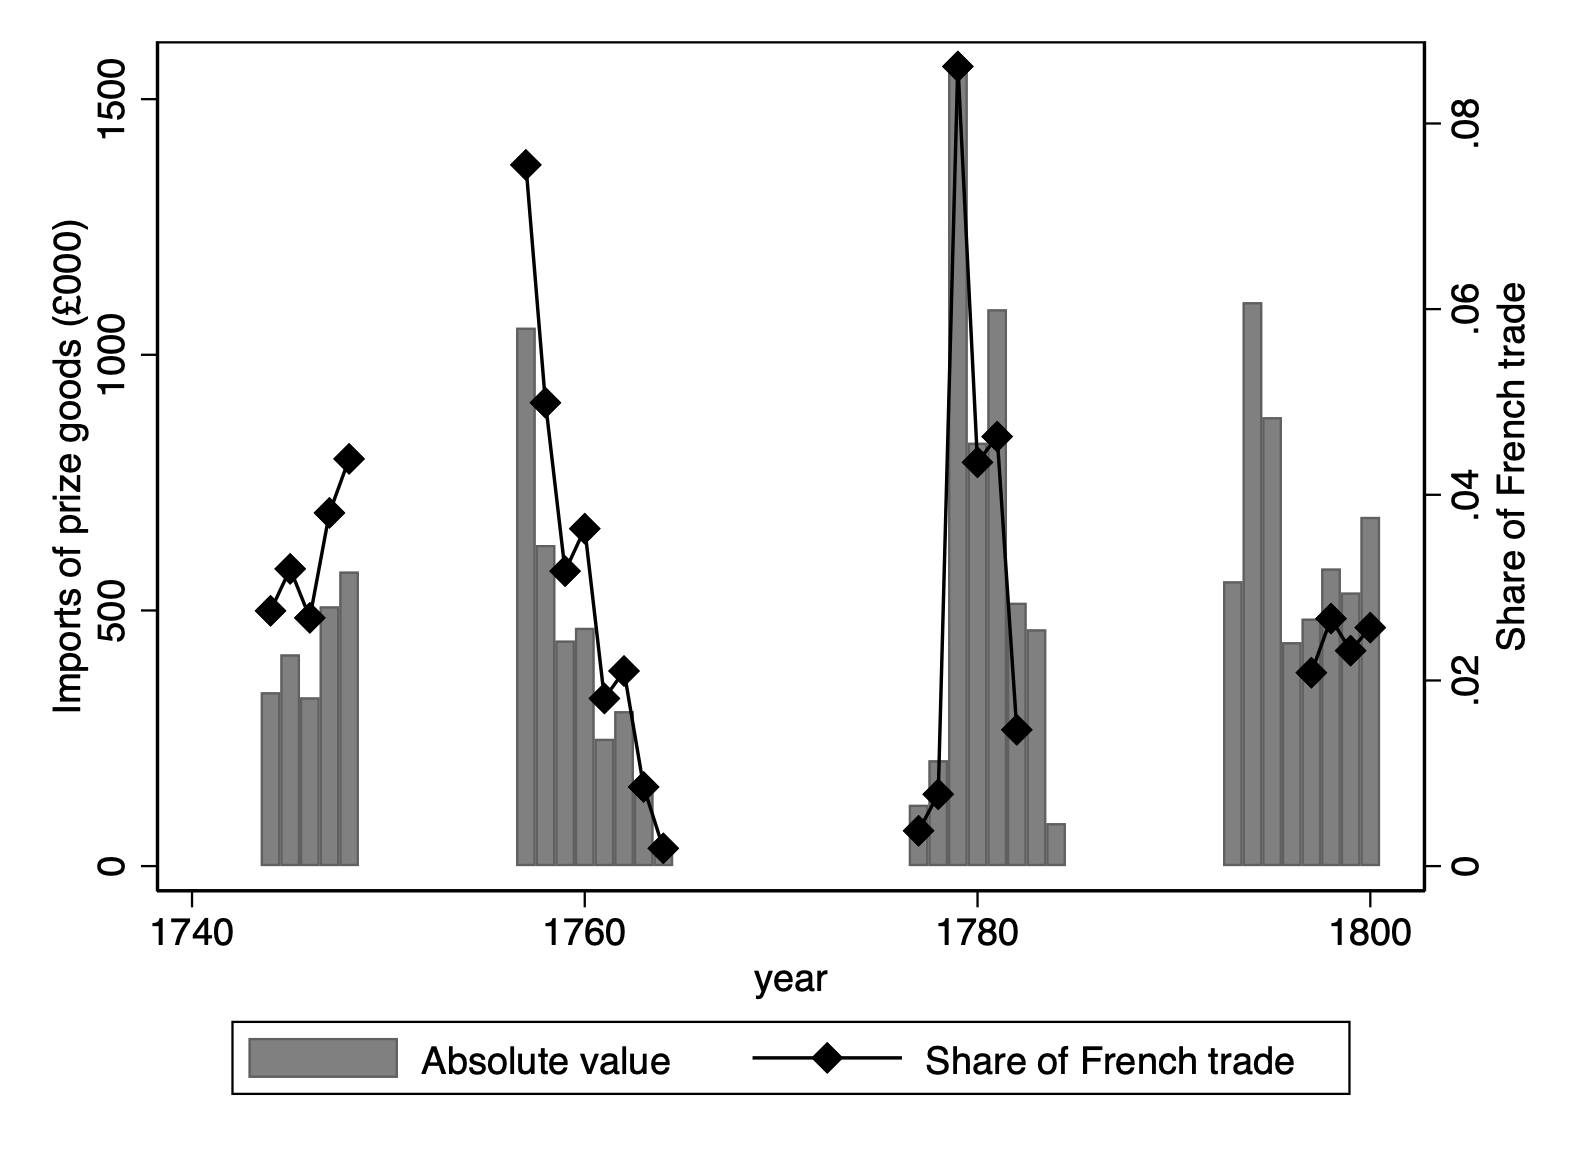
\includegraphics[scale=0.7]{Prizes_imports}
\source{\cite{Ashton1960}}
\end{figure}

\begin{figure}[h!]
\caption{Naval Supremacy Ratio}
\label{naval_supremacy_ratios}
\centering
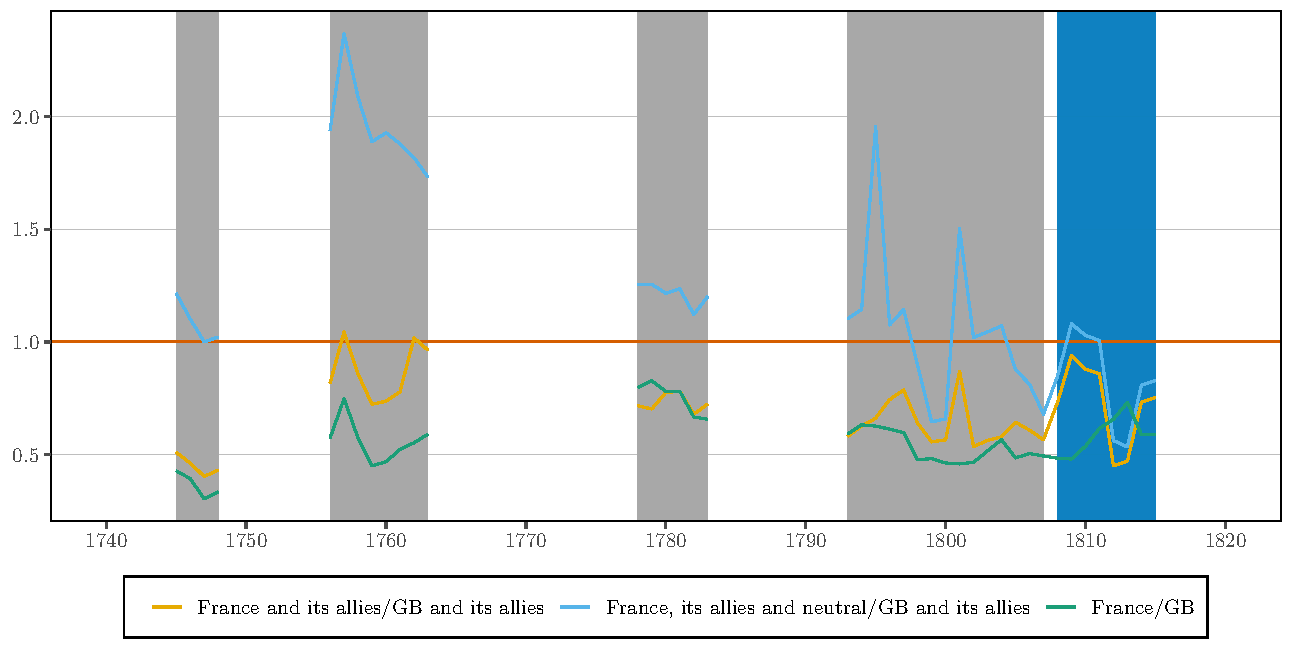
\includegraphics[scale=.7]{naval_supremacy_ratio}
\end{figure}

\begin{figure}[h!]
\caption{Colonial empire loss}
\label{colony_loss}
\centering
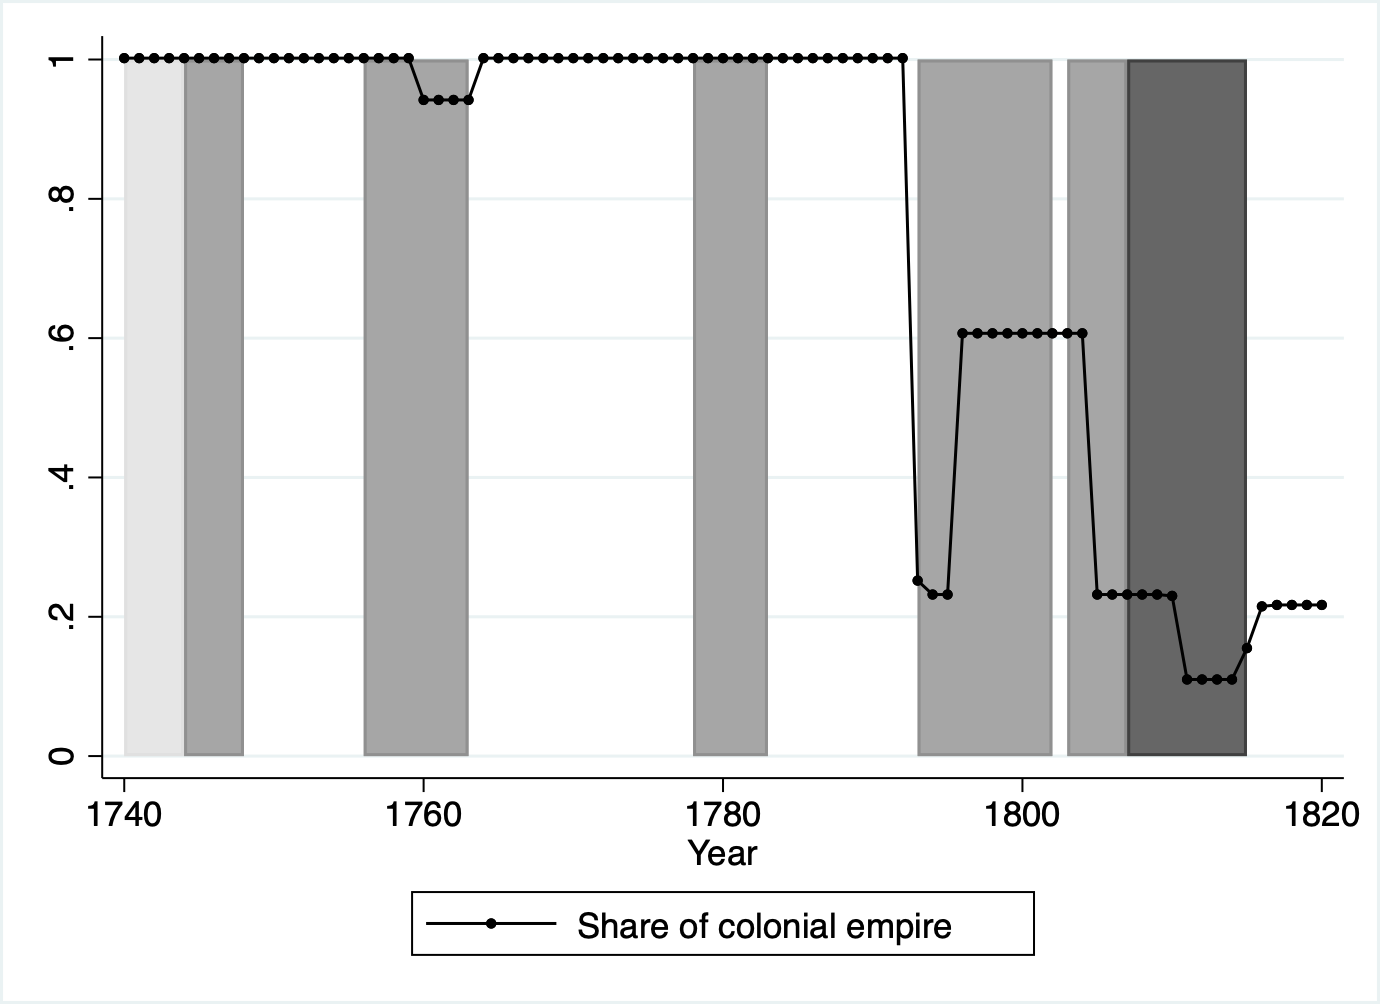
\includegraphics[scale=.8]{colony_loss}
\end{figure}

\begin{figure}[h!]
\caption{Nationality of non-French British prizes}
\label{fig:prizes_nationality}
\begin{minipage}{0.9\textwidth}
\centering
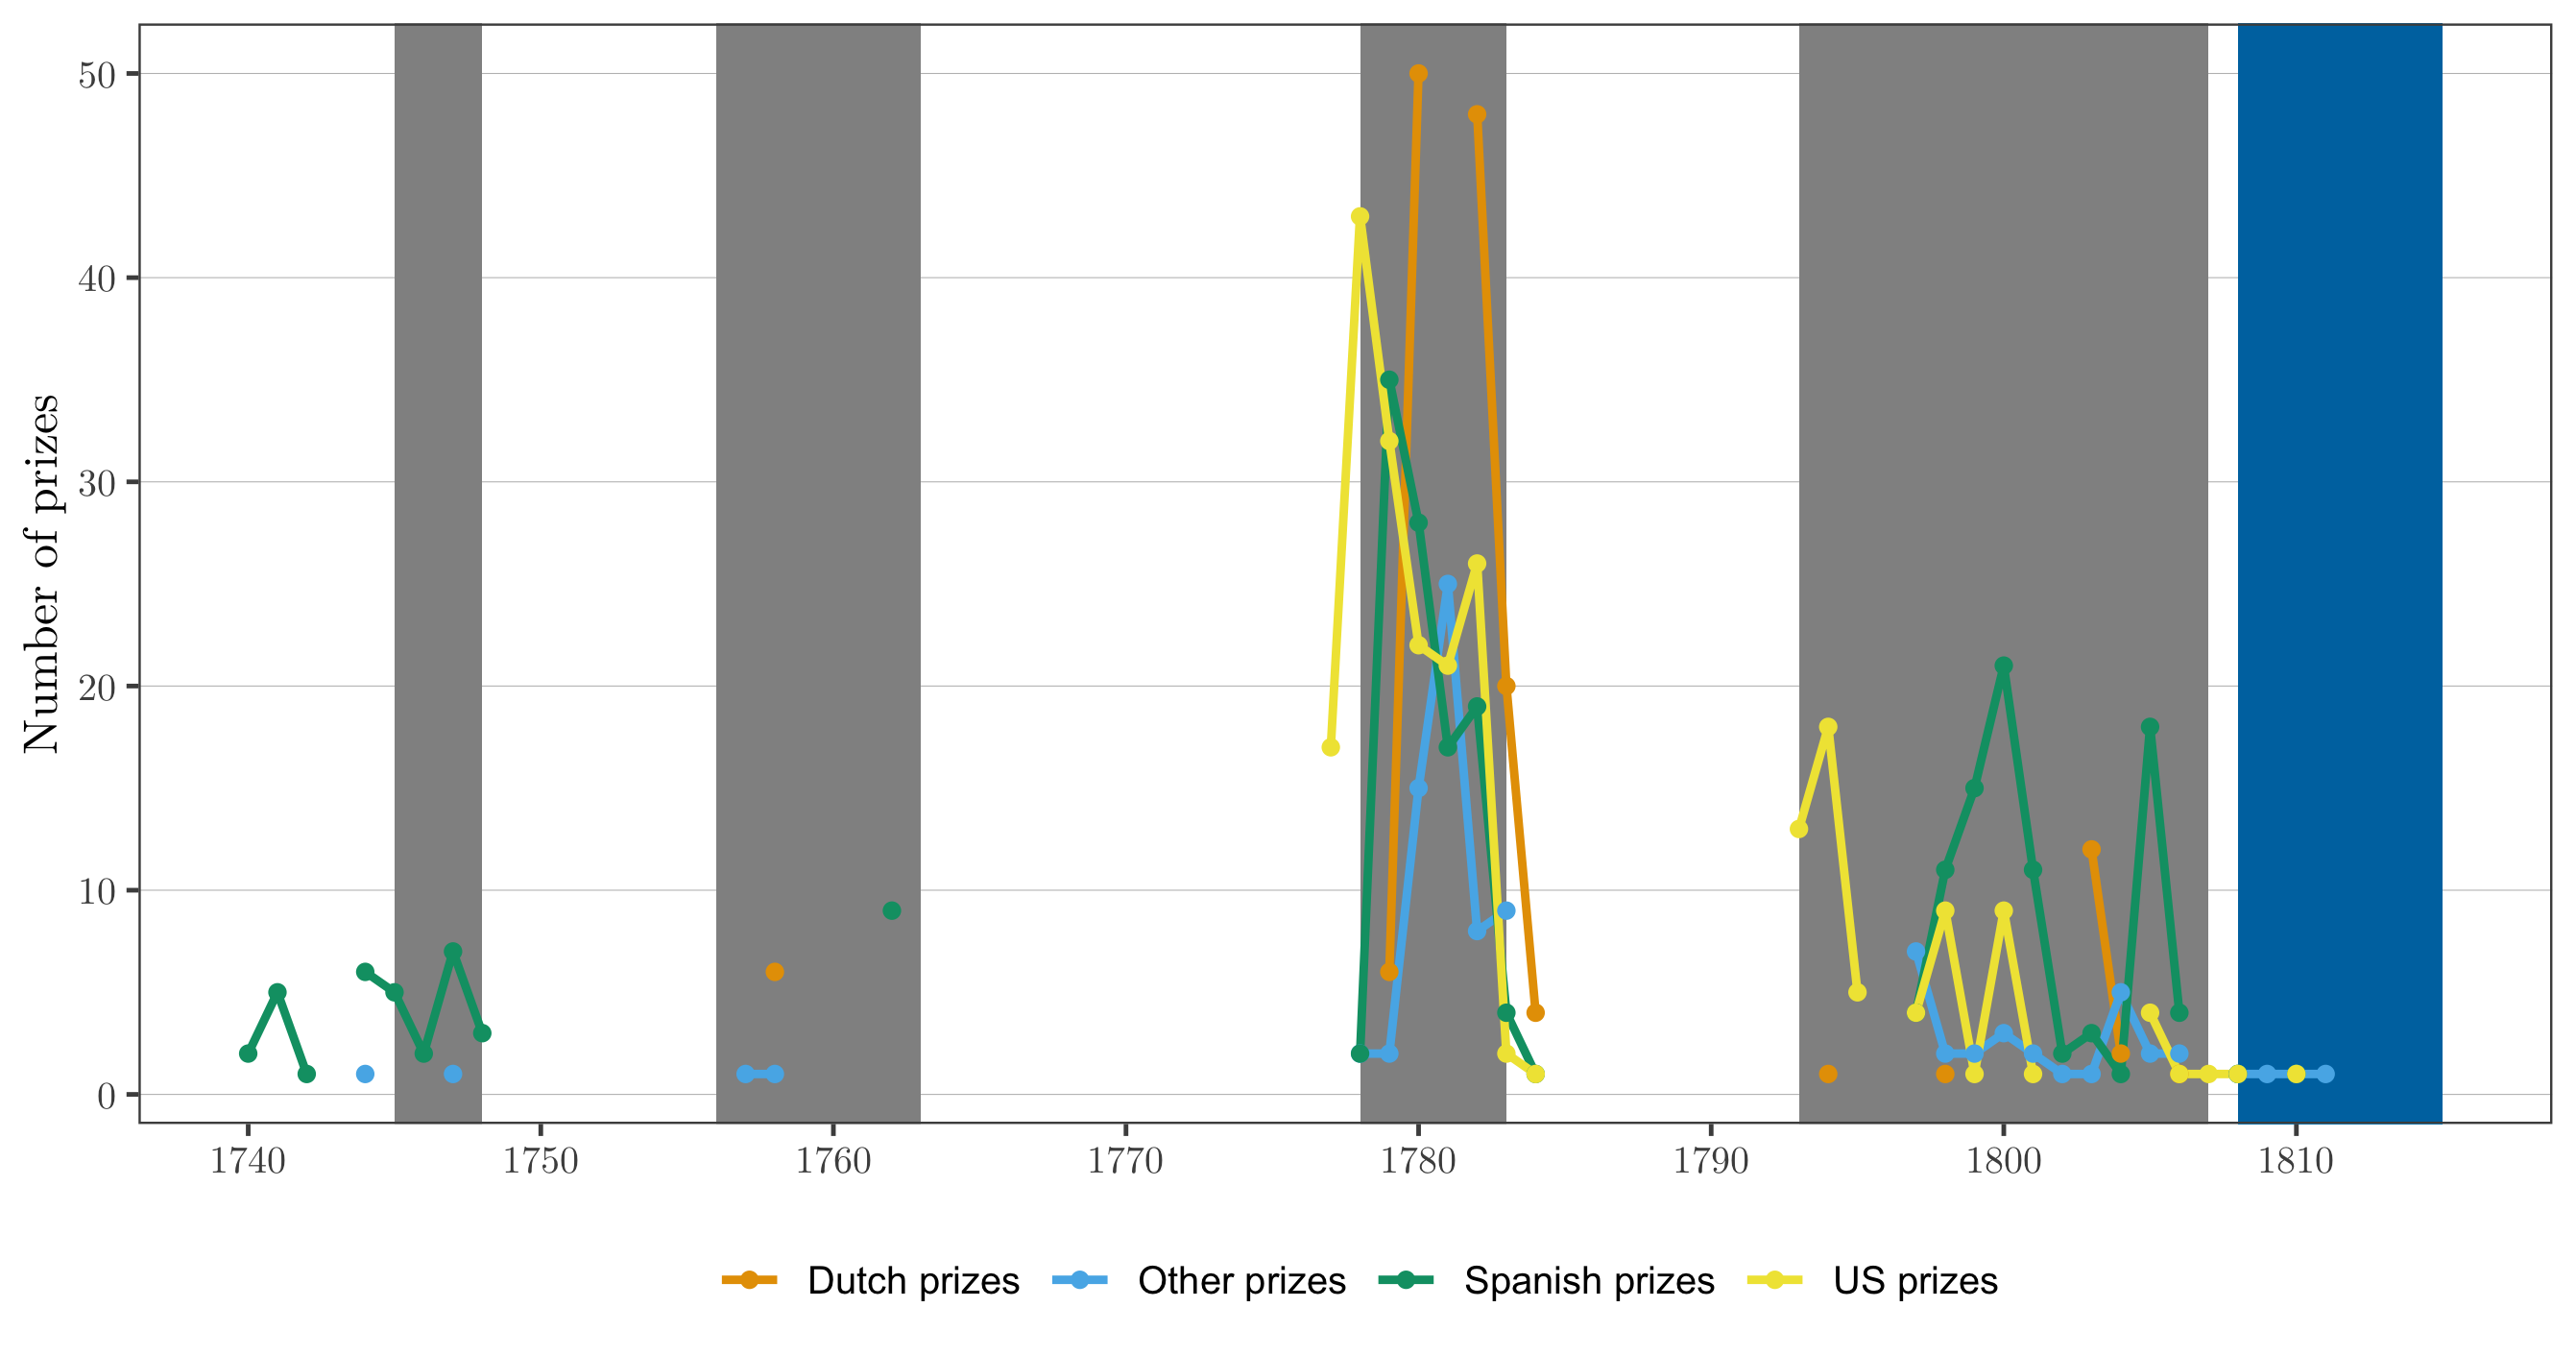
\includegraphics[scale=.8]{Prizes_nationality}
\source{For privateers and before 1785 for the Royal Navy, \cite{Starkey1990} and \cite{Hillmann2011}. For post-1793 Royal Navy prizes, we use the data on the value of Navy Prizes from \cite{Benjamin2009}, based on \cite{Hill1998}. The peak in Dutch prices in 1781 is omitted in this figure for readability. \todo[inline, color = YellowGreen]{Why was there the peak?? I cant remember anymore. Also what is the y axis here? -- The peak comes from the beginning of the 4th Anglo-Dutch War. I am not sure it should be omitted : it is an important fact.Maybe cut the Y axis ? This kind of stuff ? https://www.extendoffice.com/documents/excel/2716-excel-chart-break-axis.html  Some of these Dutch guys were doing French trave, obviously. Y-axis is the number of prizes}}
\end{minipage}
\end{figure}

\begin{center}
\begin{figure}[h!]
\centering
\caption{Trade loss by war status - Total trade}
\label{fig:loss_by_war_status_XI}
\begin{minipage}{.95\textwidth}
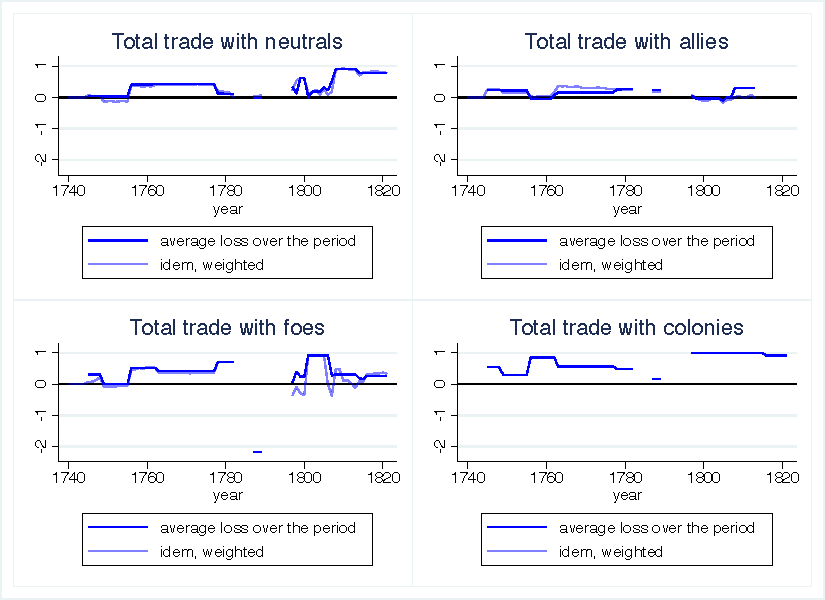
\includegraphics[scale=.7]{loss_by_war_status_XI}
\source{This figure is constructed by computing the mean country-specific trade loss function by war status based on all preceding peace periods.
We have both a trade-weighted measure and a non-trade weighted measure, where we had to exclude \textit{Empereur} after 1794, because of a territorial change- trade was mainly with current Belgium before 1794 and mainly with Austria after 1794 - and \textit{Hollande} after 1814 as it included current day Belgium from 1815.
The negative trade loss number for trade with foes in 1787-1789 can be explained by the large effect of the Eden treaty.}
\end{minipage}
\end{figure}
\end{center}

\begin{center}
\begin{figure}[h!]
\centering
\caption{Trade loss by war status}
\label{fig:loss_by_war_status_X_I}
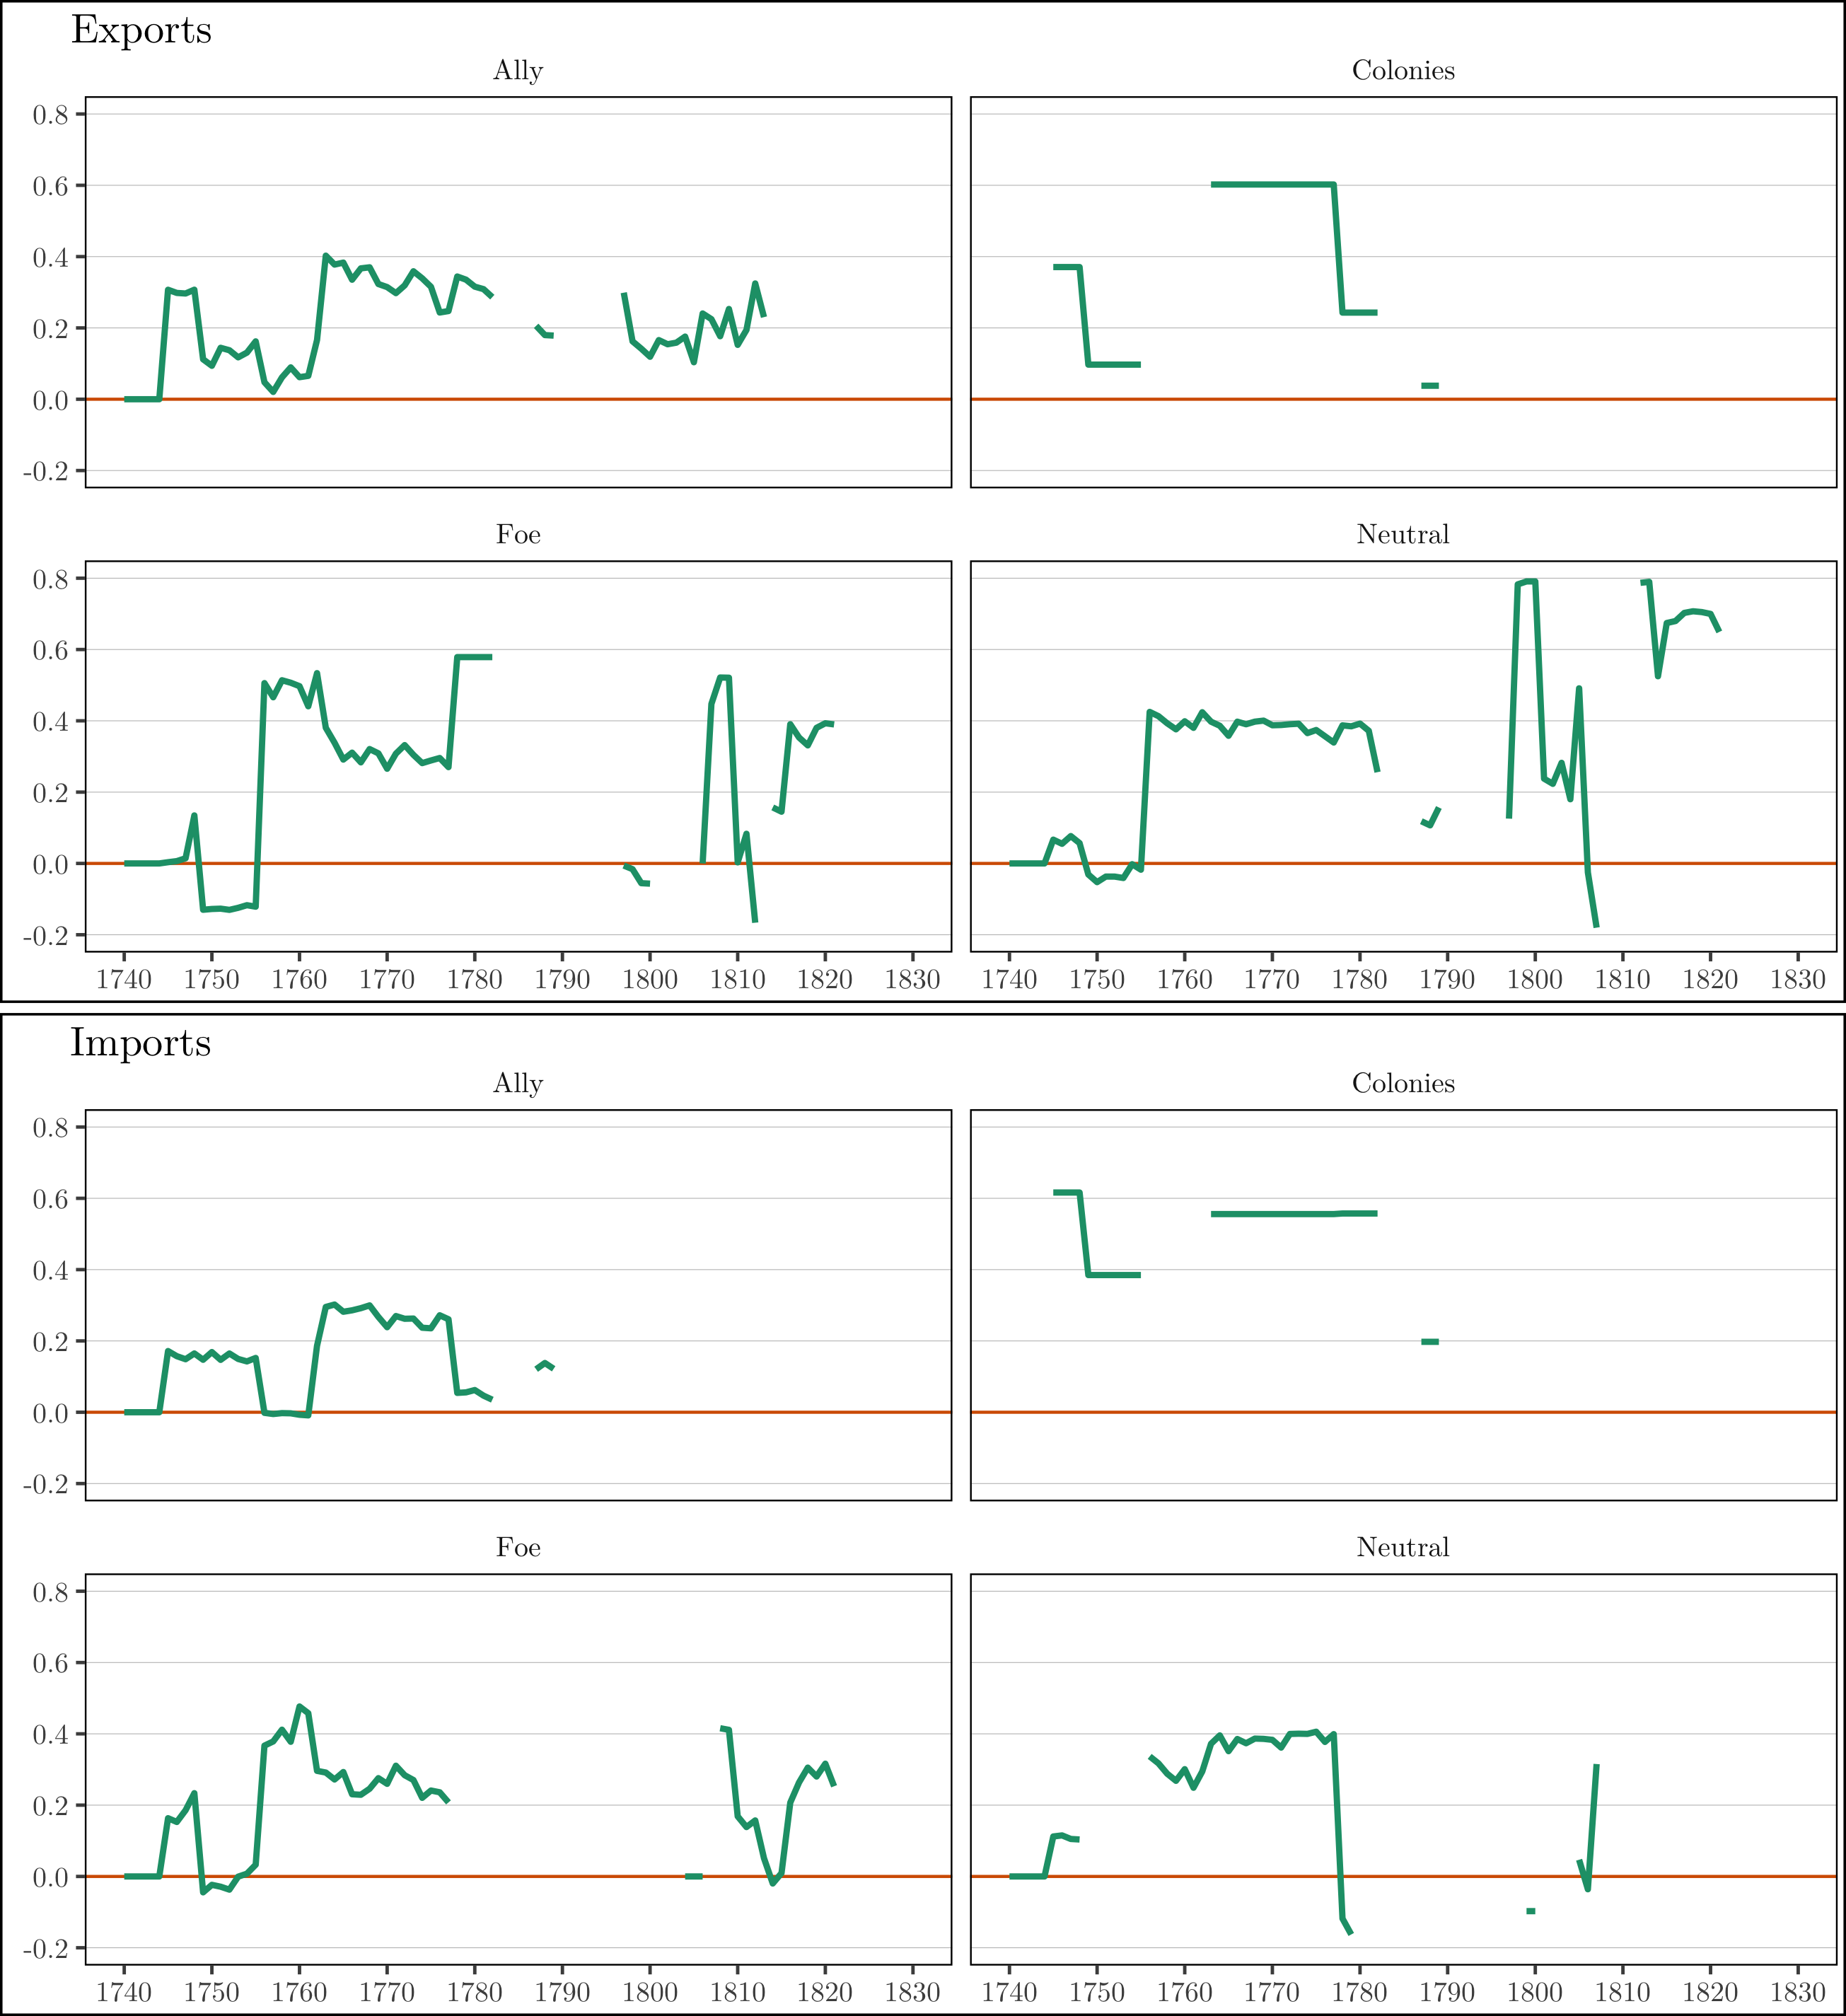
\includegraphics[scale=.8]{loss_by_war_status_X_I_combined}
\end{figure}
\end{center}



% This code uses the tikz package

\begin{center}
	\begin{figure}[h!]
		\centering
		\caption{Directed acyclical graphs (DAG) of causality between war and peacetime losses (\cite{Pearl2000,Pearl2018,Schneider2020})}
		\label{DAG}
		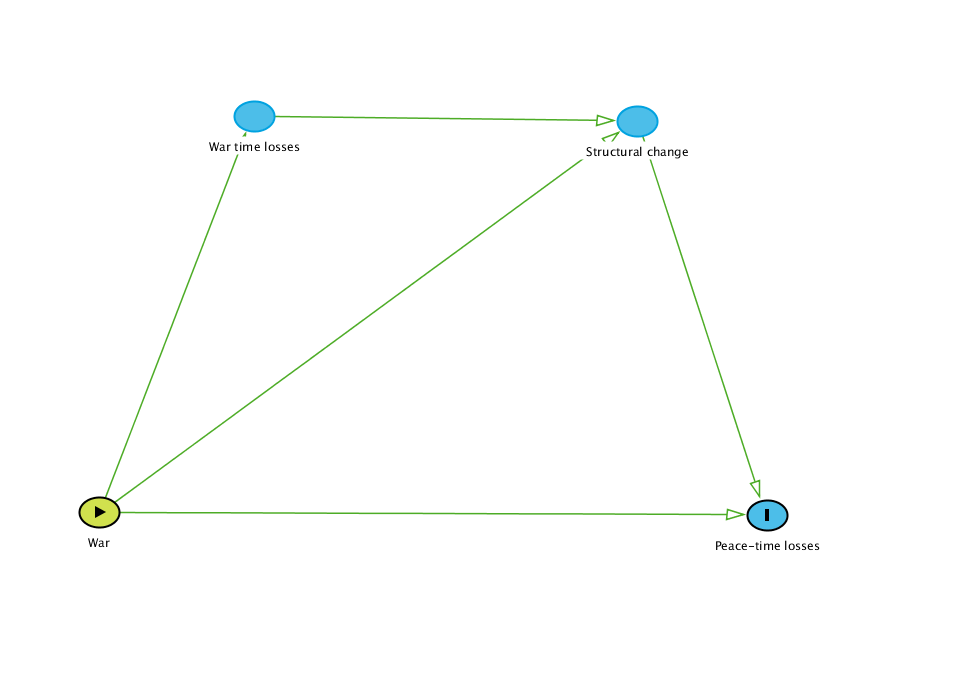
\includegraphics[scale=0.8]{dagitty-model-War-to-PeaceTimeLosses.png}
	\end{figure}


	\begin{figure}[h!]
	\centering
	\caption{Directed acyclical graphs (DAG) of causality between war and peacetime losses (\cite{Pearl2000,Pearl2018,Schneider2020})}
	\label{DAG}
	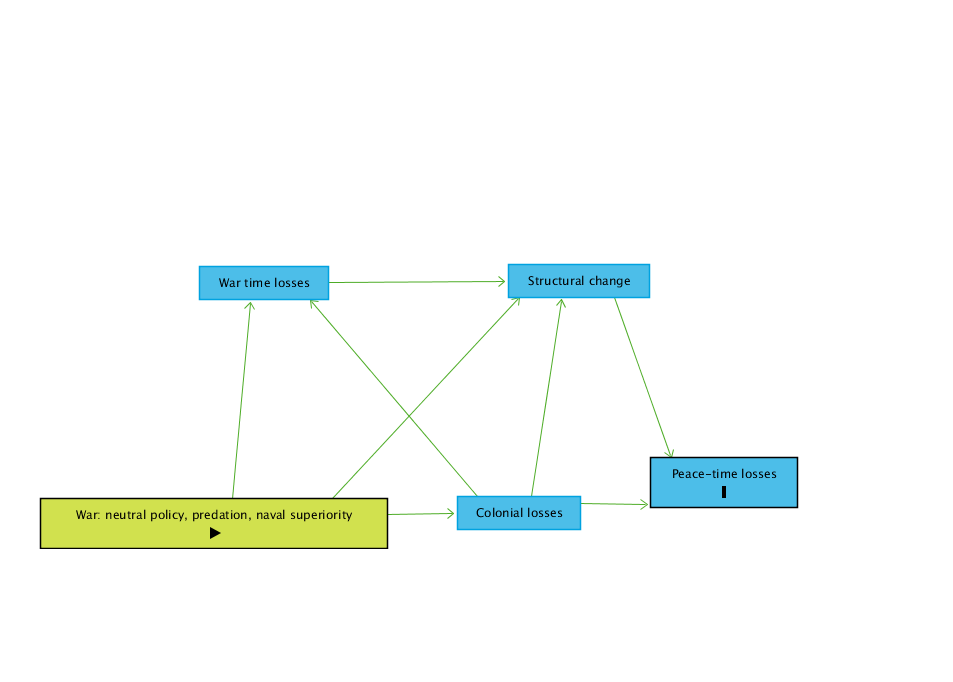
\includegraphics[scale=0.8]{dagitty-model-War-to-PeaceTimeLosses-othergo.png}
\end{figure}
\end{center}

\begin{tikzpicture}
	\node (v0) at (0,0) {War};
	\node (v1) at (10,0) {Peace-time losses};
	\node (v2) at (-0,5) {War time losses};
	\node (v3) at (5,5) {Structural change};
	\draw [->] (v0) edge (v2);
	\draw [->] (v2) edge (v3);
	\draw [->] (v3) edge (v1);
	\draw [->] (v0) edge (v3);
	\draw [->] (v0) edge (v1);
\end{tikzpicture}



\begin{landscape}
\begin{table}[h!]
	\caption{Regression of the various the loss functions on the log of sectorial shares of exports (N=54)}
	\label{Individual_regressions_sector_exports}
	\footnotesize
	\def\sym#1{\ifmmode^{#1}\else\(^{#1}\)\fi}
\begin{tabular}{p{1.5cm} p{1.7cm} p{1.7cm} p{1.7cm} p{1.7cm} p{1.7cm} p{1.7cm} p{1.7cm} p{1.7cm} p{1.7cm} p{1.7cm} p{1.7cm} p{1.7cm}}
                &\multicolumn{1}{c}{\shortstack{Other\\foodstuff}"}&\multicolumn{1}{c}{\shortstack{Plantation\\foodstuff}}&\multicolumn{1}{c}{\shortstack{Drinks\\and\\tobacco}}&\multicolumn{1}{c}{\shortstack{Crude\\material}}&\multicolumn{1}{c}{Oils}&\multicolumn{1}{c}{\shortstack{Chemical\\products}}&\multicolumn{1}{c}{\shortstack{Leather\\wood and\\paper\\products}}&\multicolumn{1}{c}{\shortstack{Other\\threads\\and fabric}}&\multicolumn{1}{c}{\shortstack{Wool\\threads\\and fabrics}}&\multicolumn{1}{c}{\shortstack{Silk\\threads\\and fabrics}}&\multicolumn{1}{c}{\shortstack{Cotton\\threads\\and fabrics}}&\multicolumn{1}{c}{\shortstack{Other\\industrial\\products}}\\
\hline
loss            &   -0.244         &   -3.848\sym{**} &    0.376         &   -0.884\sym{***}&    0.235         &   -0.510         &    0.789\sym{***}&    0.020         &    2.044\sym{***}&    1.371\sym{***}&   -0.789         &    0.714\sym{**} \\
                &  (-1.04)         &  (-3.49)         &   (1.68)         &  (-3.72)         &   (0.66)         &  (-1.60)         &   (3.59)         &   (0.07)         &   (5.01)         &   (8.24)         &  (-1.98)         &   (3.43)         \\
year            &    0.013\sym{***}&   -0.043\sym{***}&    0.007\sym{***}&    0.023\sym{***}&    0.017\sym{***}&   -0.004         &    0.007\sym{***}&   -0.009\sym{**} &   -0.029\sym{***}&    0.002         &    0.020\sym{***}&    0.001         \\
                &   (6.51)         &  (-4.43)         &   (3.66)         &  (10.96)         &   (5.54)         &  (-1.28)         &   (3.53)         &  (-3.39)         &  (-8.07)         &   (1.18)         &   (5.74)         &   (0.52)         \\
\end{tabular}
\def\sym#1{\ifmmode^{#1}\else\(^{#1}\)\fi}
\begin{tabular}{p{1.5cm} p{1.7cm} p{1.7cm} p{1.7cm} p{1.7cm} p{1.7cm} p{1.7cm} p{1.7cm} p{1.7cm} p{1.7cm} p{1.7cm} p{1.7cm} p{1.7cm}}
\hline
loss\_nm         &   -0.089         &   -4.143\sym{***}&    0.413         &   -0.829\sym{***}&    0.363         &   -0.537         &    0.923\sym{***}&    0.235         &    1.759\sym{***}&    1.315\sym{***}&   -0.728         &    0.732\sym{***}\\
                &  (-0.39)         &  (-4.06)         &   (1.95)         &  (-3.63)         &   (1.08)         &  (-1.77)         &   (4.69)         &   (0.81)         &   (4.31)         &   (8.31)         &  (-1.91)         &   (3.74)         \\
year            &    0.012\sym{***}&   -0.048\sym{***}&    0.008\sym{***}&    0.021\sym{***}&    0.017\sym{***}&   -0.004         &    0.008\sym{***}&   -0.010\sym{***}&   -0.024\sym{***}&    0.004\sym{**} &    0.019\sym{***}&    0.002         \\
                &   (6.80)         &  (-5.88)         &   (4.50)         &  (11.54)         &   (6.33)         &  (-1.78)         &   (4.80)         &  (-4.27)         &  (-7.42)         &   (3.35)         &   (6.03)         &   (1.32)         \\
\end{tabular}
\def\sym#1{\ifmmode^{#1}\else\(^{#1}\)\fi}
\begin{tabular}{p{1.5cm} p{1.7cm} p{1.7cm} p{1.7cm} p{1.7cm} p{1.7cm} p{1.7cm} p{1.7cm} p{1.7cm} p{1.7cm} p{1.7cm} p{1.7cm} p{1.7cm}}
\hline
ln(loss)        &   -0.085         &   -0.655\sym{*}  &    0.094         &   -0.222\sym{***}&    0.049         &   -0.076         &    0.153\sym{**} &    0.029         &    0.401\sym{***}&    0.274\sym{***}&   -0.310\sym{***}&    0.088         \\
                &  (-1.64)         &  (-2.54)         &   (1.90)         &  (-4.33)         &   (0.62)         &  (-1.05)         &   (3.02)         &   (0.42)         &   (4.17)         &   (6.58)         &  (-3.82)         &   (1.75)         \\
year            &    0.014\sym{***}&   -0.054\sym{***}&    0.008\sym{***}&    0.022\sym{***}&    0.018\sym{***}&   -0.005\sym{*}  &    0.009\sym{***}&   -0.010\sym{***}&   -0.024\sym{***}&    0.005\sym{**} &    0.021\sym{***}&    0.004\sym{*}  \\
                &   (7.61)         &  (-6.04)         &   (4.52)         &  (12.32)         &   (6.51)         &  (-2.10)         &   (4.99)         &  (-4.05)         &  (-7.30)         &   (3.37)         &   (7.50)         &   (2.06)         \\
\end{tabular}
\def\sym#1{\ifmmode^{#1}\else\(^{#1}\)\fi}
\begin{tabular}{p{1.5cm} p{1.7cm} p{1.7cm} p{1.7cm} p{1.7cm} p{1.7cm} p{1.7cm} p{1.7cm} p{1.7cm} p{1.7cm} p{1.7cm} p{1.7cm} p{1.7cm}}
\hline
ln(loss\_nm)     &   -0.034         &   -0.726\sym{***}&    0.086\sym{*}  &   -0.186\sym{***}&    0.074         &   -0.085         &    0.166\sym{***}&    0.046         &    0.345\sym{***}&    0.252\sym{***}&   -0.217\sym{**} &    0.114\sym{**} \\
                &  (-0.80)         &  (-3.61)         &   (2.13)         &  (-4.44)         &   (1.14)         &  (-1.45)         &   (4.27)         &   (0.82)         &   (4.43)         &   (8.21)         &  (-3.12)         &   (2.91)         \\
year            &    0.013\sym{***}&   -0.053\sym{***}&    0.008\sym{***}&    0.021\sym{***}&    0.017\sym{***}&   -0.005\sym{*}  &    0.009\sym{***}&   -0.010\sym{***}&   -0.023\sym{***}&    0.005\sym{***}&    0.019\sym{***}&    0.003\sym{*}  \\
                &   (7.34)         &  (-6.66)         &   (4.94)         &  (12.61)         &   (6.79)         &  (-2.19)         &   (5.60)         &  (-4.42)         &  (-7.41)         &   (4.50)         &   (6.95)         &   (2.04)         \\
\end{tabular}

	\source{The log of "negative" losses is replaces by the log of the minimum loss in the data}
\end{table}

\begin{table}[h!]
	\caption{Regression the loss functions on the log of the sectorial shares of imports(N=54)}
	\label{Individual_regressions_sector_imports}
	\footnotesize
	\def\sym#1{\ifmmode^{#1}\else\(^{#1}\)\fi}
\begin{tabular}{p{1.5cm} p{1.7cm} p{1.7cm} p{1.7cm}  p{1.7cm} p{1.7cm} p{1.7cm} p{1.7cm} p{1.7cm}  p{1.7cm} p{1.7cm} p{1.7cm} p{1.7cm} }
                &\multicolumn{1}{c}{\shortstack{Other\\foodstuff}"}&\multicolumn{1}{c}{\shortstack{Plantation\\foodstuff}}&\multicolumn{1}{c}{\shortstack{Drinks\\and\\tobacco}}&\multicolumn{1}{c}{\shortstack{Crude\\material}}&\multicolumn{1}{c}{Oils}&\multicolumn{1}{c}{\shortstack{Chemical\\products}}&\multicolumn{1}{c}{\shortstack{Leather\\wood and\\paper\\products}}&\multicolumn{1}{c}{\shortstack{Other\\threads\\and fabric}}&\multicolumn{1}{c}{\shortstack{Wool\\threads\\and fabrics}}&\multicolumn{1}{c}{\shortstack{Silk\\threads\\and fabrics}}&\multicolumn{1}{c}{\shortstack{Cotton\\threads\\and fabrics}}&\multicolumn{1}{c}{\shortstack{Other\\industrial\\products}}\\
\hline
loss            &   -0.173         &   -1.764\sym{*}  &   -0.277         &    0.140         &    0.324         &    0.630\sym{*}  &    1.499\sym{**} &    0.466         &    2.585\sym{**} &    2.189         &   -2.295         &    0.431         \\
                &  (-0.42)         &  (-2.34)         &  (-0.44)         &   (0.48)         &   (0.73)         &   (2.46)         &   (3.47)         &   (0.92)         &   (3.00)         &   (1.98)         &  (-1.58)         &   (1.73)         \\
year            &   -0.001         &    0.004         &    0.001         &    0.006\sym{*}  &    0.002         &   -0.005\sym{*}  &   -0.008\sym{*}  &   -0.002         &   -0.069\sym{***}&   -0.046\sym{***}&   -0.022         &   -0.002         \\
                &  (-0.32)         &   (0.53)         &   (0.11)         &   (2.51)         &   (0.54)         &  (-2.12)         &  (-2.17)         &  (-0.53)         &  (-9.10)         &  (-4.76)         &  (-1.69)         &  (-0.94)         \\
\end{tabular}
\def\sym#1{\ifmmode^{#1}\else\(^{#1}\)\fi}
\begin{tabular}{p{1.5cm} p{1.7cm} p{1.7cm} p{1.7cm}  p{1.7cm} p{1.7cm} p{1.7cm} p{1.7cm} p{1.7cm}  p{1.7cm} p{1.7cm} p{1.7cm} p{1.7cm} }
\hline
loss\_nm         &   -0.451         &   -2.075\sym{**} &   -0.132         &    0.327         &    0.357         &    0.663\sym{**} &    1.392\sym{**} &    0.504         &    2.116\sym{*}  &    2.271\sym{*}  &   -2.086         &    0.544\sym{*}  \\
                &  (-1.16)         &  (-2.96)         &  (-0.22)         &   (1.18)         &   (0.85)         &   (2.74)         &   (3.35)         &   (1.05)         &   (2.47)         &   (2.16)         &  (-1.50)         &   (2.33)         \\
year            &   -0.000         &    0.002         &   -0.000         &    0.006\sym{*}  &    0.003         &   -0.004         &   -0.005         &   -0.002         &   -0.063\sym{***}&   -0.043\sym{***}&   -0.026\sym{*}  &   -0.002         \\
                &  (-0.09)         &   (0.33)         &  (-0.09)         &   (2.66)         &   (0.74)         &  (-1.99)         &  (-1.57)         &  (-0.44)         &  (-9.19)         &  (-5.09)         &  (-2.35)         &  (-0.96)         \\
\end{tabular}
\def\sym#1{\ifmmode^{#1}\else\(^{#1}\)\fi}
\begin{tabular}{p{1.5cm} p{1.7cm} p{1.7cm} p{1.7cm}  p{1.7cm} p{1.7cm} p{1.7cm} p{1.7cm} p{1.7cm}  p{1.7cm} p{1.7cm} p{1.7cm} p{1.7cm} }
\hline
ln(loss)        &   -0.003         &   -0.238         &    0.032         &   -0.001         &    0.068         &    0.134\sym{*}  &    0.247\sym{*}  &   -0.020         &    0.617\sym{**} &    0.082         &   -0.123         &    0.029         \\
                &  (-0.03)         &  (-1.37)         &   (0.23)         &  (-0.01)         &   (0.69)         &   (2.32)         &   (2.43)         &  (-0.17)         &   (3.66)         &   (0.32)         &  (-0.37)         &   (0.51)         \\
year            &   -0.002         &   -0.003         &   -0.002         &    0.007\sym{**} &    0.003         &   -0.004         &   -0.004         &    0.001         &   -0.065\sym{***}&   -0.035\sym{***}&   -0.033\sym{**} &   -0.000         \\
                &  (-0.67)         &  (-0.42)         &  (-0.32)         &   (3.23)         &   (0.82)         &  (-1.76)         &  (-1.11)         &   (0.19)         & (-10.73)         &  (-3.97)         &  (-2.81)         &  (-0.03)         \\
\end{tabular}
\def\sym#1{\ifmmode^{#1}\else\(^{#1}\)\fi}
\begin{tabular}{p{1.5cm} p{1.7cm} p{1.7cm} p{1.7cm}  p{1.7cm} p{1.7cm} p{1.7cm} p{1.7cm} p{1.7cm}  p{1.7cm} p{1.7cm} p{1.7cm} p{1.7cm} }
\hline
ln(loss\_nm)     &   -0.055         &   -0.230         &   -0.010         &    0.038         &    0.047         &    0.134\sym{**} &    0.238\sym{**} &   -0.010         &    0.478\sym{**} &    0.136         &   -0.192         &    0.048         \\
                &  (-0.73)         &  (-1.62)         &  (-0.08)         &   (0.71)         &   (0.57)         &   (2.89)         &   (2.91)         &  (-0.11)         &   (2.95)         &   (0.65)         &  (-0.71)         &   (1.03)         \\
year            &   -0.001         &   -0.003         &   -0.001         &    0.007\sym{**} &    0.003         &   -0.003         &   -0.004         &    0.001         &   -0.061\sym{***}&   -0.036\sym{***}&   -0.032\sym{**} &   -0.000         \\
                &  (-0.42)         &  (-0.50)         &  (-0.18)         &   (3.12)         &   (1.00)         &  (-1.84)         &  (-1.09)         &   (0.15)         & (-10.03)         &  (-4.31)         &  (-2.89)         &  (-0.19)         \\
\end{tabular}

	\source{The log of "negative" losses is replaces by the log of the minimum loss in the data}
\end{table}

\end{landscape}

\begin{table}[h!]
	\caption{Regression the loss functions on the log of the geography of exports(N=66)}
	\label{Individual_regressions_partner_exports}
	\footnotesize
	\def\sym#1{\ifmmode^{#1}\else\(^{#1}\)\fi}
\begin{tabular}{p{1.5cm} p{2cm} p{1.7cm} p{1.7cm} p{1.7cm} p{1.7cm} p{1.7cm} p{1.7cm} p{1.7cm}}
                &\multicolumn{1}{c}{\shortstack{Germany\\and\\Switzerland}"}&\multicolumn{1}{c}{Iberia}&\multicolumn{1}{c}{Italy}&\multicolumn{1}{c}{\shortstack{Low\\Countries}}&\multicolumn{1}{c}{\shortstack{North\\of\\Holland}}&\multicolumn{1}{c}{Overseas}&\multicolumn{1}{c}{\shortstack{United\\Kingdom}}&\multicolumn{1}{c}{\shortstack{United\\States}}\\
\hline
loss            &    1.561\sym{***}&    0.632\sym{**} &    0.243         &   -0.001         &   -1.160\sym{**} &   -1.536\sym{*}  &   -2.221         &    1.280         \\
                &   (5.72)         &   (2.93)         &   (1.29)         &  (-0.01)         &  (-2.99)         &  (-2.16)         &  (-1.99)         &   (0.88)         \\
year            &    0.000         &   -0.009\sym{***}&   -0.003         &    0.001         &    0.001         &   -0.028\sym{***}&    0.027\sym{*}  &    0.037         \\
                &   (0.18)         &  (-4.75)         &  (-1.63)         &   (0.45)         &   (0.37)         &  (-4.43)         &   (2.62)         &   (1.59)         \\
\end{tabular}
\def\sym#1{\ifmmode^{#1}\else\(^{#1}\)\fi}
\begin{tabular}{p{1.5cm} p{2cm} p{1.7cm} p{1.7cm} p{1.7cm} p{1.7cm} p{1.7cm} p{1.7cm} p{1.7cm}}
\hline
loss\_nm         &    1.724\sym{***}&    0.705\sym{**} &    0.218         &    0.026         &   -1.360\sym{***}&   -2.013\sym{**} &   -2.639\sym{*}  &    0.765         \\
                &   (6.86)         &   (3.38)         &   (1.17)         &   (0.10)         &  (-3.67)         &  (-2.96)         &  (-2.41)         &   (0.59)         \\
year            &    0.003         &   -0.008\sym{***}&   -0.002         &    0.001         &   -0.000         &   -0.030\sym{***}&    0.024\sym{**} &    0.045\sym{*}  \\
                &   (1.51)         &  (-5.02)         &  (-1.49)         &   (0.46)         &  (-0.09)         &  (-5.53)         &   (2.72)         &   (2.31)         \\
\end{tabular}
\def\sym#1{\ifmmode^{#1}\else\(^{#1}\)\fi}
\begin{tabular}{p{1.5cm} p{2cm} p{1.7cm} p{1.7cm} p{1.7cm} p{1.7cm} p{1.7cm} p{1.7cm} p{1.7cm}}
\hline
ln(loss)        &    0.221\sym{***}&    0.068         &    0.021         &    0.022         &   -0.098         &   -0.175         &   -0.439\sym{*}  &    0.538         \\
                &   (4.36)         &   (1.77)         &   (0.65)         &   (0.50)         &  (-1.40)         &  (-1.41)         &  (-2.33)         &   (1.72)         \\
year            &    0.005\sym{*}  &   -0.007\sym{***}&   -0.002         &    0.001         &   -0.003         &   -0.034\sym{***}&    0.024\sym{**} &    0.032         \\
                &   (2.09)         &  (-4.01)         &  (-1.22)         &   (0.26)         &  (-1.10)         &  (-5.97)         &   (2.68)         &   (1.74)         \\
\end{tabular}
\def\sym#1{\ifmmode^{#1}\else\(^{#1}\)\fi}
\begin{tabular}{p{1.5cm} p{2cm} p{1.7cm} p{1.7cm} p{1.7cm} p{1.7cm} p{1.7cm} p{1.7cm} p{1.7cm}}
\hline
ln(loss\_nm)     &    0.228\sym{***}&    0.088\sym{**} &    0.025         &   -0.003         &   -0.127\sym{*}  &   -0.241\sym{*}  &   -0.375\sym{*}  &    0.310         \\
                &   (6.32)         &   (2.98)         &   (0.98)         &  (-0.08)         &  (-2.33)         &  (-2.50)         &  (-2.51)         &   (1.81)         \\
year            &    0.006\sym{**} &   -0.007\sym{***}&   -0.002         &    0.001         &   -0.003         &   -0.033\sym{***}&    0.020\sym{*}  &    0.036\sym{*}  \\
                &   (2.95)         &  (-4.60)         &  (-1.32)         &   (0.59)         &  (-1.17)         &  (-6.59)         &   (2.52)         &   (2.09)         \\
\end{tabular}

	\source{The log of "negative" losses is replaces by the log of the minimum loss in the data}
\end{table}

\begin{table}[h!]
	\caption{Regression the loss functions on the log of the geography of imports(N=66)}
	\label{Individual_regressions_partner_imports}
	\footnotesize
	\def\sym#1{\ifmmode^{#1}\else\(^{#1}\)\fi}
\begin{tabular}{p{1.5cm} p{2cm} p{1.7cm} p{1.7cm} p{1.7cm} p{1.7cm} p{1.7cm} p{1.7cm} p{1.7cm}}
                &\multicolumn{1}{c}{\shortstack{Germany\\and\\Switzerland}"}&\multicolumn{1}{c}{Iberia}&\multicolumn{1}{c}{Italy}&\multicolumn{1}{c}{\shortstack{Low\\Countries}}&\multicolumn{1}{c}{\shortstack{North\\of\\Holland}}&\multicolumn{1}{c}{Overseas}&\multicolumn{1}{c}{\shortstack{United\\Kingdom}}&\multicolumn{1}{c}{\shortstack{United\\States}}\\
\hline
loss            &    1.564\sym{**} &    1.012\sym{***}&    0.909\sym{***}&    0.694\sym{*}  &   -0.288         &   -2.021\sym{*}  &   -0.425         &   -1.258         \\
                &   (3.44)         &   (4.30)         &   (3.72)         &   (2.01)         &  (-0.52)         &  (-2.35)         &  (-0.58)         &  (-1.02)         \\
year            &    0.009\sym{*}  &   -0.006\sym{**} &   -0.004         &   -0.005         &    0.001         &   -0.024\sym{**} &    0.016\sym{*}  &    0.064\sym{**} \\
                &   (2.26)         &  (-2.99)         &  (-1.77)         &  (-1.58)         &   (0.29)         &  (-3.07)         &   (2.28)         &   (3.29)         \\
\end{tabular}
\def\sym#1{\ifmmode^{#1}\else\(^{#1}\)\fi}
\begin{tabular}{p{1.5cm} p{2cm} p{1.7cm} p{1.7cm} p{1.7cm} p{1.7cm} p{1.7cm} p{1.7cm} p{1.7cm}}
\hline
loss\_nm         &    1.911\sym{***}&    1.140\sym{***}&    1.034\sym{***}&    0.914\sym{**} &   -0.194         &   -2.814\sym{***}&   -0.353         &   -1.350         \\
                &   (4.49)         &   (5.14)         &   (4.45)         &   (2.75)         &  (-0.35)         &  (-3.48)         &  (-0.48)         &  (-1.26)         \\
year            &    0.011\sym{**} &   -0.005\sym{**} &   -0.003         &   -0.004         &    0.000         &   -0.025\sym{***}&    0.014\sym{*}  &    0.062\sym{***}\\
                &   (3.31)         &  (-2.75)         &  (-1.39)         &  (-1.68)         &   (0.11)         &  (-3.88)         &   (2.42)         &   (3.82)         \\
\end{tabular}
\def\sym#1{\ifmmode^{#1}\else\(^{#1}\)\fi}
\begin{tabular}{p{1.5cm} p{2cm} p{1.7cm} p{1.7cm} p{1.7cm} p{1.7cm} p{1.7cm} p{1.7cm} p{1.7cm}}
\hline
ln(loss)        &    0.194\sym{*}  &    0.138\sym{**} &    0.102\sym{*}  &    0.113         &   -0.026         &   -0.225         &   -0.243\sym{*}  &   -0.039         \\
                &   (2.37)         &   (3.24)         &   (2.30)         &   (1.90)         &  (-0.27)         &  (-1.49)         &  (-2.01)         &  (-0.14)         \\
year            &    0.014\sym{***}&   -0.003         &   -0.001         &   -0.003         &    0.000         &   -0.031\sym{***}&    0.019\sym{**} &    0.050\sym{**} \\
                &   (3.87)         &  (-1.78)         &  (-0.37)         &  (-1.24)         &   (0.07)         &  (-4.50)         &   (3.22)         &   (3.06)         \\
\end{tabular}
\def\sym#1{\ifmmode^{#1}\else\(^{#1}\)\fi}
\begin{tabular}{p{1.5cm} p{2cm} p{1.7cm} p{1.7cm} p{1.7cm} p{1.7cm} p{1.7cm} p{1.7cm} p{1.7cm}}
\hline
ln(loss\_nm)     &    0.239\sym{***}&    0.144\sym{***}&    0.099\sym{**} &    0.116\sym{*}  &   -0.011         &   -0.307\sym{*}  &   -0.171         &   -0.006         \\
                &   (3.93)         &   (4.52)         &   (2.86)         &   (2.49)         &  (-0.15)         &  (-2.63)         &  (-1.75)         &  (-0.04)         \\
year            &    0.014\sym{***}&   -0.003         &   -0.000         &   -0.003         &   -0.000         &   -0.030\sym{***}&    0.016\sym{**} &    0.049\sym{**} \\
                &   (4.47)         &  (-1.78)         &  (-0.15)         &  (-1.20)         &  (-0.02)         &  (-4.96)         &   (2.97)         &   (3.24)         \\
\end{tabular}

	\source{The log of "negative" losses is replaces by the log of the minimum loss in the data}
\end{table}

\begin{landscape}
	\begin{table}[h!]
		\caption{Regression of the various the loss functions on the log of regional shares of exports (up to 1789)}
		\label{Individual_regressions_region_exports}
		\footnotesize
		\def\sym#1{\ifmmode^{#1}\else\(^{#1}\)\fi}
\begin{tabular}{p{1.5cm} p{2cm} p{1.7cm} p{1.7cm} p{1.7cm} p{1.7cm} p{1.7cm} p{1.7cm} p{1.7cm} p{1.7cm} p{1.7cm} p{1.7cm}}
                &\multicolumn{1}{c}{\shortstack{Amiens\\N=14}}&\multicolumn{1}{c}{\shortstack{Bayonne\\N=35}}&\multicolumn{1}{c}{\shortstack{Bordeaux\\N=37}}&\multicolumn{1}{c}{\shortstack{Bourgogne\\N=14}}&\multicolumn{1}{c}{\shortstack{Caen\\N=17}}&\multicolumn{1}{c}{\shortstack{Châlons\\N=14}}&\multicolumn{1}{c}{\shortstack{Lyon\\N=15}}&\multicolumn{1}{c}{\shortstack{Marseille\\N=33}}&\multicolumn{1}{c}{\shortstack{Nantes\\N=33}}&\multicolumn{1}{c}{\shortstack{Rennes\\N=33}}&\multicolumn{1}{c}{\shortstack{Saint-Quentin\\N=14}}\\
\hline
loss            &    1.266         &    0.342         &   -0.433         &   -1.342\sym{**} &   -0.058         &   -0.043         &    1.721\sym{**} &   -0.297         &   -1.293\sym{*}  &    0.321         &    8.557\sym{**} \\
                &   (2.21)         &   (1.14)         &  (-1.76)         &  (-3.33)         &  (-0.04)         &  (-0.08)         &   (4.38)         &  (-1.49)         &  (-2.41)         &   (0.65)         &   (4.08)         \\
war             &    0.084         &    0.608\sym{***}&   -0.207\sym{*}  &    0.035         &   -1.063         &    0.024         &    0.330\sym{*}  &   -0.222\sym{**} &   -0.315         &    0.074         &    0.764         \\
                &   (0.46)         &   (5.86)         &  (-2.47)         &   (0.27)         &  (-2.00)         &   (0.13)         &   (2.44)         &  (-3.33)         &  (-1.90)         &   (0.44)         &   (1.14)         \\
year            &   -0.014         &   -0.014\sym{**} &    0.021\sym{***}&    0.046\sym{***}&    0.042         &   -0.023\sym{*}  &   -0.023\sym{**} &   -0.006\sym{*}  &    0.014         &   -0.019\sym{*}  &   -0.150\sym{***}\\
                &  (-1.71)         &  (-3.21)         &   (5.56)         &   (7.79)         &   (1.69)         &  (-2.86)         &  (-3.81)         &  (-2.11)         &   (1.62)         &  (-2.58)         &  (-4.90)         \\
\end{tabular}
\def\sym#1{\ifmmode^{#1}\else\(^{#1}\)\fi}
\begin{tabular}{p{1.5cm} p{2cm} p{1.7cm} p{1.7cm} p{1.7cm} p{1.7cm} p{1.7cm} p{1.7cm} p{1.7cm} p{1.7cm} p{1.7cm} p{1.7cm}}
\hline
loss\_nm         &    1.441         &    0.538         &   -0.489         &   -1.438\sym{*}  &   -0.513         &   -0.094         &    2.015\sym{**} &   -0.428         &   -1.695\sym{**} &    0.412         &    9.321\sym{**} \\
                &   (2.14)         &   (1.56)         &  (-1.71)         &  (-2.83)         &  (-0.27)         &  (-0.14)         &   (4.31)         &  (-1.89)         &  (-2.87)         &   (0.71)         &   (3.48)         \\
war             &   -0.025         &    0.551\sym{***}&   -0.181         &    0.139         &   -1.013         &    0.033         &    0.176         &   -0.185\sym{*}  &   -0.180         &    0.042         &    0.082         \\
                &  (-0.13)         &   (4.77)         &  (-1.92)         &   (0.92)         &  (-1.80)         &   (0.17)         &   (1.19)         &  (-2.54)         &  (-0.99)         &   (0.22)         &   (0.10)         \\
year            &   -0.010         &   -0.014\sym{**} &    0.019\sym{***}&    0.041\sym{***}&    0.043         &   -0.023\sym{*}  &   -0.017\sym{**} &   -0.007\sym{*}  &    0.011         &   -0.018\sym{*}  &   -0.121\sym{**} \\
                &  (-1.28)         &  (-3.48)         &   (5.77)         &   (6.94)         &   (1.85)         &  (-3.08)         &  (-3.12)         &  (-2.63)         &   (1.48)         &  (-2.69)         &  (-3.86)         \\
\end{tabular}
\def\sym#1{\ifmmode^{#1}\else\(^{#1}\)\fi}
\begin{tabular}{p{1.5cm} p{2cm} p{1.7cm} p{1.7cm} p{1.7cm} p{1.7cm} p{1.7cm} p{1.7cm} p{1.7cm} p{1.7cm} p{1.7cm} p{1.7cm}}
\hline
ln(loss)        &    0.156         &    0.048         &   -0.072         &   -0.194\sym{*}  &    0.056         &    0.045         &    0.186\sym{*}  &   -0.011         &   -0.076         &   -0.008         &    1.075\sym{*}  \\
                &   (1.72)         &   (1.08)         &  (-1.93)         &  (-3.15)         &   (0.23)         &   (0.55)         &   (2.52)         &  (-0.35)         &  (-0.92)         &  (-0.11)         &   (2.86)         \\
war             &    0.086         &    0.616\sym{***}&   -0.201\sym{*}  &    0.045         &   -1.081         &   -0.000         &    0.348         &   -0.259\sym{***}&   -0.469\sym{*}  &    0.143         &    0.774         \\
                &   (0.44)         &   (6.06)         &  (-2.42)         &   (0.34)         &  (-2.02)         &  (-0.00)         &   (1.94)         &  (-3.77)         &  (-2.73)         &   (0.88)         &   (0.95)         \\
year            &   -0.015         &   -0.014\sym{**} &    0.021\sym{***}&    0.048\sym{***}&    0.039         &   -0.026\sym{*}  &   -0.022\sym{*}  &   -0.008\sym{*}  &    0.006         &   -0.017\sym{*}  &   -0.153\sym{**} \\
                &  (-1.56)         &  (-3.14)         &   (5.68)         &   (7.51)         &   (1.50)         &  (-3.07)         &  (-2.60)         &  (-2.63)         &   (0.60)         &  (-2.08)         &  (-3.95)         \\
\end{tabular}
\def\sym#1{\ifmmode^{#1}\else\(^{#1}\)\fi}
\begin{tabular}{p{1.5cm} p{2cm} p{1.7cm} p{1.7cm} p{1.7cm} p{1.7cm} p{1.7cm} p{1.7cm} p{1.7cm} p{1.7cm} p{1.7cm} p{1.7cm}}
\hline
ln(loss\_nm)     &    0.164\sym{*}  &    0.021         &   -0.061         &   -0.180\sym{**} &    0.034         &   -0.002         &    0.201\sym{**} &   -0.029         &   -0.091         &    0.035         &    1.063\sym{**} \\
                &   (2.39)         &   (0.50)         &  (-1.78)         &  (-4.11)         &   (0.17)         &  (-0.02)         &   (3.90)         &  (-1.05)         &  (-1.06)         &   (0.51)         &   (4.21)         \\
war             &    0.001         &    0.647\sym{***}&   -0.204\sym{*}  &    0.130         &   -1.090         &    0.023         &    0.239         &   -0.234\sym{**} &   -0.438\sym{*}  &    0.090         &    0.245         \\
                &   (0.00)         &   (6.17)         &  (-2.42)         &   (1.08)         &  (-1.98)         &   (0.12)         &   (1.57)         &  (-3.41)         &  (-2.42)         &   (0.54)         &   (0.35)         \\
year            &   -0.010         &   -0.012\sym{**} &    0.019\sym{***}&    0.041\sym{***}&    0.041         &   -0.024\sym{*}  &   -0.016\sym{*}  &   -0.008\sym{**} &    0.005         &   -0.018\sym{*}  &   -0.117\sym{**} \\
                &  (-1.27)         &  (-3.01)         &   (5.83)         &   (8.49)         &   (1.78)         &  (-3.12)         &  (-2.80)         &  (-2.90)         &   (0.61)         &  (-2.61)         &  (-4.23)         \\
\end{tabular}

		\source{The log of "negative" losses is replaces by the log of the minimum loss in the data. Results for Charleville, Flandres, La Rochelle, Langres, Montpellier, Narbonne and Rouen are not statistically significant and are not shown}
	\end{table}
	
	\begin{table}[h!]
		\caption{Regression the loss functions on the log of the regional shares of imports (up to 1789)}
		\label{Individual_regressions_region_imports}
		\footnotesize
		\def\sym#1{\ifmmode^{#1}\else\(^{#1}\)\fi}
\begin{tabular}{}
                &\multicolumn{1}{c}{}&\multicolumn{1}{c}{ln\_pIBayonne\_loss}&\multicolumn{1}{c}{ln\_pIBordeaux\_loss}&\multicolumn{1}{c}{ln\_pIBourgogne\_loss}&\multicolumn{1}{c}{ln\_pICaen\_loss}&\multicolumn{1}{c}{ln\_pICharleville\_loss}&\multicolumn{1}{c}{ln\_pIChâlons\_loss}&\multicolumn{1}{c}{ln\_pIFlandre\_loss}&\multicolumn{1}{c}{ln\_pILaRochelle\_loss}&\multicolumn{1}{c}{ln\_pILangres\_loss}&\multicolumn{1}{c}{ln\_pILyon\_loss}&\multicolumn{1}{c}{ln\_pIMarseille\_loss}&\multicolumn{1}{c}{ln\_pIMontpellier\_loss}&\multicolumn{1}{c}{ln\_pINantes\_loss}&\multicolumn{1}{c}{ln\_pINarbonne\_loss}&\multicolumn{1}{c}{ln\_pIRennes\_loss}&\multicolumn{1}{c}{ln\_pIRouen\_loss}&\multicolumn{1}{c}{ln\_pISaint\_Quentin\_loss}\\
\hline
loss            &    4.675\sym{***}&    1.906\sym{***}&   -1.324\sym{*}  &    0.901         &    6.845\sym{***}&   -0.000         &    6.412\sym{**} &   -1.187         &   -0.879         &    0.866         &   -2.143         &    0.735\sym{**} &   -1.370         &   -2.399\sym{***}&   -0.419         &    1.807\sym{*}  &   -0.000         &    5.254\sym{**} \\
                &   (4.61)         &   (4.04)         &  (-2.62)         &   (1.45)         &   (4.45)         &  (-0.00)         &   (4.29)         &  (-1.59)         &  (-1.79)         &   (1.11)         &  (-1.62)         &   (3.31)         &  (-1.48)         &  (-4.38)         &  (-0.55)         &   (2.59)         &  (-0.00)         &   (3.79)         \\
war             &    0.199         &    0.205         &   -0.049         &    0.770\sym{***}&    0.112         &    0.330         &    0.918         &    0.491         &    0.033         &    0.593\sym{*}  &    1.674\sym{**} &   -0.150\sym{*}  &    0.329         &   -0.433\sym{**} &    0.047         &   -0.132         &   -0.223         &    1.089\sym{*}  \\
                &   (0.61)         &   (1.20)         &  (-0.28)         &   (5.94)         &   (0.23)         &   (2.11)         &   (1.92)         &   (2.05)         &   (0.19)         &   (2.38)         &   (3.96)         &  (-2.04)         &   (1.11)         &  (-2.80)         &   (0.19)         &  (-0.54)         &  (-1.82)         &   (2.46)         \\
year            &   -0.065\sym{**} &   -0.053\sym{***}&    0.033\sym{***}&    0.029\sym{*}  &   -0.087\sym{**} &   -0.006         &   -0.105\sym{***}&    0.045\sym{**} &   -0.021\sym{**} &    0.044\sym{**} &   -0.010         &   -0.008\sym{*}  &    0.061\sym{**} &    0.022\sym{*}  &    0.029\sym{*}  &    0.012         &    0.002         &   -0.124\sym{***}\\
                &  (-4.38)         &  (-6.95)         &   (4.35)         &   (2.97)         &  (-3.81)         &  (-0.84)         &  (-4.81)         &   (4.13)         &  (-2.79)         &   (3.90)         &  (-0.54)         &  (-2.36)         &   (4.53)         &   (2.66)         &   (2.62)         &   (1.09)         &   (0.26)         &  (-6.14)         \\
\end{tabular}
\def\sym#1{\ifmmode^{#1}\else\(^{#1}\)\fi}
\begin{tabular}{}
\hline
loss\_nm         &    5.125\sym{**} &    2.296\sym{***}&   -1.831\sym{**} &    1.388\sym{*}  &    7.692\sym{**} &    0.203         &    7.193\sym{**} &   -0.918         &   -1.076         &    0.892         &   -1.593         &    0.854\sym{**} &   -1.943         &   -2.800\sym{***}&   -0.106         &    1.937\sym{*}  &   -0.036         &    6.016\sym{**} \\
                &   (3.90)         &   (4.19)         &  (-3.28)         &   (2.50)         &   (4.00)         &   (0.36)         &   (3.89)         &  (-0.99)         &  (-1.89)         &   (0.97)         &  (-0.96)         &   (3.30)         &  (-1.91)         &  (-4.80)         &  (-0.12)         &   (2.33)         &  (-0.08)         &   (3.65)         \\
war             &   -0.178         &    0.040         &    0.105         &    0.661\sym{***}&   -0.478         &    0.304         &    0.380         &    0.537         &    0.112         &    0.531         &    1.749\sym{**} &   -0.199\sym{*}  &    0.496         &   -0.251         &    0.035         &   -0.229         &   -0.220         &    0.633         \\
                &  (-0.45)         &   (0.21)         &   (0.57)         &   (5.67)         &  (-0.84)         &   (1.79)         &   (0.69)         &   (1.93)         &   (0.57)         &   (1.93)         &   (3.53)         &  (-2.42)         &   (1.63)         &  (-1.48)         &   (0.13)         &  (-0.81)         &  (-1.68)         &   (1.28)         \\
year            &   -0.049\sym{**} &   -0.046\sym{***}&    0.030\sym{***}&    0.030\sym{**} &   -0.064\sym{*}  &   -0.006         &   -0.084\sym{**} &    0.040\sym{**} &   -0.024\sym{**} &    0.047\sym{**} &   -0.019         &   -0.005         &    0.057\sym{***}&    0.015\sym{*}  &    0.027\sym{*}  &    0.019         &    0.002         &   -0.107\sym{***}\\
                &  (-3.19)         &  (-6.73)         &   (4.65)         &   (4.51)         &  (-2.82)         &  (-0.98)         &  (-3.87)         &   (3.70)         &  (-3.51)         &   (4.41)         &  (-1.01)         &  (-1.81)         &   (4.83)         &   (2.06)         &   (2.56)         &   (1.87)         &   (0.30)         &  (-5.54)         \\
\end{tabular}
\def\sym#1{\ifmmode^{#1}\else\(^{#1}\)\fi}
\begin{tabular}{}
\hline
ln(loss)        &    0.594\sym{*}  &    0.275\sym{***}&   -0.111         &    0.015         &    0.780\sym{*}  &   -0.013         &    0.759\sym{*}  &   -0.221         &   -0.054         &    0.112         &   -0.447\sym{*}  &    0.096\sym{*}  &   -0.048         &   -0.231\sym{*}  &   -0.061         &    0.173         &   -0.012         &    0.592\sym{*}  \\
                &   (3.16)         &   (3.73)         &  (-1.34)         &   (0.18)         &   (2.55)         &  (-0.18)         &   (2.65)         &  (-2.16)         &  (-0.70)         &   (0.95)         &  (-2.64)         &   (2.64)         &  (-0.32)         &  (-2.32)         &  (-0.54)         &   (1.54)         &  (-0.20)         &   (2.27)         \\
war             &    0.201         &    0.283         &   -0.163         &    0.755\sym{***}&    0.120         &    0.336         &    0.948         &    0.524\sym{*}  &   -0.070         &    0.593\sym{*}  &    1.757\sym{***}&   -0.130         &    0.268         &   -0.583\sym{**} &    0.051         &    0.017         &   -0.219         &    1.128         \\
                &   (0.49)         &   (1.70)         &  (-0.87)         &   (5.27)         &   (0.18)         &   (2.14)         &   (1.53)         &   (2.36)         &  (-0.39)         &   (2.33)         &   (4.78)         &  (-1.68)         &   (0.82)         &  (-3.22)         &   (0.21)         &   (0.07)         &  (-1.79)         &   (2.00)         \\
year            &   -0.067\sym{**} &   -0.056\sym{***}&    0.028\sym{**} &    0.039\sym{**} &   -0.084\sym{*}  &   -0.005         &   -0.105\sym{**} &    0.049\sym{***}&   -0.025\sym{**} &    0.044\sym{**} &   -0.001         &   -0.007         &    0.055\sym{**} &    0.014         &    0.030\sym{*}  &    0.015         &    0.002         &   -0.123\sym{**} \\
                &  (-3.47)         &  (-6.68)         &   (3.41)         &   (3.85)         &  (-2.66)         &  (-0.72)         &  (-3.57)         &   (4.66)         &  (-3.09)         &   (3.62)         &  (-0.03)         &  (-1.94)         &   (3.57)         &   (1.38)         &   (2.55)         &   (1.21)         &   (0.35)         &  (-4.57)         \\
\end{tabular}
\def\sym#1{\ifmmode^{#1}\else\(^{#1}\)\fi}
\begin{tabular}{}
\hline
ln(loss\_nm)     &    0.561\sym{**} &    0.307\sym{***}&   -0.103         &    0.078         &    0.738\sym{**} &   -0.021         &    0.765\sym{**} &   -0.175         &   -0.051         &    0.078         &   -0.307         &    0.088\sym{*}  &   -0.139         &   -0.250\sym{*}  &   -0.048         &    0.175         &   -0.025         &    0.617\sym{**} \\
                &   (4.30)         &   (5.28)         &  (-1.35)         &   (0.94)         &   (3.26)         &  (-0.35)         &   (3.96)         &  (-2.03)         &  (-0.72)         &   (0.79)         &  (-1.98)         &   (2.66)         &  (-1.18)         &  (-2.49)         &  (-0.50)         &   (1.72)         &  (-0.51)         &   (3.42)         \\
war             &   -0.065         &    0.178         &   -0.158         &    0.729\sym{***}&   -0.208         &    0.351         &    0.560         &    0.591\sym{*}  &   -0.064         &    0.569         &    1.844\sym{**} &   -0.134         &    0.381         &   -0.522\sym{*}  &    0.068         &   -0.020         &   -0.206         &    0.806         \\
                &  (-0.18)         &   (1.20)         &  (-0.84)         &   (5.21)         &  (-0.34)         &   (2.14)         &   (1.06)         &   (2.49)         &  (-0.36)         &   (2.11)         &   (4.35)         &  (-1.73)         &   (1.18)         &  (-2.75)         &   (0.26)         &  (-0.08)         &  (-1.65)         &   (1.63)         \\
year            &   -0.047\sym{**} &   -0.050\sym{***}&    0.026\sym{**} &    0.035\sym{**} &   -0.059\sym{*}  &   -0.006         &   -0.080\sym{**} &    0.041\sym{**} &   -0.026\sym{***}&    0.048\sym{**} &   -0.018         &   -0.004         &    0.055\sym{**} &    0.012         &    0.028\sym{*}  &    0.020         &    0.002         &   -0.103\sym{***}\\
                &  (-3.26)         &  (-7.88)         &   (3.51)         &   (4.00)         &  (-2.34)         &  (-0.86)         &  (-3.77)         &   (4.32)         &  (-3.70)         &   (4.45)         &  (-1.05)         &  (-1.41)         &   (4.29)         &   (1.27)         &   (2.67)         &   (1.79)         &   (0.37)         &  (-5.22)         \\
\end{tabular}

		\source{The log of "negative" losses is replaces by the log of the minimum loss in the data. Results for Charleville, Flandres, La Rochelle, Langres, Montpellier, Narbonne and Rouen are not statistically significant and are not shown}
	\end{table}
	
\end{landscape}


\section{MANOVA test} 
\begin{table}[h!]
\centering
\caption{SITC18 Classification}
\label{tab:class_sitc18}
\begin{tabular}{|l|l|l|}
\hline
Other foodstuff and live animals      & Chemical products         & Other                    \\ \hline
Cotton threads and fabrics            & Other industrial products & Oils                     \\ \hline
Crude materials, inedible, except com & Other threads and fabrics & Wool threads and fabrics \\ \hline
Leather, wood and paper products      & Drinks and tobacco        & Plantation foodstuff     \\ \hline
Silk threads and fabrics              &                           &                          \\ \hline
\end{tabular}

\end{table}
\begin{table}[h!]
\centering
\caption{Country Classification}
\label{tab:class_pays7}
\begin{tabular}{|l|l|}
\hline
Italy    & United Kingdom        \\ \hline  
Spain   &                 Holland (including Belgium and Habsburg Monarchy)   \\ \hline     
 Germany (including Switzerland) & Ottoman Empire                 \\ \hline    
Spain (including Portugal) & United States \\ \hline 
Baltic, Scandinavia and Russia \\ \hline
\end{tabular}

\end{table}
% matrix: hotelling_test file: /Users/Tirindelli/Google Drive/ETE/Thesis/Data/do_files/Hamburg/Paper - Impact of War/Paper/manova_test_sitc.tex   4 Aug 2020 18:04:59
\begin{table}[htbp]
\caption{\label{manova_test} Multivariate Analisys of Variance}\centering\medskip
\begin{tabular}{|l|l|l|l|l|l|l|}\hline  
 & Exports 1  & Exports 0  & Imports 1  & Imports 0  & X I 1  & X I 0  \\ \hline  
peace war & 0 & 0 & 0 & 0 & 0 & 0 \\ \hline 
seven peace1764 1777 & .01 & .01 & .03 & .02 & .01 & .01 \\ \hline 
peace1764 1777 indep & .16 & .02 & .45 & .22 & .29 & .35 \\ \hline 
rev block & .06 & .03 & .01 & 0 & .03 & .05 \\ \hline 
peace1816 1840 block & .86 & .52 & .69 & .09 & .91 & .37 \\ \hline 
peace1749 1755 peace1764 1777 & .35 & .27 & .77 & .39 & .74 & .29 \\ \hline 
peace1764 1777 peace1784 1792 & .66 & .11 & .56 & .16 & .64 & .1 \\ \hline 
peace1784 1792 peace1816 1840 & .49 & .02 & .35 & .07 & .54 & .05 \\ \hline 
  \end{tabular}
\end{table}

% matrix: hotelling_test file: /Users/Tirindelli/Google Drive/ETE/Thesis/Data/do_files/Hamburg/Paper - Impact of War/Paper/manova_test_pays.tex   4 Aug 2020 18:09:09
\begin{table}[htbp]
\caption{\label{tab:manova_test_pays} Multivariate Analisys of Variance}\centering\medskip
\begin{tabular}{|l|l|l|l|l|l|l|}\hline  
 & Exports 1  & Exports 0  & Imports 1  & Imports 0  & X I 1  & X I 0  \\ \hline  
peace war & 0 & 0 & 0 & 0 & 0 & 0 \\ \hline 
seven peace1764 1777 & 0 & 0 & 0 & 0 & 0 & 0 \\ \hline 
peace1764 1777 indep & 0 & 0 & 0 & 0 & 0 & 0 \\ \hline 
rev block & .01 & .01 & 0 & .01 & 0 & .01 \\ \hline 
peace1816 1840 block & .03 & .04 & .07 & .12 & .03 & .06 \\ \hline 
peace1749 1755 peace1764 1777 & .29 & .29 & .04 & .01 & .28 & .52 \\ \hline 
peace1764 1777 peace1784 1792 & 0 & 0 & .02 & .01 & 0 & 0 \\ \hline 
peace1784 1792 peace1816 1840 & .29 & .54 & .7 & .69 & .66 & .69 \\ \hline 
  \end{tabular}
\end{table}

% matrix: hotelling_test file: /Users/Tirindelli/Google Drive/Hamburg/Paper/Paper - Impact of War/Paper/manova_test_aggr.tex   5 Aug 2020 16:46:09
\begin{table}[htbp]
\caption{\label{tab:manova_test_aggr} Multivariate Analisys of Variance - by aggregate SITC}\centering\medskip
\begin{tabular}{|l|l|l|l|l|l|l|}\hline  
 & Exports 1  & Exports 0  & Imports 1  & Imports 0  & X I 1  & X I 0  \\ \hline  
peace war & 0 & 0 & 0 & 0 & 0 & .03 \\ \hline 
seven peace1764 1777 & 0 & .01 & 0 & .01 & 0 & .01 \\ \hline 
peace1764 1777 indep & .14 & .15 & .04 & .04 & .13 & .03 \\ \hline 
rev block & 0 & 0 & 0 & 0 & .01 & .02 \\ \hline 
peace1816 1840 block & .15 & .07 & .02 & .01 & .03 & .03 \\ \hline 
peace1749 1755 peace1764 1777 & 0 & .01 & .01 & 0 & .05 & .05 \\ \hline 
peace1764 1777 peace1784 1792 & 0 & 0 & .01 & .02 & .01 & 0 \\ \hline 
peace1784 1792 peace1816 1840 & .65 & .12 & .44 & .02 & .44 & .08 \\ \hline 
  \end{tabular}
\end{table}


\begin{figure}[h!]
\caption{Change in composition of trade}
\label{fig:violin_nat_sitc1_XI1}
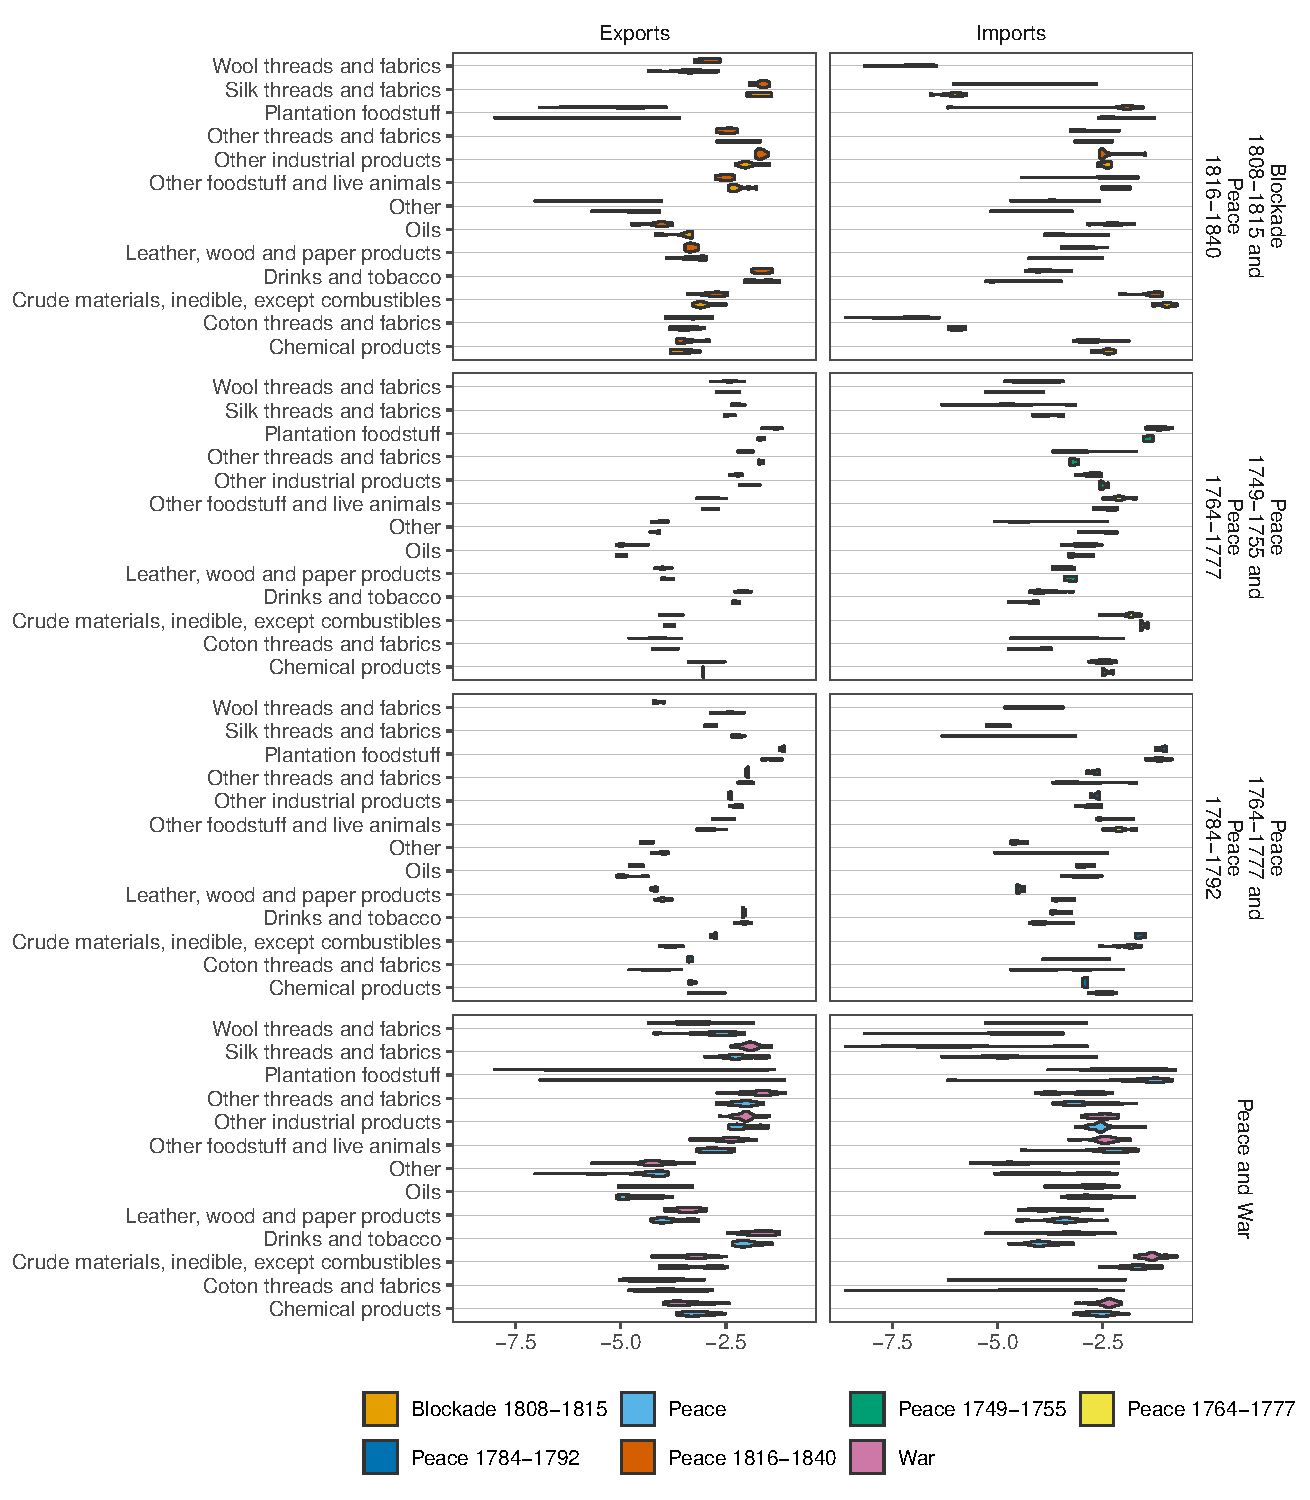
\includegraphics[scale=.9]{violin_nat_sitc1_XI1}
\end{figure}
\begin{figure}[h!]
\caption{Change in composition of trade}
\label{fig:violin_nat_sitc1_XI2}
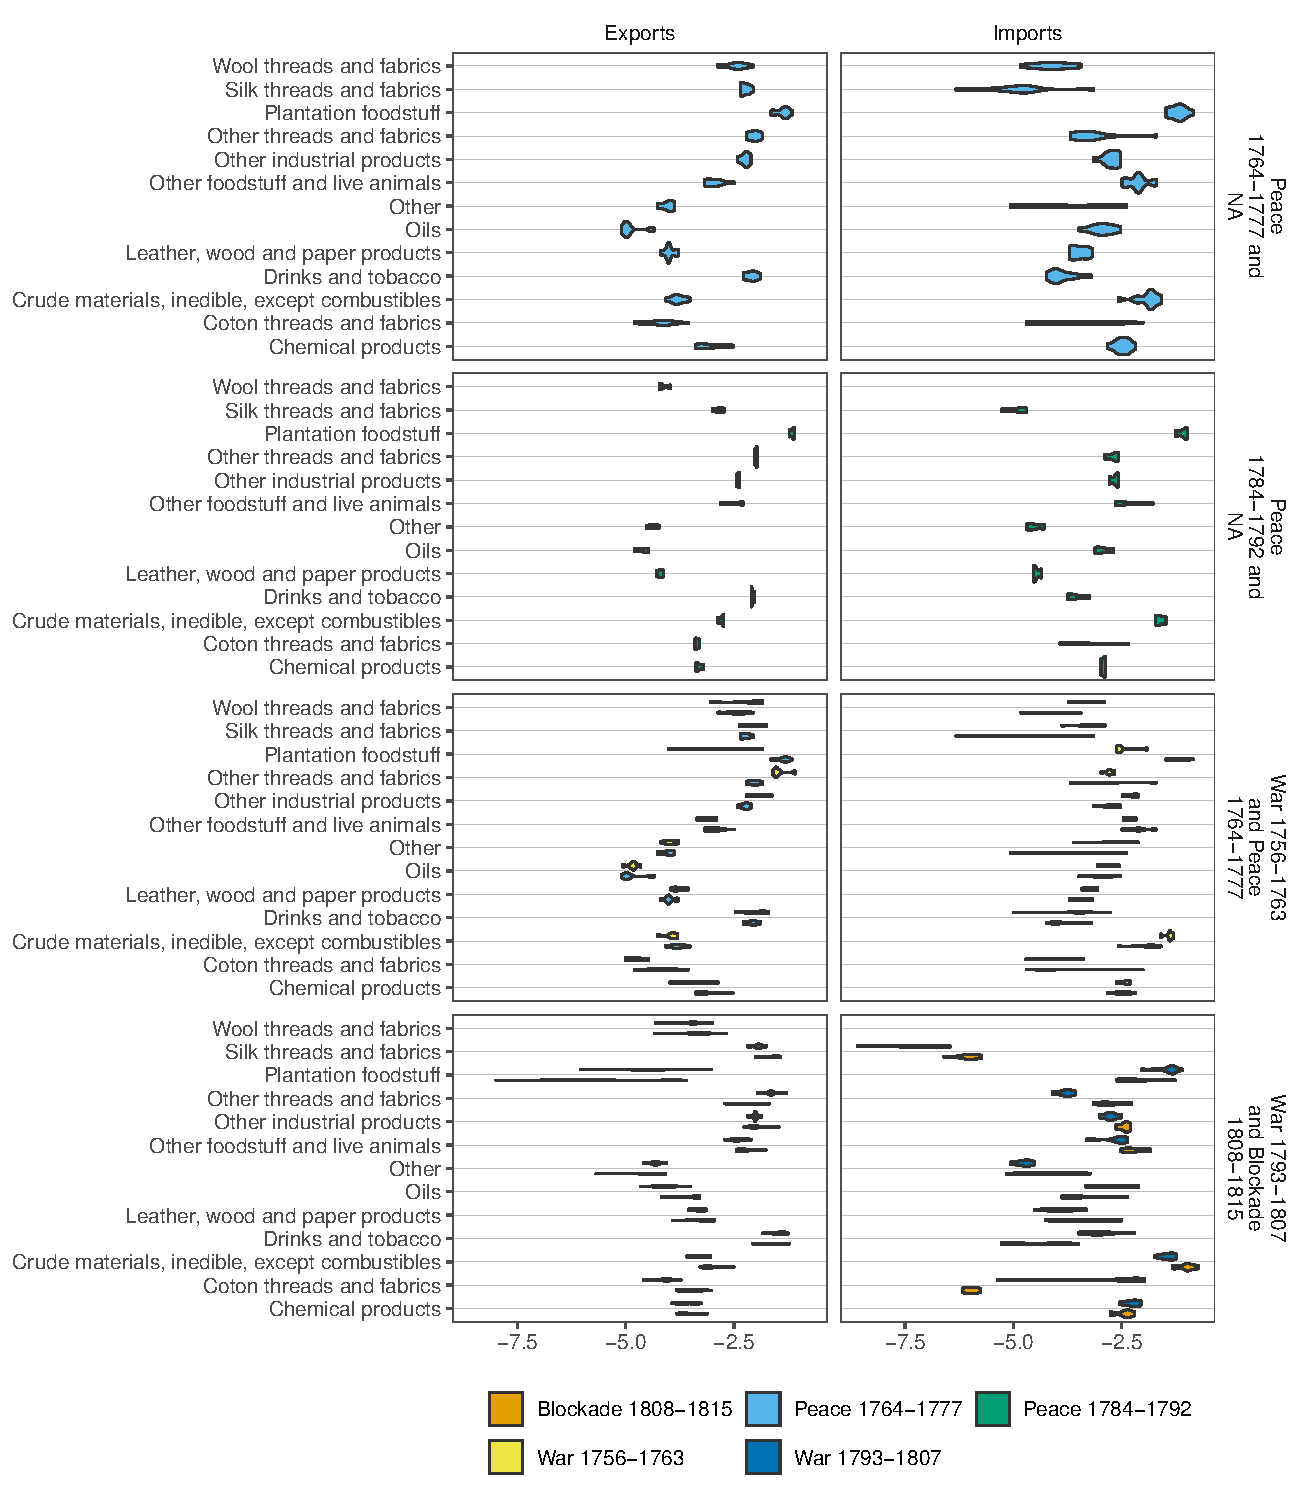
\includegraphics[scale=.9]{violin_nat_sitc1_XI2}
\end{figure}

\begin{figure}[h!]
\caption{Change in composition of trade - Without plantation foodstuff}
\label{fig:violin_nat_sitc0_XI1}
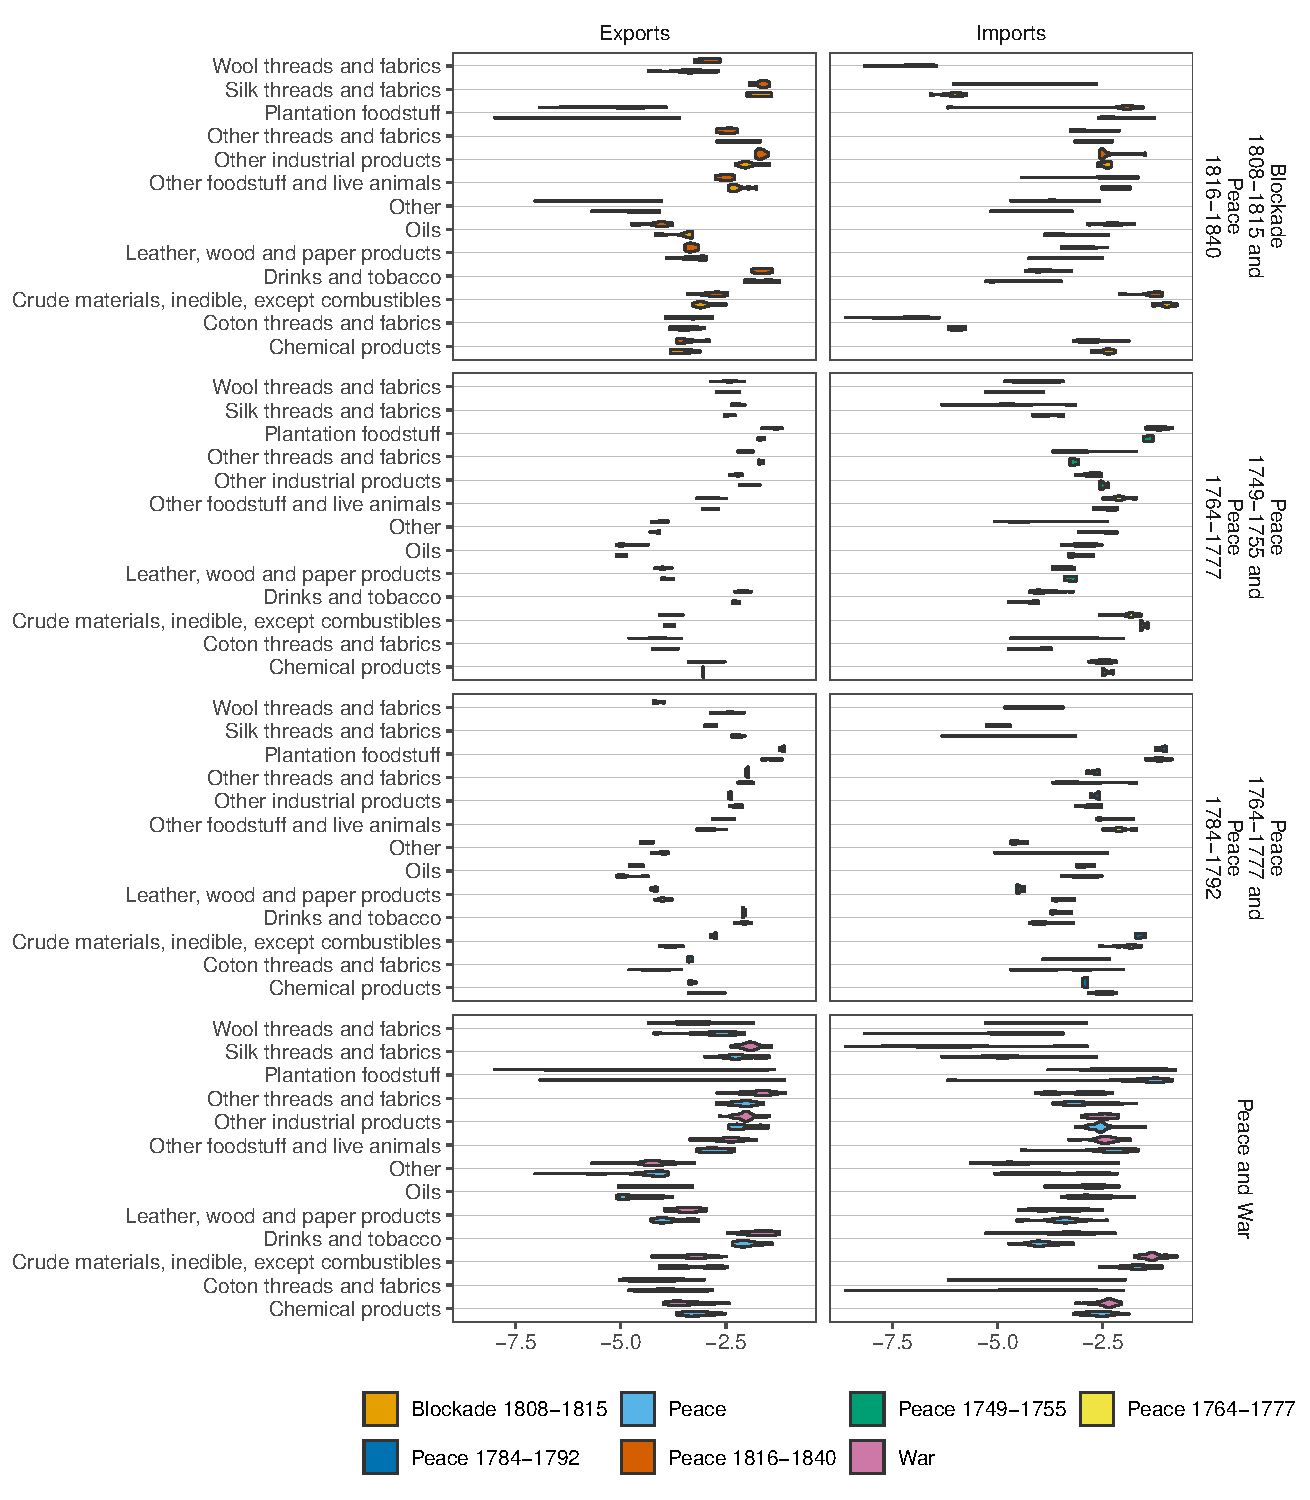
\includegraphics[scale=.9]{violin_nat_sitc0_XI1}
\end{figure}
\begin{figure}[h!]
\caption{Change in composition of trade - Without plantation foodstuff}
\label{fig:violin_nat_sitc0_XI2}
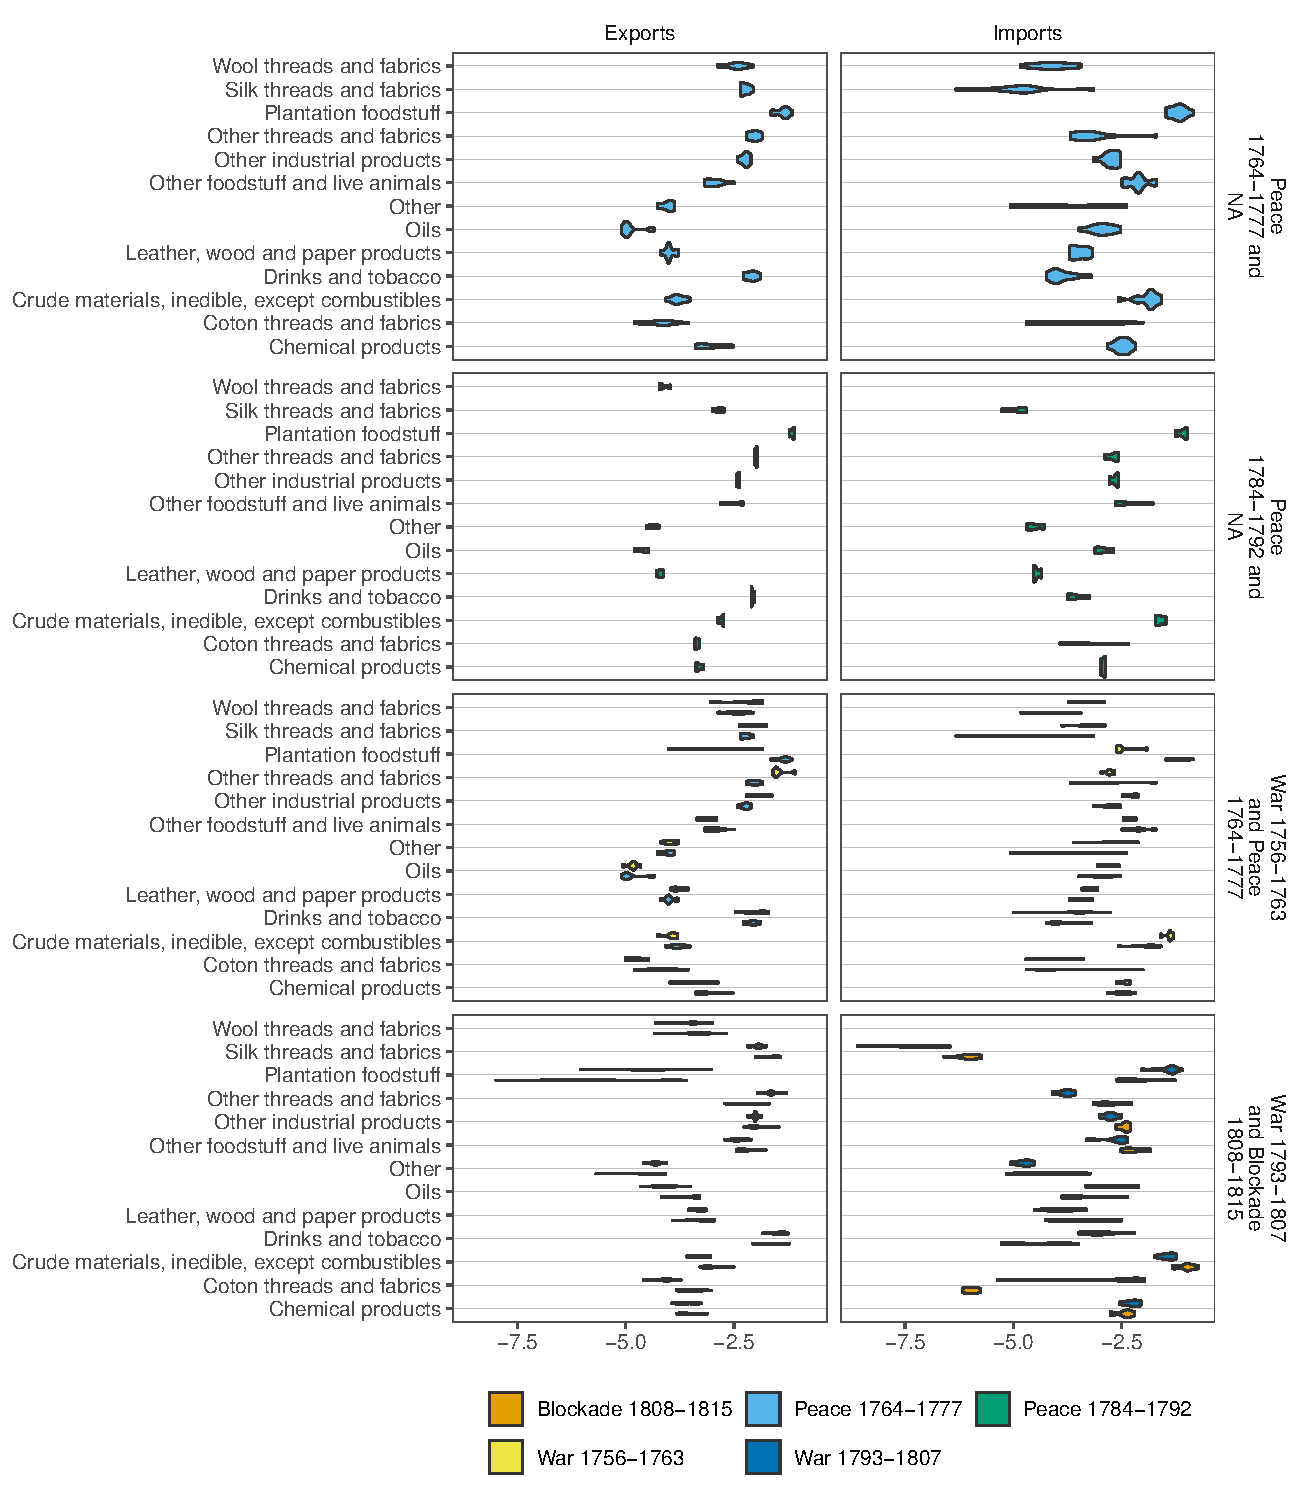
\includegraphics[scale=.9]{violin_nat_sitc0_XI2}
\end{figure}


\begin{figure}[h!]
\caption{Change in geography of trade}
\label{fig:violin_nat_pays1_XI1}
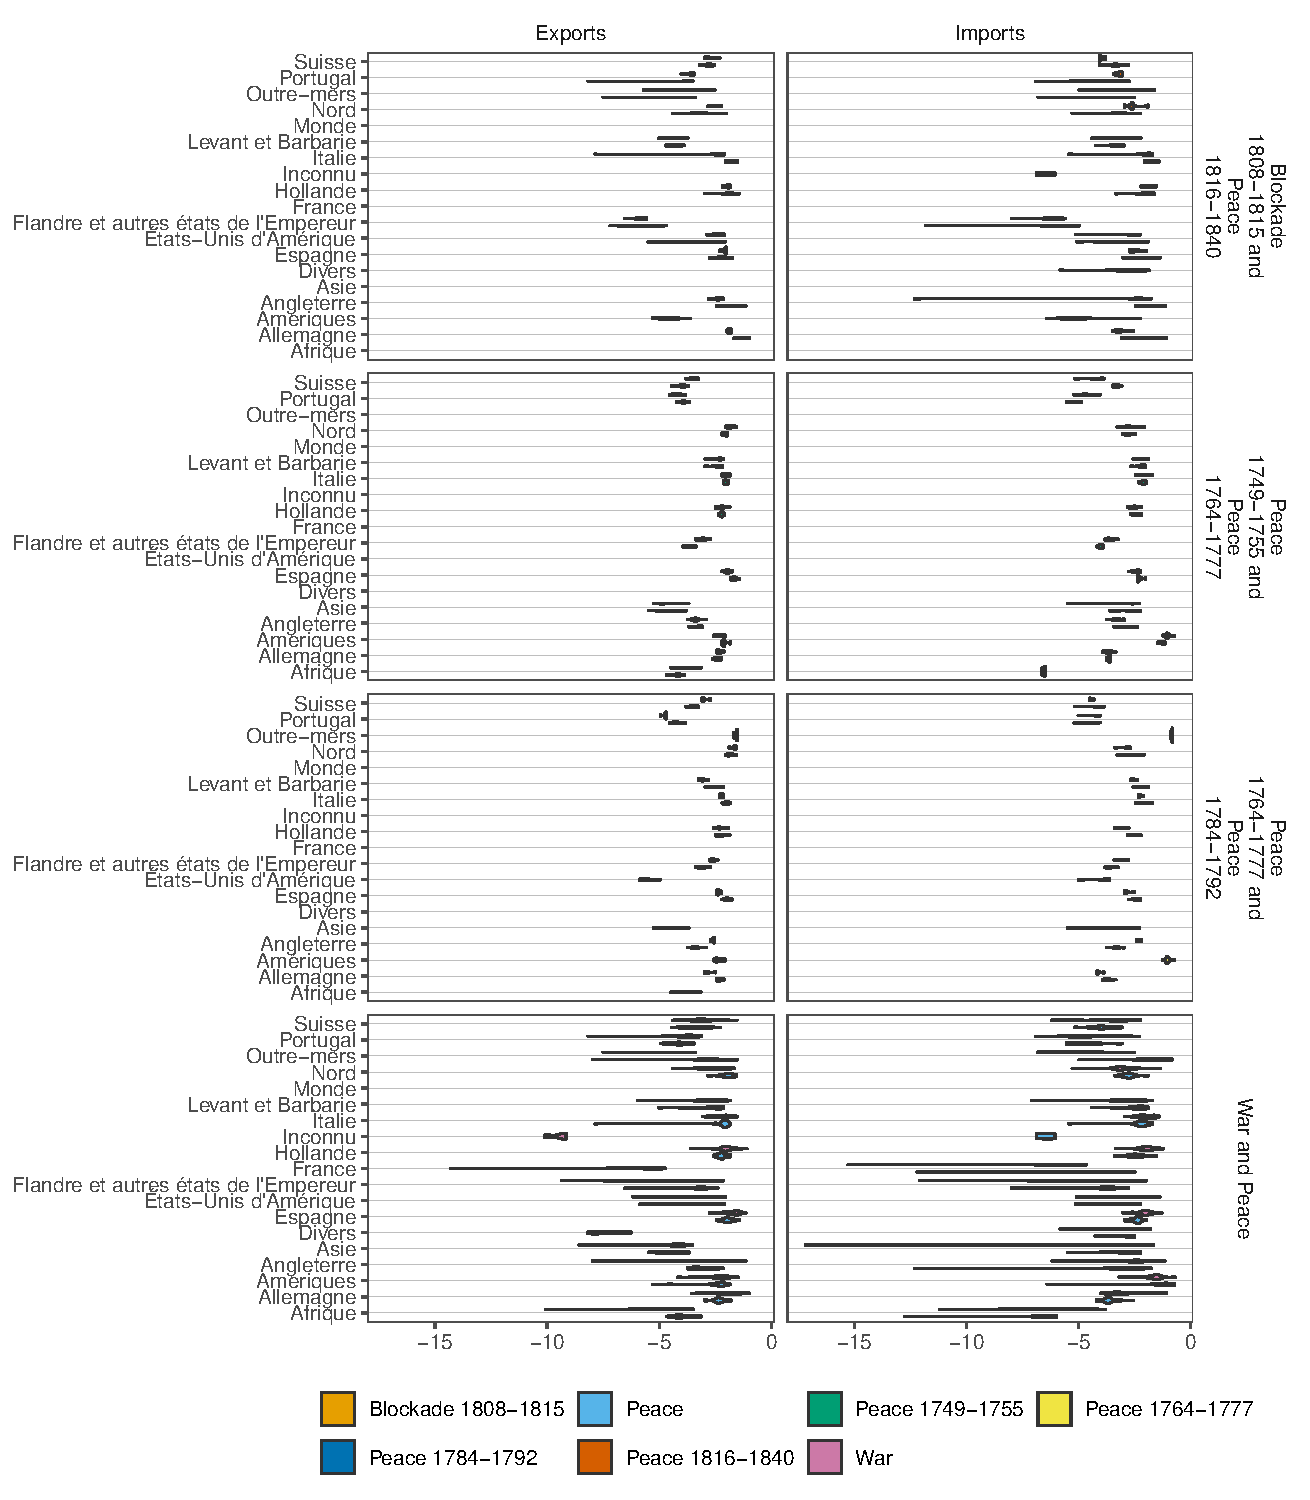
\includegraphics[scale=.9]{violin_nat_pays1_XI1}
\end{figure}
\begin{figure}[h!]
\caption{Change in geography of trade}
\label{fig:violin_nat_pays1_XI2}
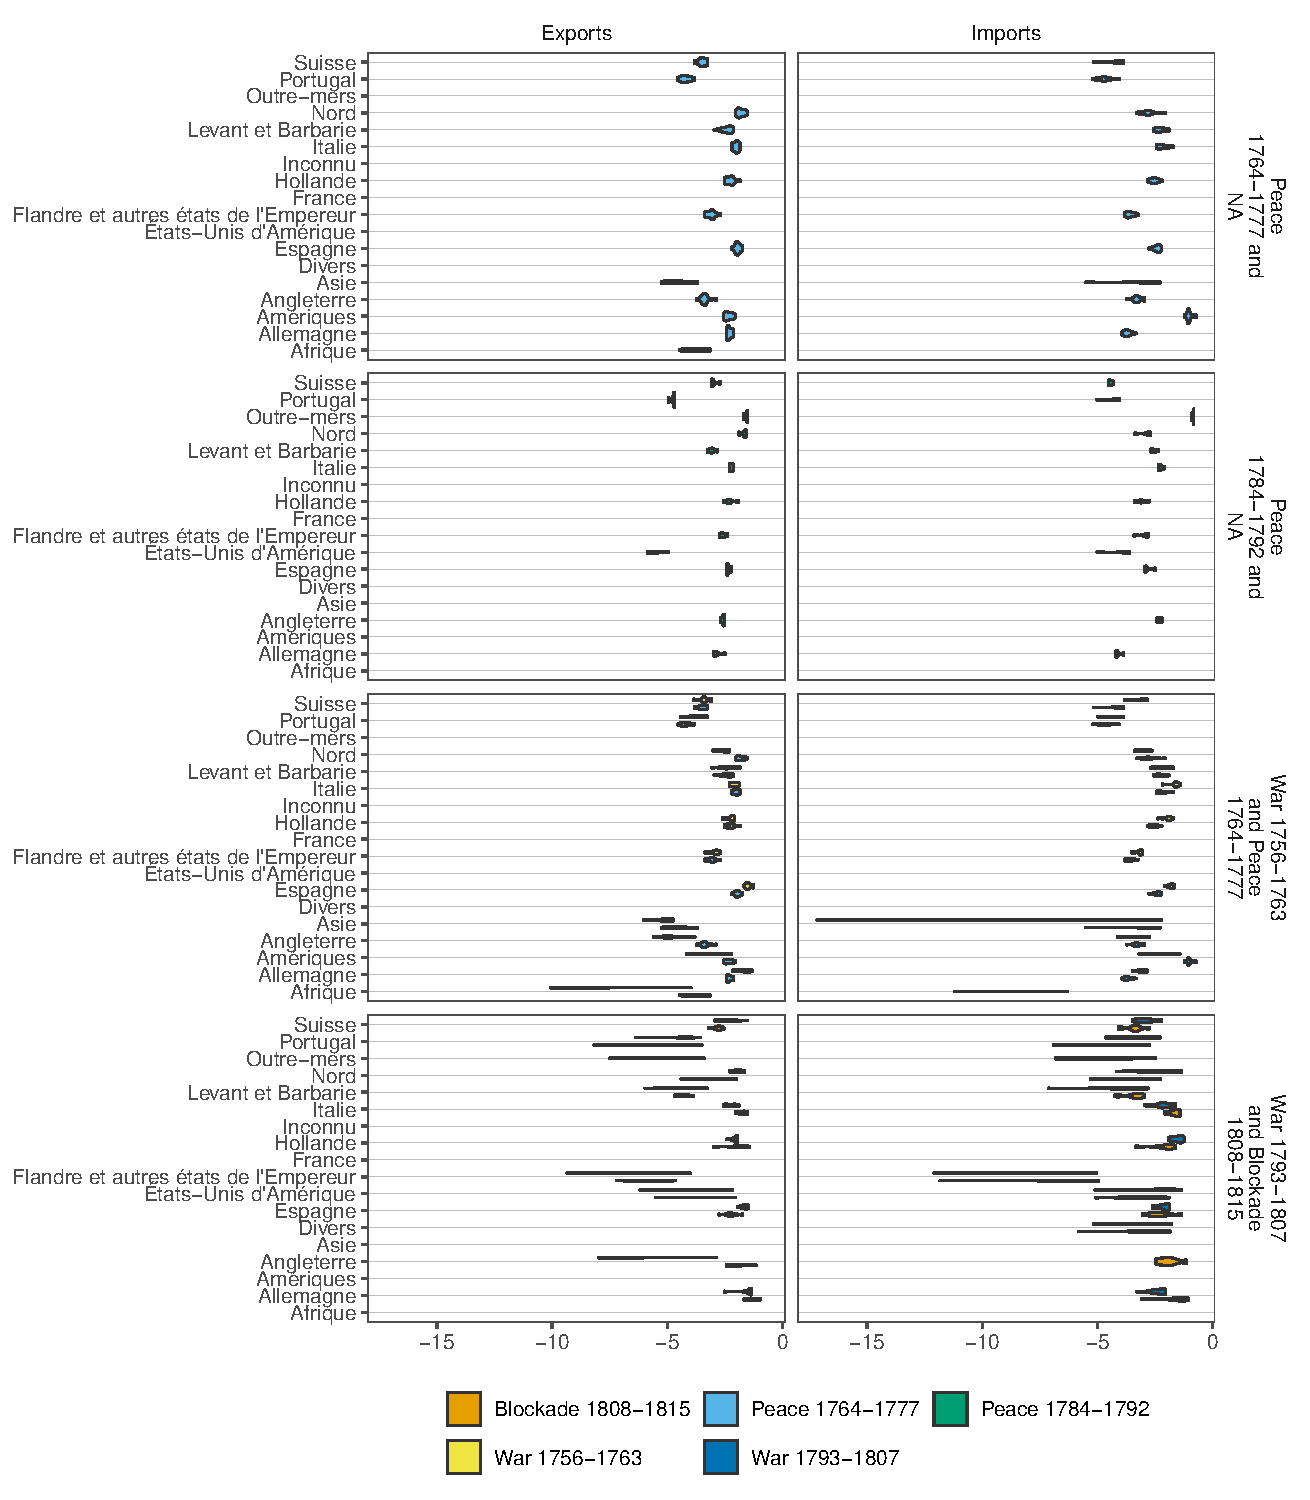
\includegraphics[scale=.9]{violin_nat_pays1_XI2}
\end{figure}

\begin{figure}[h!]
\caption{Change in geography of trade - Without plantation foodstuff}
\label{fig:violin_nat_pays0_XI1}
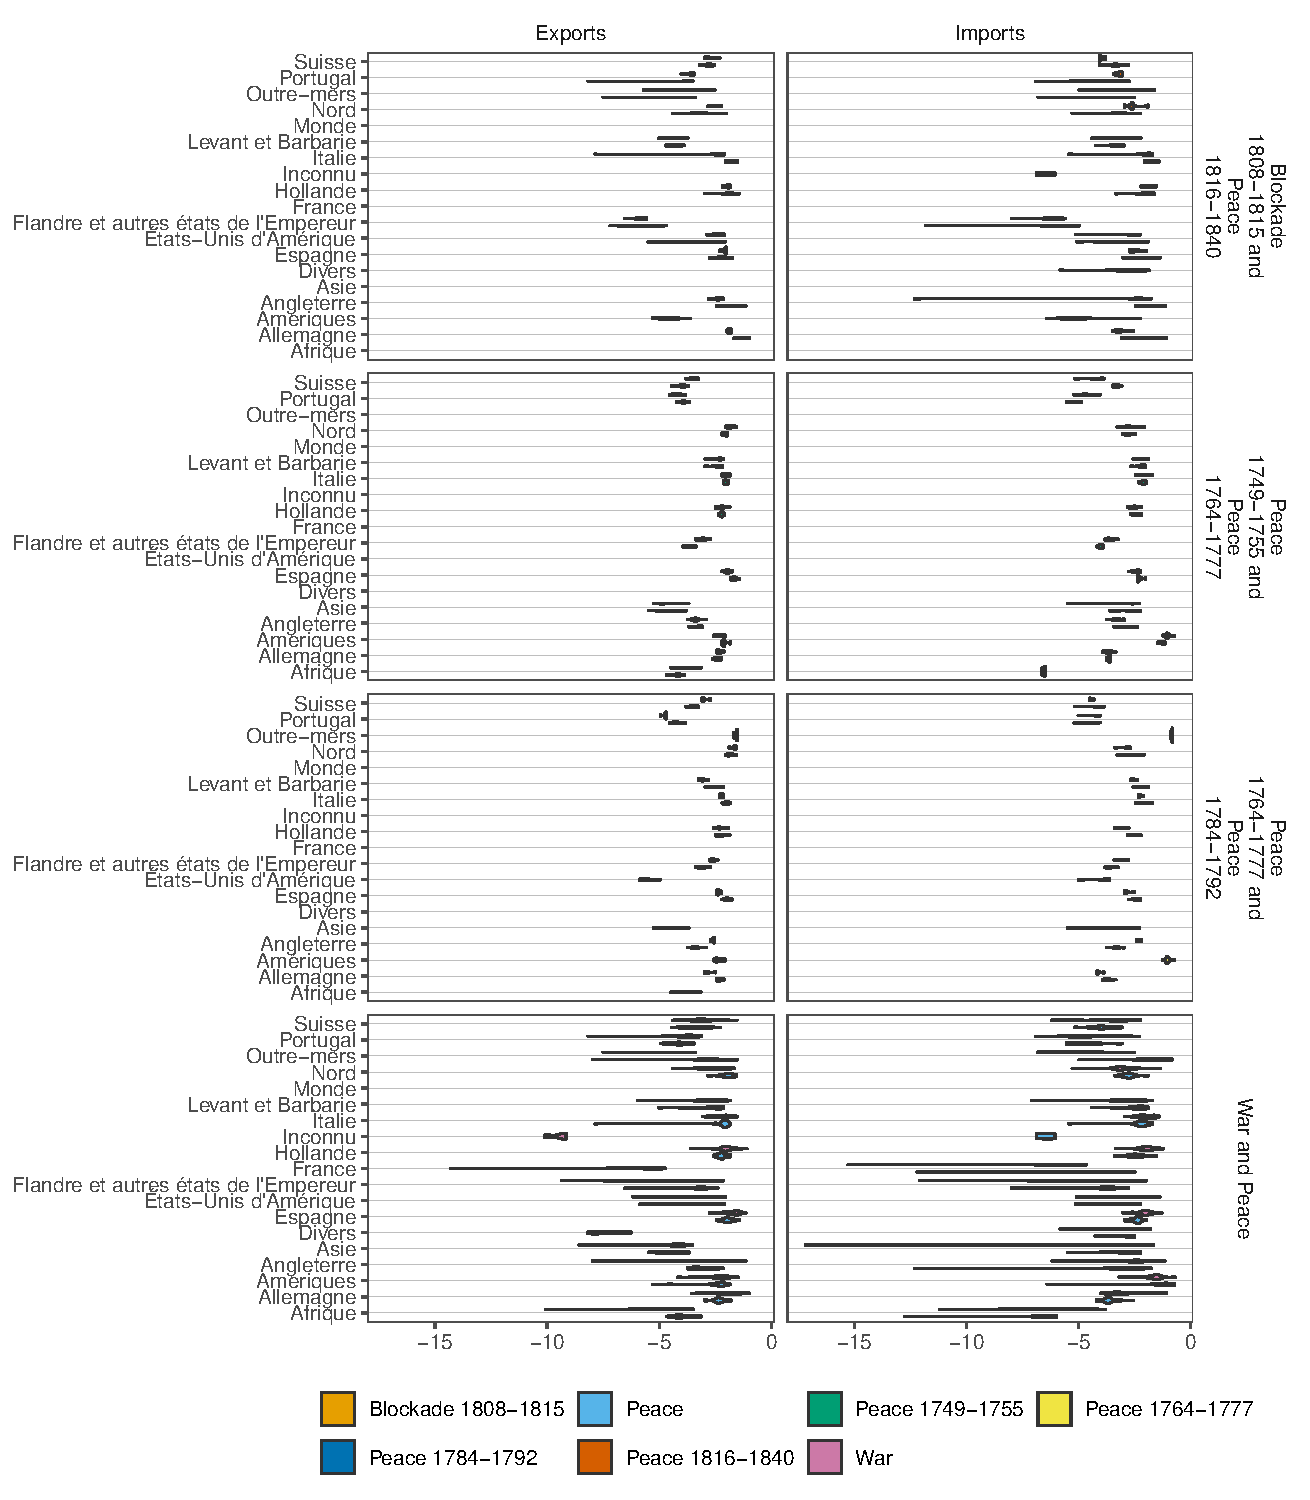
\includegraphics[scale=.9]{violin_nat_pays0_XI1}
\end{figure}
\begin{figure}[h!]
\caption{Change in geography of trade - Without plantation foodstuff}
\label{fig:violin_nat_pays0_XI2}
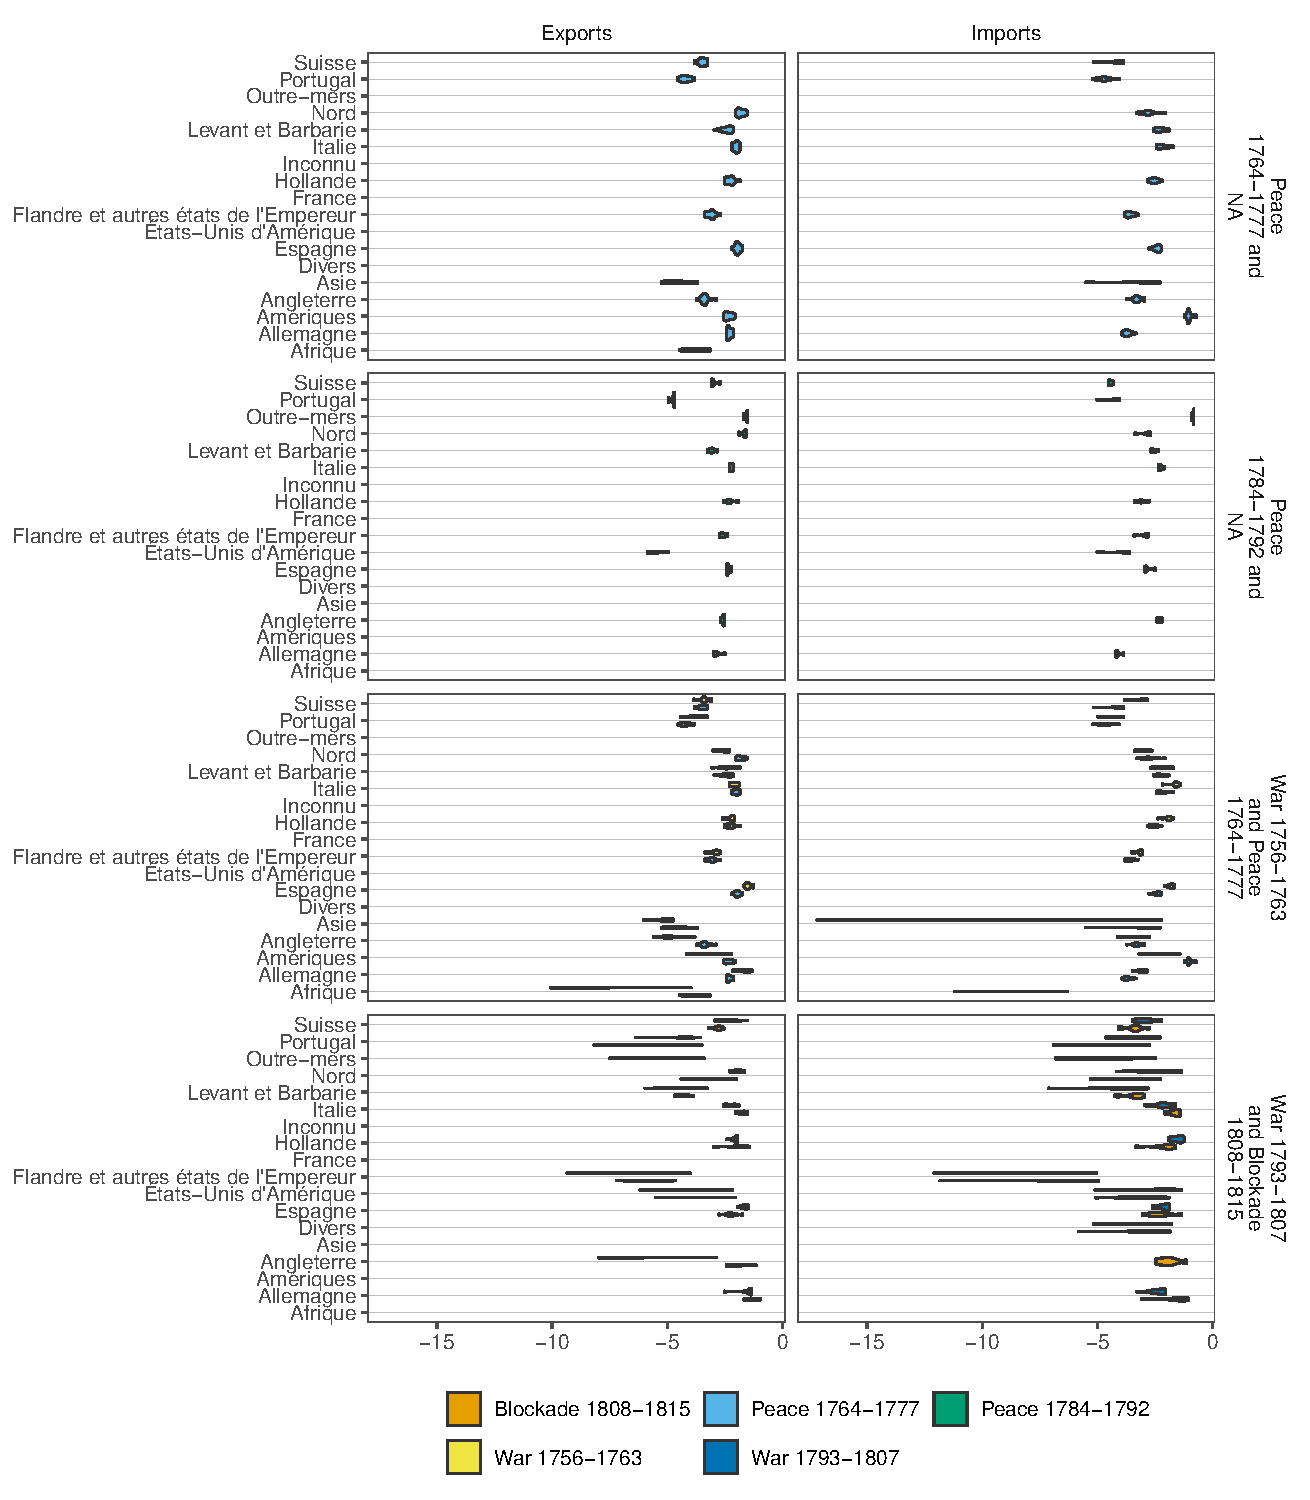
\includegraphics[scale=.9]{violin_nat_pays0_XI2}
\end{figure}

\newgeometry{left=.6in,right=.6in,top=.8in,bottom=.8in,}

\section{Data and sources} \label{sec:dataset}
We use data from the TOFLIT18 project (see \href{http://toflit18.medialab.sciences-po.fr/\#/home}{here}). They come from the archives of the French \textit{Bureau de la Balance du Commerce} and, subsequentely, the \textit{Bureau des archives du commerce}.
This institution was created in 1713, after the Treaty of Utrecht, which followed the Spanish Succession War.
While discussing a trade treaty with the British, the French negotiators were positively impressed by the detailed knowledge shown on trade flows by their counterparts, and they convinced the government of the necessity of creating an institution that would keep track of exports and imports from and to France \citep{Charles2011}\footnote{\cite{Charles2011}, in their paper, provide the complete history of the \textit{Bureau}.}.
Starting with the year 1716, local \textit{bureaux des fermes} sent their trade records to the \textit{Bureau} in Paris.
The \textit{Bureau} would then compute aggregate yearly figures for each \textit{direction} (port) and then send them back to the local Chamber of Commerce, so that they could add the values up to 1780.
A mix of local and central source survive from this process. Unfortunately the ``local sources'' mostly did not survive; what we have left are parts of the centralised records.
From 1781 to 1791, the work methods of the \textit{Bureau} changed and a number of years of trade have left little record (1783-1786, 1790-1791).
In 1792, through a decree of the National Assembly, the \textit{Bureau de la Balance du commerce} was abolished and replaced by the \textit{Bureau des archives du commerce}. We have some data on 1792 trade, but trade collection properly started again in 1797, so that we are missing information on 1793-1796.

The data which survived come from different sources.
The two most exhaustive ones are the \textit{Objet Général} and the \textit{Résumé}, which contain trade by product and by partner. 
The former is available for the years between 1754 and 1780 and between 1782 and 1788. There are some missing years, especially in the the period between 1761 and 1767, however starting from 1771 it also contains information on quantities and/or unit prices.
The latter is available between 1787 and 1789 and between 1797 and 1821. It does not include quantities, only values, and the classification of goods it uses is less precise than the one from the \textit{Objet Général}.
Lesser complete sources are Local sources and the \textit{Tableau Général}. Local data are available from 1716 to 1780 and in 1789, which allows for partial reconstruction of total trade.
The \textit{Tableau Général} exists in the French archives that provides French bilateral trade, though not broken down by product (\cite{Romano1957}). 

All sources provide the value of trade in the current French currency. This is the \textit{livre tournois} up to 1795 and the \textit{franc} afterward. The value of the \textit{livre} was fluctuating in the early eighteenth century. In 1726, its value was fixed at a value of 4.505 grams of fine silver \citep{Dewailly1857}. Because of the monetary crisis during the revolution, we use data extracted from published appreciation tables to fix the value of the \textit{livre} at 2.9 grams of silver in 1792 (\cite{Hoffman2000}). The French \textit{franc} contained 4.5 grams of fine silver. We convert the trade flows in fine silver; obviously, this does not solve the inflation issue, but we argue that inflation in terms of silver was relatively limited during that period. \todo[inline, color = RoyalBlue]{Citation here? -- GD Yes, we need to have a deep long conversation about inflation (including how it changes the loss function. Still mulling this one.).}

\subsection{Blockade}\label{app:appendix_blockade}
There were essentially two possible types of blockades \citep{Corbett2004}; the open and the closed blockade. The former consisted of keeping the ships at port, but ready to sail, as soon as the enemy fleet left its harbour. This technique was much less straining for men and ships, but less efficient when it came to blockading. On the other hand, the closed blockade consisted of keeping the rival fleet blocked in its own port, impeding it from exiting. This was much more of an efficient technique, however, the maintenance of both ships and men at sea for such a long time was a substantial issue.
By the end of eighteenth century, the British had implemented a very efficient system of resupply, in which supply ships delivered victuals to the fleet at sea, thus allowing it not to return at port regularly for supplies. 
Also, they were being very careful to provide a balanced diet against scurvy, which passed from being a major issue for sails-men, to accounting for only 2 per cent of British naval patients between 1795 and 1800 \citep{Rodger2005}. On top of this, British had started to coat their ships with copper, to fight the issue of barnacles, oysters and the shipworm, which were seriously hindering the speed and the security of their vessels. This dramatically reduced the possibility of avoid the blockade and allowed British to impede unwanted trade more efficiently.
One would think that the number of ships captured declined as not many ships tried to run the blockade, but that is not confirmed by data on prizes \cite{Benjamin2009}.

\subsection{Historical summary and classification of country grouping} \label{app:historical_summary}
In this section we provide a brief overview of the main wars that took place in Europe in the period of analysis and we explain how we classify the belligerent status (compared to France) of the country grouping at stake. As a general rule, we consider \textit{Outre-mers} as ally and \textit{Levant} as neutral. \\
In 1733, the king of Poland August \textsc{ii}, died heirless and his succession soon became a conflict at European level.
France, Prussia and Spain were trying to limit the desire of expansion of the Habsburg monarchy in Poland. Britain stayed neutral and the war saw an end in 1738, with the recognition of August \textsc{iii} as king of Poland, as the Habsburgs had wished.
In the country classification we used, the ally countries were \textit{Espagne}  and the foe was \textit{Empereur} and and \textit{Allemagne} (as Lorraine and West Germany were at that point mostly controlled by the Habsburg).
It was a land conflict, as opposed to the naval conflicts that followed. \\
No longer than two years later, a very similar event occurred as a consequence of the death of Charles \textsc{iv}.
The Habsburg emperor had not died heirless, however his only heir was a woman; Maria Theresa of Austria.
France, Prussia and the Electorate of Bavaria used the pretext that she was ineligible to succeed to her father, to challenge, once again, the Habsburg power.
Maria Theresa was supported by the Kingdom of Great Britain and the Dutch Republic as well as the Kingdom of Sardinia and the Electorate of Saxony.
This conflict, which was born as a succession issue, soon extended to the New World and became a competition between the French and the British for the control of American colonies.
It ended in 1748 with the Treaty of Aix la Chapelle, where France gave back most the territories it had conquered during the war.
Ally country in this case was \textit{Espagne} and foes were \textit{Angleterre} and \textit{Empereur}. \\
Roughly until the end of the Austrian Succession war, a sort of geopolitical and economic equilibrium between France and British colonies on the North American mainland had prevailed. That was broken as a consequence of an uneven population growth \citep{Findlay2009}.
This set the stage to the following war; the Seven Years War, or French and Indian War, which, as the name suggests, was a world-wide conflict.
As opposed to the previous wars, this was a decisive triumph of Britain over France, which was forced to give up Canada, Cape Breton Island and Grenada, recognized the Mississippi River as the Eastern boundary of its possessions in North American, then ceded those possession to Spain.
France also lost enough influence in its colonies to lead to the end of French colonial ambition in India and, subsequently, to the dissolution of the first Compagnies des Indes \citep{Riley1986}.
French allies in this war were \textit{Allemagne}\footnote{As mentioned in section \ref{dataset}, \textit{Allemagne} was mainly Alsace, Lorraine and Western Germany, which were allied to France.
Our assumption is that "Prussia" is sea trade through the Baltic, i.e. a minor portion of \textit{North}, which, however we code as neutral, since it was dominated by Hamburg - despite the fact that Russia and Sweden were allied to France for most of the war.}, \textit{Empereur}, and \textit{Espagne} for 1762.
Foes were \textit{Angleterre}, and \textit{Portugal}. \\
At the end of the Seven Years War, with the victory of Britain and the subsequent departure of the French, the American colonies, no longer feeling the threat of the French presence on the continent, soon started demanding independence from Great Britain\footnote{The French chief minister, the duc the Choiseul, made a prediction to the effect that with no French presence on the continent to threaten them any longer, the American colonies would soon demand independence from Great Britain \citep{Findlay2009}.
This prediction, as it turned out, was prescient.}.
In 1775 they rebelled against British control over their trade and in 1776 they declared independence.
France, still feeling the humiliation subsequent to the Seven Year War, in 1778 entered the fray on the colonies' side, soon followed by Spain.
Spanish and French \footnote{France had been investing in its Navy following the preceding defeat \citep{Findlay2009}.} fleet together outnumbered the British Navy and were able to force Britain to surrender and end the war with the Treaty of Versaille in 1783.
In this setting, ally were there \textit{Espagne}, \textit{Etats-Unis}, and \textit{Hollande} from 1780; foe was only \textit{Angleterre}. \\
At the end of the war, despite the victory obtained, French finances were suffering to the extent that Calonne, the finance minister at the time, was forced to the summoning of the Estates-Generales in 1789, which then led to the start of the French Revolution.
This event was followed by a larger conflagration with respect to previous mercanilist wars, into which an ideological dimension had been injected \citep{ORourke2006}.
In 1792 France declared war on Austria and Prussia, and the following year to Great Britain.
The subsequent conflict lasted for nearly thirty years, with only two brief interruption between 1802 and 1803 (Peace of Amiens) and between 1814 and 1815.
Almost immediately, France banned the import of all British goods; Britain responded by blockading French coasts and impeding French ships to exit the port.
From the very beginning, this created a big problem for neutral countries, which wished to continue trade with both belligerent actors.
As a consequence, a second League of Armed Neutrality was created, in which Russia, Prussia, Denmark and Sweden took part.
This alliance was not long-lasting, as Britain responded with a ban on trade with the league, and bombed Copenhagen, thus ending this agreement.
This conflict ultimately ended with Napoleon's disastrous invasion of Russia in 1812, which was followed by the invasion of France in 1814 and a subsequent peace treaty signed in Ghent.
The two main players of this conflict were, of course, Britain and France.
However, because of the victories and defeats of one and the other, sides of other countries changed continuously and it was harder to code in our country classification. Table \ref{war_peace} reports our choices of the position of all countries in all wars throughout the century. 
\textit{Allemagne} was mainly aligned with Austria till 1800: so it was a foe between 1792 and 1800, neutral between Campo Formio became an ally in 1805 (till 1813), and then became again a foe after the battle of Leipzig to France.
\textit{Angleterre} was an enemy all throughout.
\textit{Espagne} fought France for the period 1793 and 1794, she became then an ally until 1807 (with the exception of 1795, in which she was neutral), and then again an enemy from 1808 onwards.
\textit{Empereur} is Austria, whose position was easy to adjudicate. It was a foe until Campo Formio (June 1801), neutral till the Third Coalition (1805), then a foe in 1805, to become neutral again in 1806 until 1808.
Lastly, after one more year of neutrality in 1809, she became an ally starting from 1810, and declared war again in 1813.
\textit{États Unis} was always neutral throughout the war, except for the un-declared war between 1798 and 1800 and it co-belligerance against the United Kingdom from 1812 to 1814.
We classify them as "Allies" during this period of co-belligerence.
\textit{Hollande} fought France till 1794 and was then aligned to it till late 1813, when William-Frederik of Orange-Nassau took power.
\textit{Italy} was briefly a foe until 1796, then neutral until 1813, and then again a foe starting 1814.
\textit{Levant} stayed out of the war, except when the French invaded Egypt from 1798 to 1801.
Concerning \textit{Nord}, Sweden and Russia were alternatively neutral, foes or allies. Denmark was an ally. Yet, as the biggest share of trade was represented by Hamburg, whenever the component of \textit{Nord} were not on the same side in a war, we code them all in the position of Hamburg. \textit{Nord} was mainly neutral, except when it was occupied and then annexed by France from 1808 to 1813.\footnote{Obviously, we cannot proceed this way for the computation of naval supremacy, see \textit{infra}.}
\textit{Outre-mers} mainly includes French colonies and we treat it as an ally throughout.
\textit{Portugal} was neutral until 1798 and then became a foe in 1802.
It was again neutral for a short period between 1803 to 1806 and then became a foe starting from 1807.
Finally, \textit{Suisse} was neutral until 1797 and then an ally until 1813, and then neutral again in 1814. \\
Figure \ref{Number_of_protagonists} sums up the data by showing the number of French allies, foes and neutral for each war and year of interest. 

\subsection{Trade partners} \label{trade_partners}
Trade partners are not consistently designed in the original data. 
For example, In the \textit{Tableau Général} (from 1716 to 1782), the number of partners varies between 14 and 23 and between  16 and 26 in the \textit{Résumé} (from 1787 to 1821).
Often, partners are not single countries but rather groups of countries.
Many destinations get broken down into smaller destinations in later periods or even disappear to be replaced by other smaller entities.
To bypass this problem we have created a classification of countries, which is consistent for the whole period (such that we have nearly one observation for each group for each year).
This classification identifies only twelve groups: \textit{Allemagne}, \textit{Angleterre}, \textit{Espagne}, \textit{Flandre et autres États de l'Empereur}, \textit{Hollande}, \textit{Portugal}, \textit{Suisse}, \textit{Levant}, \textit{Italie},  \textit{États-Unis}, \textit{Outre-mers} and \textit{Nord}. Many are self-explanatory, though it should be underlined that trade with \textit{Angleterre}, \textit{Portugal} and \textit{Espagne} includes trade with all their controlled territories. \\
\textit{Outre-mers} regroups all intercontinental French trade (mainly with French colonies) except for North Africa and the Ottoman Empire that are included (along with Greece) in \textit{Levant}.\\
\textit{Nord} designates trade north of the Low Countries.
This region comprises Sweden, Denmark, Hanseatic ports (mainly Hamburg, Bremen, Lubeck and Danzig), Prussia and Russia\footnote{Trade with Denmark is identified separately from 1733, trade with Sweden from 1734 and trade with Russia from 1744.
We always account for them together under \textit{Nord}} \citep{Charles2018}.\\
\textit{Italie} was used as a geographical expression.
The main French trade partners there were the Kingdom of Piedmont and Sardinia and Genoa.
Still, minor flows were also directed to Milan, Naples, Venice, Tuscany, Papal States...\\
\textit{Flandre et autres États de l'Empereur}  (\textit{Empereur} for short) is mainly modern Belgium before the Revolutionary and Napoleonic Wars and mainly Austria after it. At that point, modern Belgium is annexed by \textit{Hollande}. \\
\textit{Allemagne} encompasses mainly Western Germany, including Alsace, Lorraine during the \textit{Ancien Régime}. \\
We have not attempted to take into account the extensive territorial re-arrangements during the Revolutionary and Napoleonic Wars.
The extension of France in the Low Countries, Germany and Italy changed the actual extent of the \textit{Allemagne} and \textit{Italie} partner.

\subsection{MANOVA test}

In order to test this we conduct a Multivariate Analysis of Variance (MANOVA), allowing for heterogeneous co-variances, using the affine-invariant modification by \cite{Krishnamoorthy2004} of the test proposed by \cite{Nel1986}. The two mean vectors here are the 13- or 9-dimensional vectors whose components are the SITC or the country trade shares respectively and the groups are the war-peace periods or the pre-war and post-war peace periods. 
We do it for imports, exports and imports exports together and then excluding plantation foodstuff. Resulting p-values are reported in tables \ref{tab:manova_test_sitc} and \ref{tab:manova_test_pays} and figures \ref{fig:violin_nat_sitc1_XI1} to \ref{fig:violin_nat_pays0_XI2} show the distribution for each sitc and country in each period. \\
Considering a 5\% threshold for rejecting the null hypothesis of equality of means, we observe from table \ref{tab:manova_test_sitc} that there is undoubtedly a change in trade structure by products between war and peace periods overall. The p-value is zero, which implies that at least one sitc category (which is not necessarily Plantation foodstuff, because the p-value increases after removing it from the analysis) changes between the two periods. Narrowing down our analysis we proceed to observe the difference between trade structure in war and preceding or following peace periods. Both because of lack of data and of very short peace periods, the comparison is not always possible. We could only examine the difference between Seven Years Wars and the 1764-1777 peace, 1764-1777 peace and War of American Independence, French Revolutionary Wars and Continental Blockade and Continental Blockade and the 1816-1840 peace. In the first case we observe that we can reject the hypothesis that the two mean vectors are the same, i.e. at the end of the Seven Years War there was a clear shift in composition of trade. The only exception is for the case of aggregate imports and exports, including Plantation Foodstuff, where we fail to reject the null hypothesis, however individually on imports and exports the significance for rejection is quite high. Such dramatic change did not happen with the beginning of the War of American Independence, we observe in fact that the p-values are all above the 5\% level, and even if they decrease upon eliminating Plantation Foodstuff, they remain above the threshold. Hence in this case we can say that the outburst of the conflict did not have consequences on French trading pattern. The same cannot be said for the difference between French Revolutionary Wars and Continental Blockade, when there was once again a clear shift in composition of trade, which does not only depend on Plantation Foodstuff, i.e. the share of at least another category of the SITC classification changed significantly between the two periods. We also observe that the change was longer lasting. At the end of the Continental Blockade in fact, France does not seem to recover its pre-Blockade trade structure. This cannot only be due to the fact that it lost its main source of Plantation Foodstuff import and re-export, because even excluding this category the result is consistent. 

\subsection{French Budget} \label{french_budget}

The French Navy budget is one of the better known of the Ancien Régime budgets. Unfortnately, it is still quite difficult to determine. We try to compute a serie from 1740.
The canonical source is \cite{Legoherel1965}.
An important printed source is \cite{Neuville1898}. \cite{Dull1975, Villiers2002} have useful insights.
There is a long-term serie (1691-1782) probably coming from \textit{La Cour des Comptes} in the Bibliothèque Nationale (\textit{Nouvelles Acquisitons Françaises}, 5399).
It is notoriously an under-estimation (\cite{Villiers2002}).
We exclude the source from 1740 to 1760 that is found in the \textit{Archives Nationales} (G7 1830) because, according to \cite{Villiers2002}, it includes the colonial budget.
For 1745 and 1748-1770, Neuville and Villiers provide numbers from the intendant du Trousset d’Héricourt that are plausible.
We use them.
They are is 2.5 \% higher than the BN source.
So for 1740-1744, 1746 and 1747 we use the BN numbers multiplied by 1.025
For 1776-1783, \cite{Dull1975}[p.348-350] has worked out that the "best" source comes from Castrie.
We use them.
They are 6\% higher than the BN source.
So for 1771-1775, we use the BN source multiplied by 1.06.

For 1783-1788, we use Pierre-Victor Malouët as reported by \cite{Villiers2002}. For 1789-1791, we use rough estimates by Charles-François Lebrun as reported in \cite[][ p. 259 and 332]{Marion1914}. For 1801, we use \cite{Branda2007},. We distribute the "imperial arrears" (i.e. the money still owned by the State at the fall of Napoleon that had not been affected to a budget year) over the years 1812-1814 on a pro-rata temporis basis.
Finally, for 1816-1825, we use the official publications named ``Compte Rendu... ...'' \citep{1814,1818,1826})\todo[inline, color = YellowGreen]{Better ? These are coming from the BNF}
We try to determine what has been actually expended each year rather than each year’s budget, as before the reform of 1822 these were not the same thing (see \cite{Kott2019}).
Finally, for 1793-1800, the lack of sources due the total disorganisation of French finances at the time leads us to simply assume a constant growth rate of the budget between the (quite uncertain) 1792 budget and the (much more reliable) 1801 budget.

The resulting series is used in the paper.




%plainnat


\end{appendix}

\tableofcontents

\listoftodos[Notes]

\end{document}

